\documentclass[11pt]{book}

\usepackage{fullpage}
\usepackage{graphicx}
\usepackage{cite}
\usepackage{times}
\usepackage{url}
%%\usepackage{hyperref}
\usepackage{setspace}
\usepackage{fancyhdr}
\usepackage{ifthen}
\usepackage{listings}
\usepackage{color}
\usepackage[section]{placeins}
\usepackage{xtab}
\usepackage{url}
\usepackage[vlined]{algorithm2e}
\usepackage{float}
\usepackage{multirow}
\usepackage{paralist}
\usepackage[htt]{hyphenat}

\setcounter{topnumber}{2}
\setcounter{bottomnumber}{3}
\setcounter{totalnumber}{4}
\renewcommand{\topfraction}{0.5}
\renewcommand{\bottomfraction}{0.95}
\renewcommand{\textfraction}{0.1}
\renewcommand{\floatpagefraction}{0.7}

\setlength{\abovecaptionskip}{3pt}
\setlength{\belowcaptionskip}{3pt}

\pagestyle{fancy}
\setboolean{@twoside}{false}
\setlength{\headsep}{25pt}
\setlength{\headheight}{14pt}

\definecolor{dkgreen}{rgb}{0,0.6,0}
\definecolor{gray}{rgb}{0.5,0.5,0.5}
\definecolor{mauve}{rgb}{0.58,0,0.82}

\lstset{frame=tb,
  language=C++,
  columns=flexible,
  basicstyle={\linespread{0.9}\small\ttfamily},
  breaklines=true,
  captionpos=b,
  aboveskip=0.2in,
  belowskip=0.2in,
  numberstyle=\tiny\color{gray},
  keywordstyle=\color{blue},
  commentstyle=\color{dkgreen},
  stringstyle=\color{mauve},
  tabsize=4
}

\begin{document}

\thispagestyle{empty}

\doublespacing

\vspace*{0.5in}

\begin{center}
\LARGE{\textbf{Time Warp Simulation on Multi-core Processors and Clusters}}

\vspace*{0.4in}

  {\large A thesis submitted to the\\[0.20in]
    Division of Research and Advanced Studies\\
    of the University of Cincinnati\\[0.20in]
    in partial fulfillment of the\\
    requirements for the degree of\\[0.20in]
    \textbf{MASTER OF SCIENCE}\\[0.20in]
    in the School of Electric and Computing Systems\\
    of the College of Engineering and Applied Sciences\\[0.20in]
    August xx, 2015\\[0.20in]
    by\\[0.20in]
    \textbf{Doug Weber}\\
    BSEE, University of Cincinnati, 2014\\}
  \vspace{0.5in}
  {\large Thesis Advisor and Committee Chair:  Dr. Philip A. Wilsey}
\end{center}

\clearpage

\setcounter{page}{1}
\pagenumbering{roman}
\clearpage

\chapter*{Abstract}

Parallel Discrete Event Simulation (PDES) systems have traditionally been designed for either
clusters using message passing communication \emph{or} for shared-memory multiprocessors using
shared data structures but not both.  The fine granularity of PDES applications makes the
communication latency of message passing a target issue.  Message passing, however, is necessary to
scale up the computational power and memory required for larger simulation models that would be
limited in a single shared-memory processor.  Shared memory communication, on the other hand, means
that the latency of exchanging events is significantly reduced since buffer copying and network
communication can be avoided.  The computational power of clusters composed of multi-core processors
requires the combination of both forms of communicating processes in ways that effectively exploits
the computational power of parallelism that balances the high disparate message latencies found
within and between the processing cores.  \emph{The challenge of PDES in this environment is that
  discrete-event simulation models are primarily fine-grained and generally highly sensitive to
  message latency costs.}

This thesis explores the design of a Time Warp synchronized PDES simulation kernel called
\textsc{warped2} that is designed and evaluated for efficient execution on multi-core processors and
clusters of multi-core clusters.  The \textsc{warped2} simulation kernel uses a hybrid approach
where a set of mulithreaded processes communicate with message passing between nodes but threads
within each process communicate through shared data structures within a node.  To attack the
imbalanced latencies in these two communication mediums, the \textsc{warped2} simulation kernel
supports a variety of partitioning methods to minimize communication between nodes and also to
assist memory referencing patterns within the cores of a compute node.  If the logical processes
(LPs) of the simulation model are partitioned properly, then the interprocess communication will be
minimized and the simulation models can scale to large clusters of multi-core processors.

A hybrid communication approach, however, adds some significant complications that make it difficult
to optimize the simulation mechanism for the best performance.  The first problem that must be dealt
with, which is common to any multithreaded application, is the high cost of thread synchronization
to protected shared data structures.  This problem not only adds significant overheads in the
simulation mechanism (dispatching of local events and processing events) but with the standard
runtime and message passing libraries as well.  A few of the solutions what will described include
separating data structures for thread local use to eliminate synchronization, using spinlocks to
reduce lock acquisition latency, using alternative multithreaded memory allocators, and using a
separate thread to handle message passing communication.

The second, and more Time Warp specific problem, arises with a hybrid communication model is with
developing asynchronous global virtual time (GVT) and termination detection algorithms that are
usually designed for either shared-memory multiprocessors \emph{or} message passing systems, but not
both.  For both GVT and termination detection, a two level approach for each will be discussed and
analyzed.

Experimental analysis will be performed on SMP nodes and clusters to gain a better understanding of
the tunable performance, communication, and memory parameters of \textsc{warped2}.  Preliminary
results indicate that any optimization that minimizes thread synchronization is usually preferable
on a single SMP node even if rollbacks increase and event processing efficiency decreases.  On a
cluster, minimizing remote communication is the key to minimizing rollbacks and increasing
performance.  Funneling communication to a dedicated thread has been shown to be more effective than
a multi-threaded communication model which means that a high synchronization costs in the message
passing library is more limiting than an increased communication latency.

%% DOUG: should you also comment on your findings regarding fossil collection in this
%% abstract?  i will probably have stronger direction on this after i finish the thesis.

%% DOUG: should you have a final paragraph that comments on the feasibility/scalability of
%% PDES performance results on these multi-core processors and clusters?

\chapter*{Acknowledgments}

First and foremost, I would like to thank Dr.\ Wilsey for his guidance throughout my research
experience. It has been a great experience working with him and I have learned more than I ever
thought I would.

I would also like to thank Sounak Gupta for his work with the pending event set in \textsc{warped2}
and AJ Alt for his work with the initial development of the \textsc{warped2} API and sequential
kernel.  My research would not have been possible without them.  Also, thanks to all previous
students in the Experimental Computing Lab who contributed to the development of the original
\textsc{warped} simulation kernel.

Thank you to my family for being supportive throughout my entire education at the
University of Cincinnati.

\tableofcontents    \markright{ }
\listoffigures      \markright{ }
\listoftables       \markright{ }
\listofalgorithms   \markright{ }
\lstlistoflistings  \markright{ }

\clearpage
\pagenumbering{arabic} \setcounter{page}{1}

\chapter{Introduction}\label{intro}

%% Background
Many physical systems can be represented by a discrete-event simulation model where events represent
state changes that occur in discrete time intervals.  Examples of such systems are: communication
networks, digital logic circuits, transportation systems, or disease outbreaks \cite{law-00}.  In
order to gain a better understanding of these systems, researchers develop models of the systems and
perform simulations on computing platforms.  These \emph{Discrete Event Simulation} (DES) models can
take a long time to simulate large, complex systems by sequentially processing events.  These long
simulation times have led researchers to design parallel algorithms to run simulations on parallel
computing platforms.  The field of study that deals with parallel algorithms to speed up discrete
event simulations is known as Parallel Discrete Event Simulation (PDES)
\cite{fujimoto-90,fujimoto-00}.

Parallel algorithms can be written to target many different architectures that support parallelism
such as shared-memory multiprocessors, clusters, or any other type of system that support parallel
execution \cite{culler-97,patterson-11}.  Furthermore, communication between concurrent workers in
the system can be achieved by using shared data structures or by passing explicit messages between
threads.

The Time Warp Mechanism \cite{jefferson-85,fujimoto-90}, which is the focus of this thesis, is one
approach to synchronize PDES where causal dependencies of events are not enforced before processing
an event.  A method of undoing erroneous computation and canceling incorrectly sent events must be
implemented in a Time Warp system to ensure causality of events.

Some Time Warp systems are designed primarily for shared memory multiprocessors \cite{das-94}.
These systems minimize communication latencies and allow very fast, simple algorithms because
everything can run in a single address space and use shared data structures with pointers to
prevent unnecessary copying.  However, they are still limited by the computational power and memory
size of the machine.  Other Time Warp systems target message passing based platforms
\cite{carothers-00,ramanan-98-iscope}.  These systems can be scaled to any number of machines using
interconnection networks as a means of exchanging messages.  However, this approach introduces high
communication latencies.

%% Solution
This thesis explores the \emph{design and implementation of the \textsc{warped2} simulation kernel}.
\textsc{warped2} is a refinement of the original \textsc{warped} simulation kernel
\cite{martin-96,ramanan-98-iscope} that uses a hybrid approach to communicate events.  More
specifically, \textsc{warped2} uses shared memory to communicate event information between a set of
\emph{worker threads} on a single node to eliminate communication overheads and message passing
between the processes on each processing node to allow the system to scale to larger sizes.  A
dedicated \emph{manager thread} on each node handles all global operations between such as GVT and
termination detection.  Figure \ref{warped2_communication} illustrates the communication model that
is used in \textsc{warped2}.  \emph{This thesis explores the principle design structure of
\textsc{warped2} for efficient execution on a cluster with x86-based multi-core processing nodes}.
Various configuration and implementation options are examined and evaluated against one another.
Then a brief summary of the principle design options explored is summarized in the remainder of this
section.

\begin{figure}
    \centering
    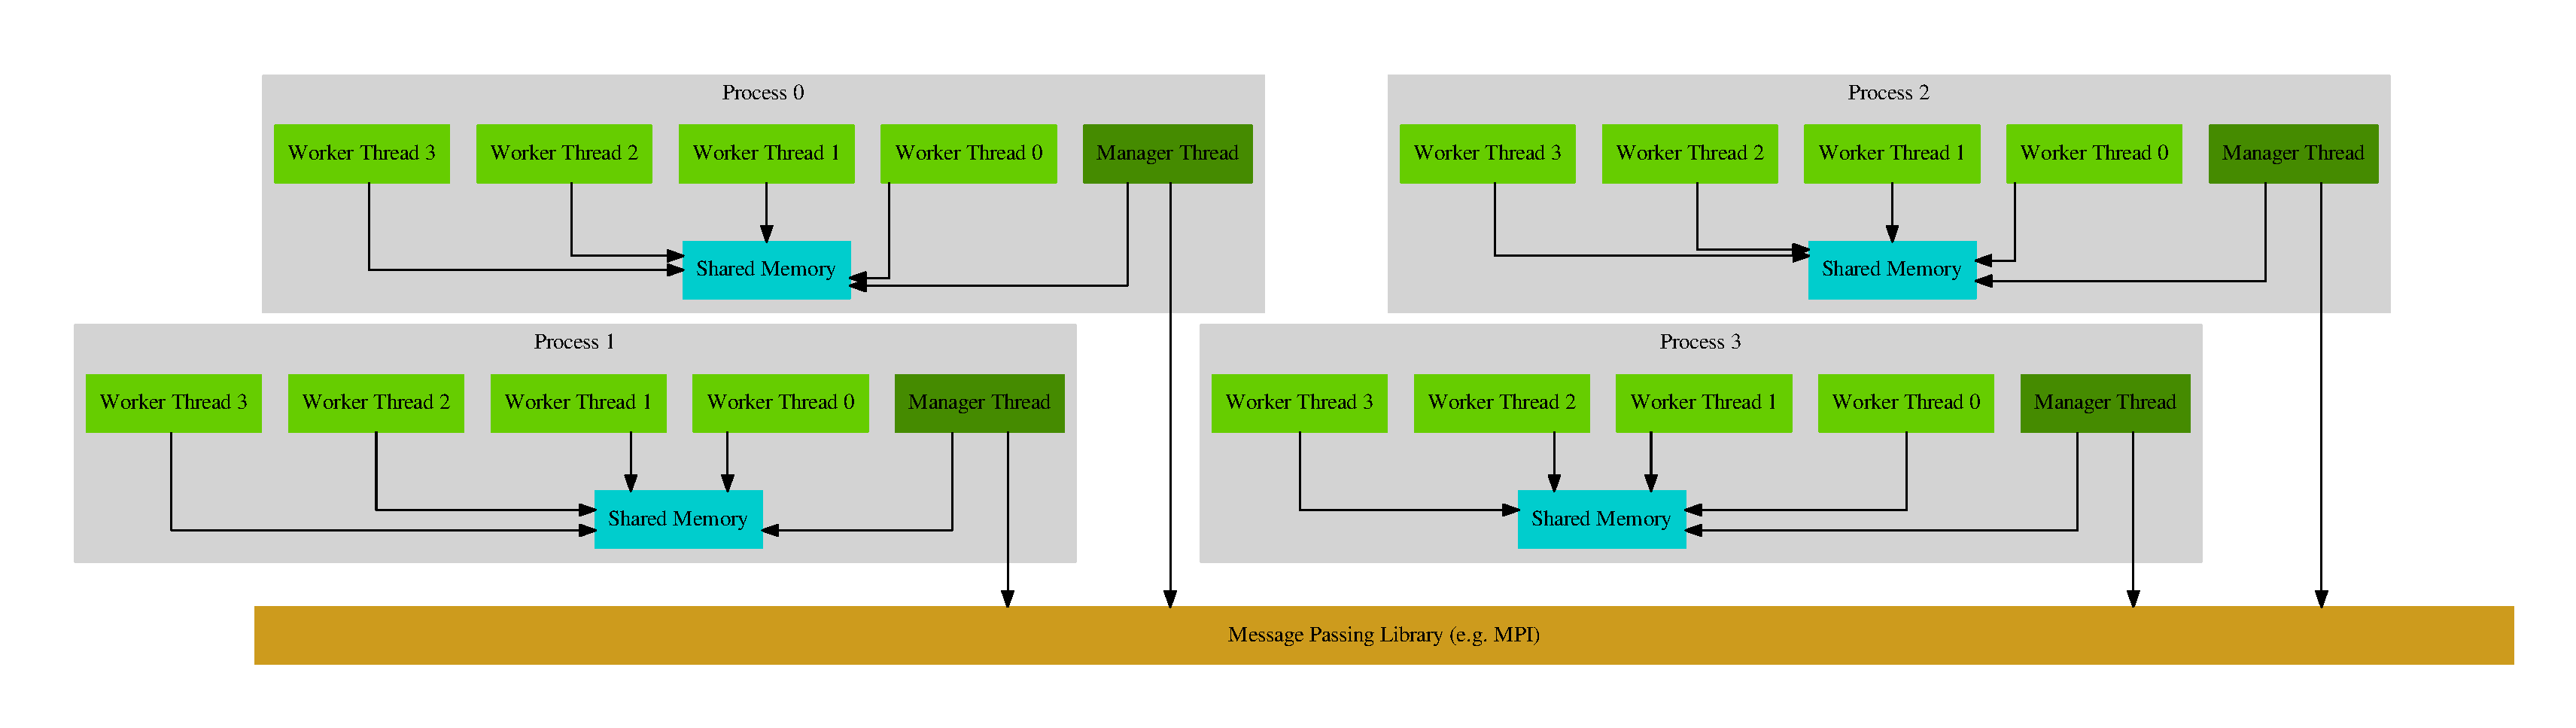
\includegraphics[width=\textwidth,quiet]{figs/graphviz/warped_communication.pdf}
    \caption{Communication Model of \textsc{warped2}}\label{warped2_communication}
\end{figure}

%% Scheduling
This communication model not only allows for high scalability and reduced communication overhead
within processes, but allows Time Warp simulations to closely follow the critical path of event
execution since the worker threads can share a scheduling data structure to process events from.  In
\textsc{warped2} this scheduling data structure is call an \emph{LTSF Queue}.  Fewer LTSF queues
creates a bottleneck since multiple worker threads cannot always access them simultaneously without
contention.  On the other hand, more LTSF queues allows higher degrees of concurrency but
complicates the scheduling of events on the critical path of execution --- triggering more rollbacks
and consequently decreasing in the event processing efficiency.

%% Partitioning and Message Aggregation
To reduce communication overheads in both message passing and shared memory communication,
partitioning of the work between processes and threads will also be explored.  Partitioning the work
in a parallel discrete event simulation is achieved by simply partitioning the LPs.  In
\textsc{warped2}, a two phase partitioning scheme will be explored.  The first phase is for
partitioning LPs among processes in order to minimize interprocess communication and the second phase
is for further partitioning the LPs in a process among LTSF queues which will localize LP
communication among worker threads, allowing better cache locality, and lowering rollbacks.  To
further reduce the side effects of message passing communication, messages that are sent to the same
process are aggregated and sent together as a single larger message.

%% GVT and Termination
The combination of shared memory and message passing communication does create some complications in
the implementation of a Time Warp system.  GVT and termination detection algorithms are usually
designed for either shared memory or message passing but not both
\cite{mattern-93,bellenot-90,fujimoto-94,xaio-95}.  Using a single message passing algorithm between
worker threads and between processes would mean that some kind of message passing scheme would have
to be implemented for worker threads to communicate.  This scheme would still use shared memory for
message communication but would also have the overheads of explicit message passing.  On the
contrary, it is possible to have a single shared memory algorithm that extends to distributed memory
systems but would require more complex algorithms that would either not scale efficiently or would
require extra synchronization and communication.  For these reasons, the GVT and termination
algorithms developed for \textsc{warped2} include both a message passing algorithm and a shared
memory algorithm that work in conjunction.  For GVT estimation, both synchronous and asynchronous
algorithms have been implemented.  The asynchronous algorithm is based on Mattern's message passing
algorithm\cite{mattern-93} and Fujimoto's shared memory algorithm \cite{fujimoto-94}, whereas the
synchronous algorithm is based on a synchronized global reduction between all threads from all
processes.  The termination detection algorithm is an asynchronous algorithm based on the ``sticky
flags'' principle\cite{mattern-91} where the state of each process is based on the state of all of
its threads.

\section{Thesis Overview}

The remainder of this thesis is organized as follows:

Chapter \ref{background} contains some background information on parallel simulation and
parallel computing that is used in this thesis.

Chapter \ref{related_work} reviews several of the prominent parallel simulation kernels
that use the Time Warp synchronization protocol.  The software architecture and target
compute platforms for each is described.

Chapter \ref{warped2_overview} introduces the software architecture and modeling API for
the \textsc{warped2} simulation kernel.

Chapter \ref{plans_of_study} provides an overview of experiments for single SMP nodes and
clusters and the models that are used in the experiments.

Chapter \ref{partitioning_communication} describes the importance of efficient message
passing communication and analyzes different approaches.  Some preliminary results are
shown and analyzed to determine the best communication model, partitioning scheme and
number of aggregated messages.

Chapter \ref{warped2_ds} describes the basic event scheduling algorithms in
\textsc{warped2} as well as the data structures used and the organization of the data
structures.  Some parameters that can be used to tune the performance of the simulation
will also be discussed.

Chapter \ref{gvt_termination} analyzes the problem of GVT and termination detection in
distributed systems and describes various algorithms that have been used as well as
algorithms used in \textsc{warped2}.

Chapter \ref{memory_management} analyzes techniques for managing memory efficiently.  A
brief overview of state saving techniques, fossil collection, and memory allocation will
be analyzed and some of the memory tuning parameters in \textsc{warped2} will be
discussed.

Finally, Chapter \ref{conclude} contains some concluding remarks and suggestions for
future research.


\chapter{Background}\label{background}

This chapter first describes some of the basics of Parallel Discrete Event Simulation (PDES) with a
focus on the Time Warp mechanism.  Then a brief overview of parallel architectures and parallel
communication models and their strengths and weaknesses are compared.  More detailed discussions are
available in the literature \cite{fujimoto-90,fujimoto-00}.

\section{Discrete Event Simulation}

Discrete Event Simulation (DES) is a method of modeling the execution of a physical system with a
sequence of events that occur at discrete time intervals \cite{law-00}.  A Discrete Event Simulation
typically contains three main data structures, namely:

\begin{description}
\item[State variables: ] A set of variables that describe the current state of the system.
\item[Simulation Clock: ] A clock to measure the progress of the simulation and determine the order
  of event processing.
\item[Pending Event Set: ] A set of future events that are waiting to be processed.
\end{description}

\noindent
A \emph{Simulation Model} describes a physical system by a set of \emph{Logical Processes} (LPs).
Each LP corresponds to a physical process that is part of the physical system.  The LPs interact
with timestamped events that dictate the simulation time that the event should be processed.  With
each event that occurs, and only when an event occurs, the state of the system is updated.

In a \emph{Sequential} Discrete Event Simulation only one event is processed at a time.  All pending
events are kept in a list that is sorted by the timestamp that the event is to be processed.  The
next event to be processed is always the one with lowest timestamp.  Each successive event updates
the state of the system, advances the simulation clock, and possibly produces new future events.
This is clearly not very efficient for large simulations.  This method can be improved by realizing
that events for different LP's are independent and will only affect the state for a single LP.

\section{Parallel Discrete Event Simulation}

\emph{Parallel} Discrete Event Simulation (PDES) is a method running a discrete event simulation on
a parallel computing platform.  The parallel computing platform can be a shared memory
multiprocessor, a distributed memory cluster, or a combination of both.  An important issue in the
design and implementation of a PDES is the \emph{synchronization mechanism} that is used to
coordinate the processing of events by the concurrently executing LPs so that they satisfy their
causal order \cite{lamport-78}.  While there are numerous synchronization mechanisms for
implementing a PDES, the technique of importance in this thesis is the Time Warp Mechanism
\cite{jefferson-85,fujimoto-90,fujimoto-00}.  The Time Warp Mechanism is an \emph{optimistic
  synchronization mechanism} where the causal ordering of events is not strictly enforced and is
sometimes (temporarily) violated by the simulation executive.  A brief overview of the Time Warp
mechanism is provided in the next subsection.

\subsection{Time Warp}

The Time Warp mechanism is an optimistic method of simulation which is based on the virtual time
paradigm \cite{jefferson-85}.  \emph{Virtual Time} provides a method of ordering events in
distributed systems which are not described by real time such as a simulation.  When used for
parallel discrete event simulation, Virtual Time is synonymous with simulation time.

In an optimistically synchronized mechanism such as Time Warp, events from different LPs are
processed independently without any consideration that lower timestamped events could be received.
Because of this, it is possible that the causal order of event is violated.  Consider the timing
diagram shown in Figure \ref{causality_violation} which illustrates this scenario with three LPs. An
event processed at $LP_1$ triggers a new event to be sent to both $LP_2$ and $LP_3$ and in turn,
$LP_3$ processes the event which triggers a new event to be sent to $LP_2$ with a lower receive time
than the previously one. If the first event received at $LP_2$ is processed before the second, then
the state could be updated and new events could be sent to other LPs incorrectly.

\begin{figure}
    \centering
    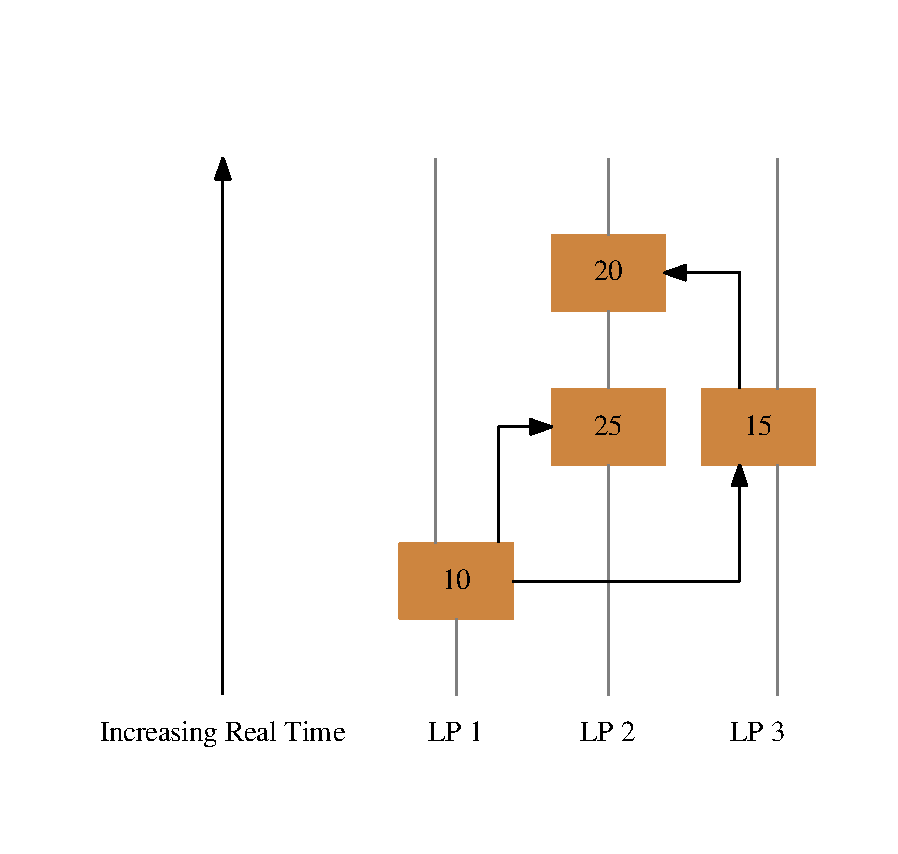
\includegraphics[width=0.4\textwidth,quiet]{figs/graphviz/causality.pdf}
    \caption{Causality Violation}\label{causality_violation}
\end{figure}

When a causality violation is detected at an LP the effects of the incorrectly processed event(s)
must be undone. The process of undoing the effects is called a \emph{rollback} and the event that
triggers a rollback is called a \emph{straggler event}. Jefferson \cite{jefferson-85} describes how
to support rollbacks by having three data structures per LP:
\begin{inparaenum}[(1)] \item Input Queue, \item Output Queue, and \item State Queue
\end{inparaenum} which are illustrated in Figure \ref{lp_data_structures}. The input queue
contains all past and future event, the output queue contains all previously sent events, and
the state queue contains snapshots of previous states.

\begin{figure}
    \centering
    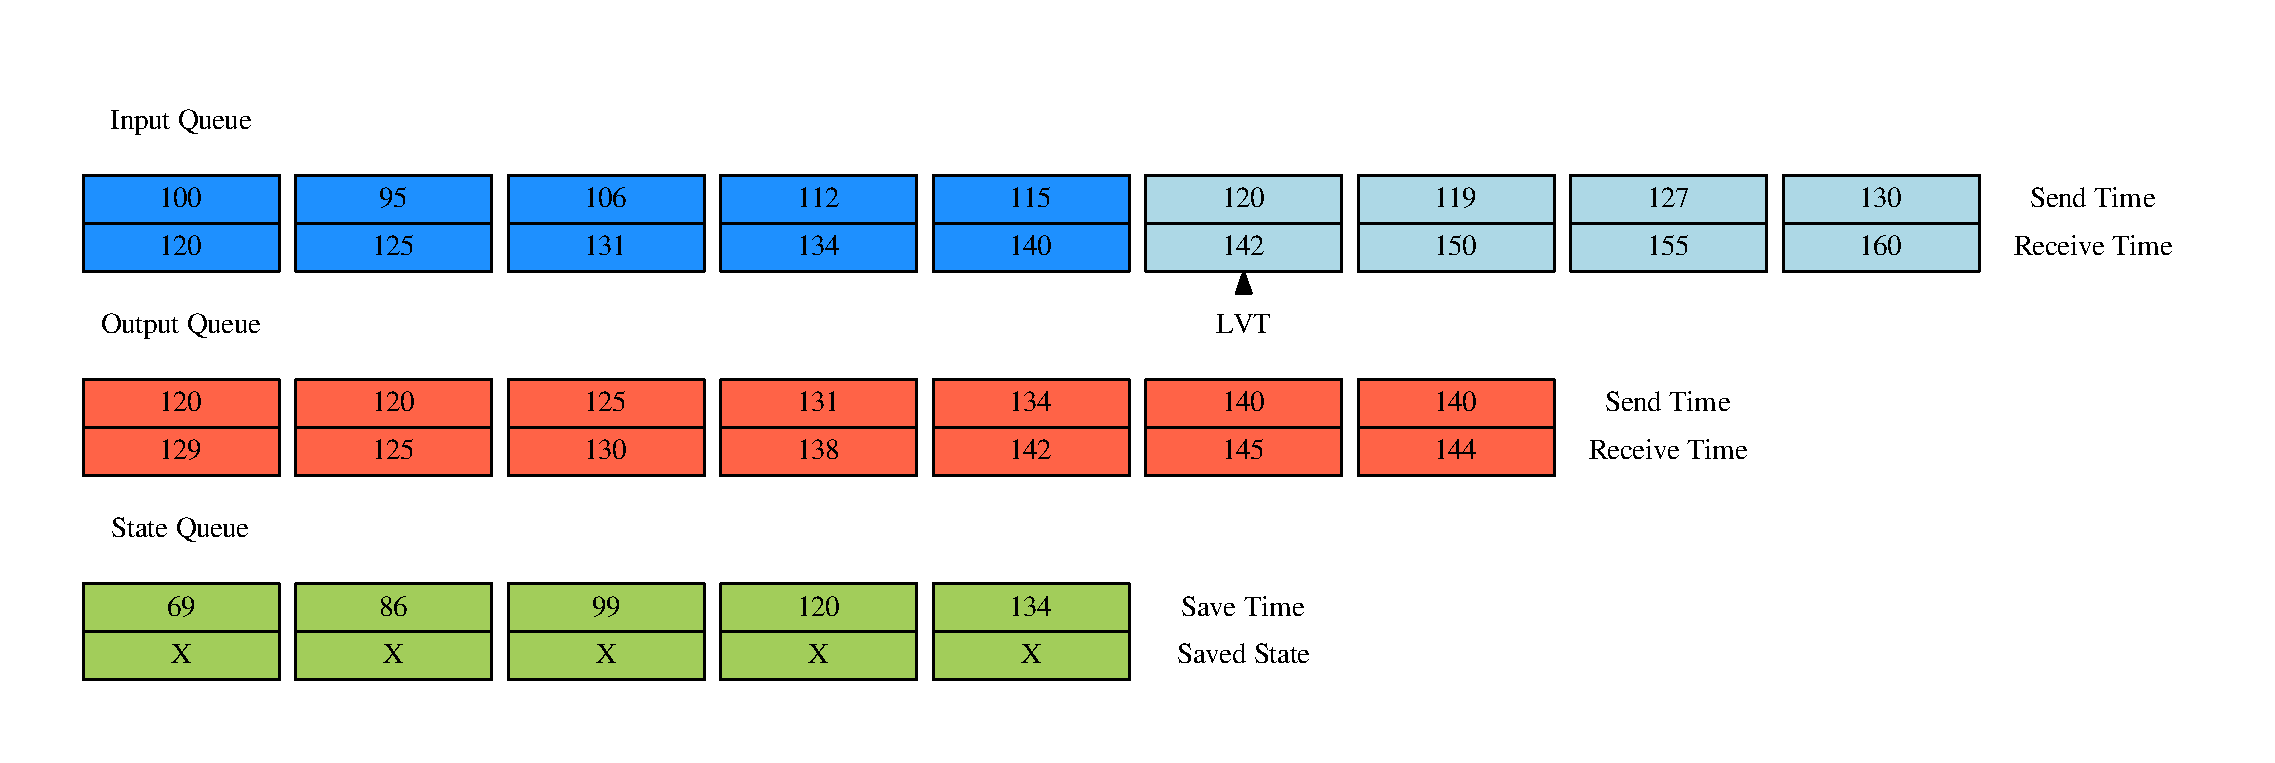
\includegraphics[width=\textwidth,quiet]{figs/graphviz/logical_process.pdf}
    \caption{Time Warp LP Data Structures}\label{lp_data_structures}
\end{figure}

When a straggler event is detected, the LPs state is restored back to a state that was saved at a
timestamp prior to the straggler event.  All events in the output queue with a send time greater
than the straggler event that were sent incorrectly are then sent again but as an
\emph{anti-message} or \emph{negative event}.  The anti-messages are exactly the same as the events
that were already sent (positive events) but must be differentiated by including a bit indicator
within the event payload.  Anti-messages are not processed by the receiving LP but serve only to
cancel out the positive counterpart in the input queue.  If the anti-message is a straggler then a
rollback occurs in the same fashion and the process occurs recursively occurs until all causality
violations are corrected.  When an anti-message causes a rollback, it is sometimes referred to as a
\emph{secondary rollback}, whereas a rollbacks triggered by a positive straggler event is a
\emph{primary rollback}.

The \emph{Local Virtual Time} (LVT) of an LP is the timestamp of the smallest unprocessed event.  By
itself, the LVT of an LP does not mean anything but is useful for determing the \emph{Global Virtual
  Time} (GVT).  The GVT of the simulation at a given point during the simulation is the minimum
timestamp of all unprocessed events and anti-messages including the events that have been sent but
not received\cite{fujimoto-94}.  Determining (more precisely, estimating) the GVT is a complex
problem and there are numerous algorithms for determining the GVT. More details and some of the
algorithms will be discussed further in Chapter \ref{gvt_termination}.  The GVT is a lower bound on
how far a rollback can occur which makes it useful in determining which events in the input and
output queues and the states in the state queue that will never be used again and can be freed as
well as committing I/O operations that cannot be undone.  The process of freeing memory and
committing I/O operations is known as \emph{fossil collection}.  Fossil collection does not have to
be based on the GVT and several other methods of fossil collection have been developed which will be
discussed more in Chapter \ref{memory_management}.

\section{Parallel Systems Architectures}

Systems that support parallel processing come in many forms \cite{culler-97,patterson-11}.  They can
generally be characterized by how processors and memories are grouped together.  A shared memory
system is a single machine which shares a common address space for all processes and can have a
either a single physical memory unit or multiple memory units.  A cluster is a system comprised of
multiple machines with separate process address spaces connected over an interconnection network.

\subsection{Shared Memory Multiprocessor Systems}

\paragraph{A Symmetric Multiprocessor (SMP)} is a type of shared memory multiprocessor
system where each processor has uniform access to a single shared memory through a common bus.  SMP
systems cannot scale very large due to increasing memory contention as the number of processors
increasing and for this reason, they usually have 8 or fewer processors.  To increase available
bandwidth in the system, each processor usually has one or two levels of private caches as well as a
shared cache which act as a way limit the number of memory accesses.  Figure \ref{smp} illustrates
what a typical SMP system might look like.

\begin{figure}
  \centering
  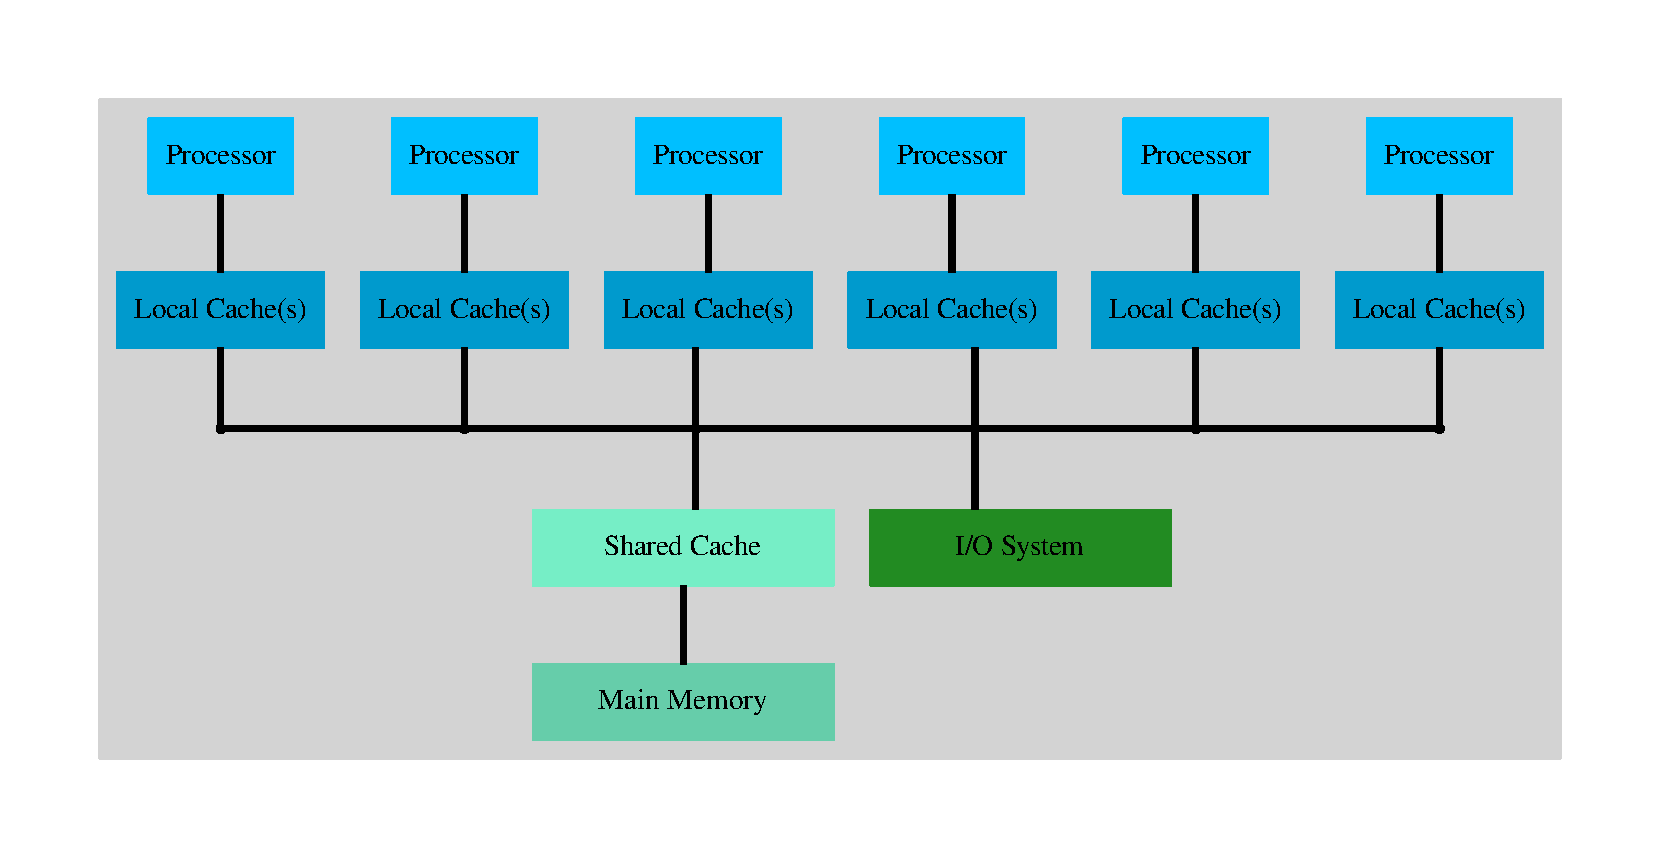
\includegraphics[width=0.75\textwidth,quiet]{figs/graphviz/smp.pdf}
  \caption{SMP System}\label{smp}
\end{figure}

\paragraph{A Distributed Shared Memory} system, also known as a Non-Uniform Memory Access
(NUMA) system has multiple memories that are distributed.  In these systems, the programming model
is as a shared memory (SMP) platform, but access to different memories may have different access
times.  In general, an interconnection network connects processors and memories together with one or
more processors per memory unit.  Because memory access times can vary, software on NUMA systems
usually try to keep memory accesses local to a processor.  However, NUMA systems can scale much
larger than SMP systems because contention to single memory does not necessarily increase with an
increasing number of processors.  Figure \ref{distributed} illustrates what a typical NUMA system
might look like.

\begin{figure}
  \centering
  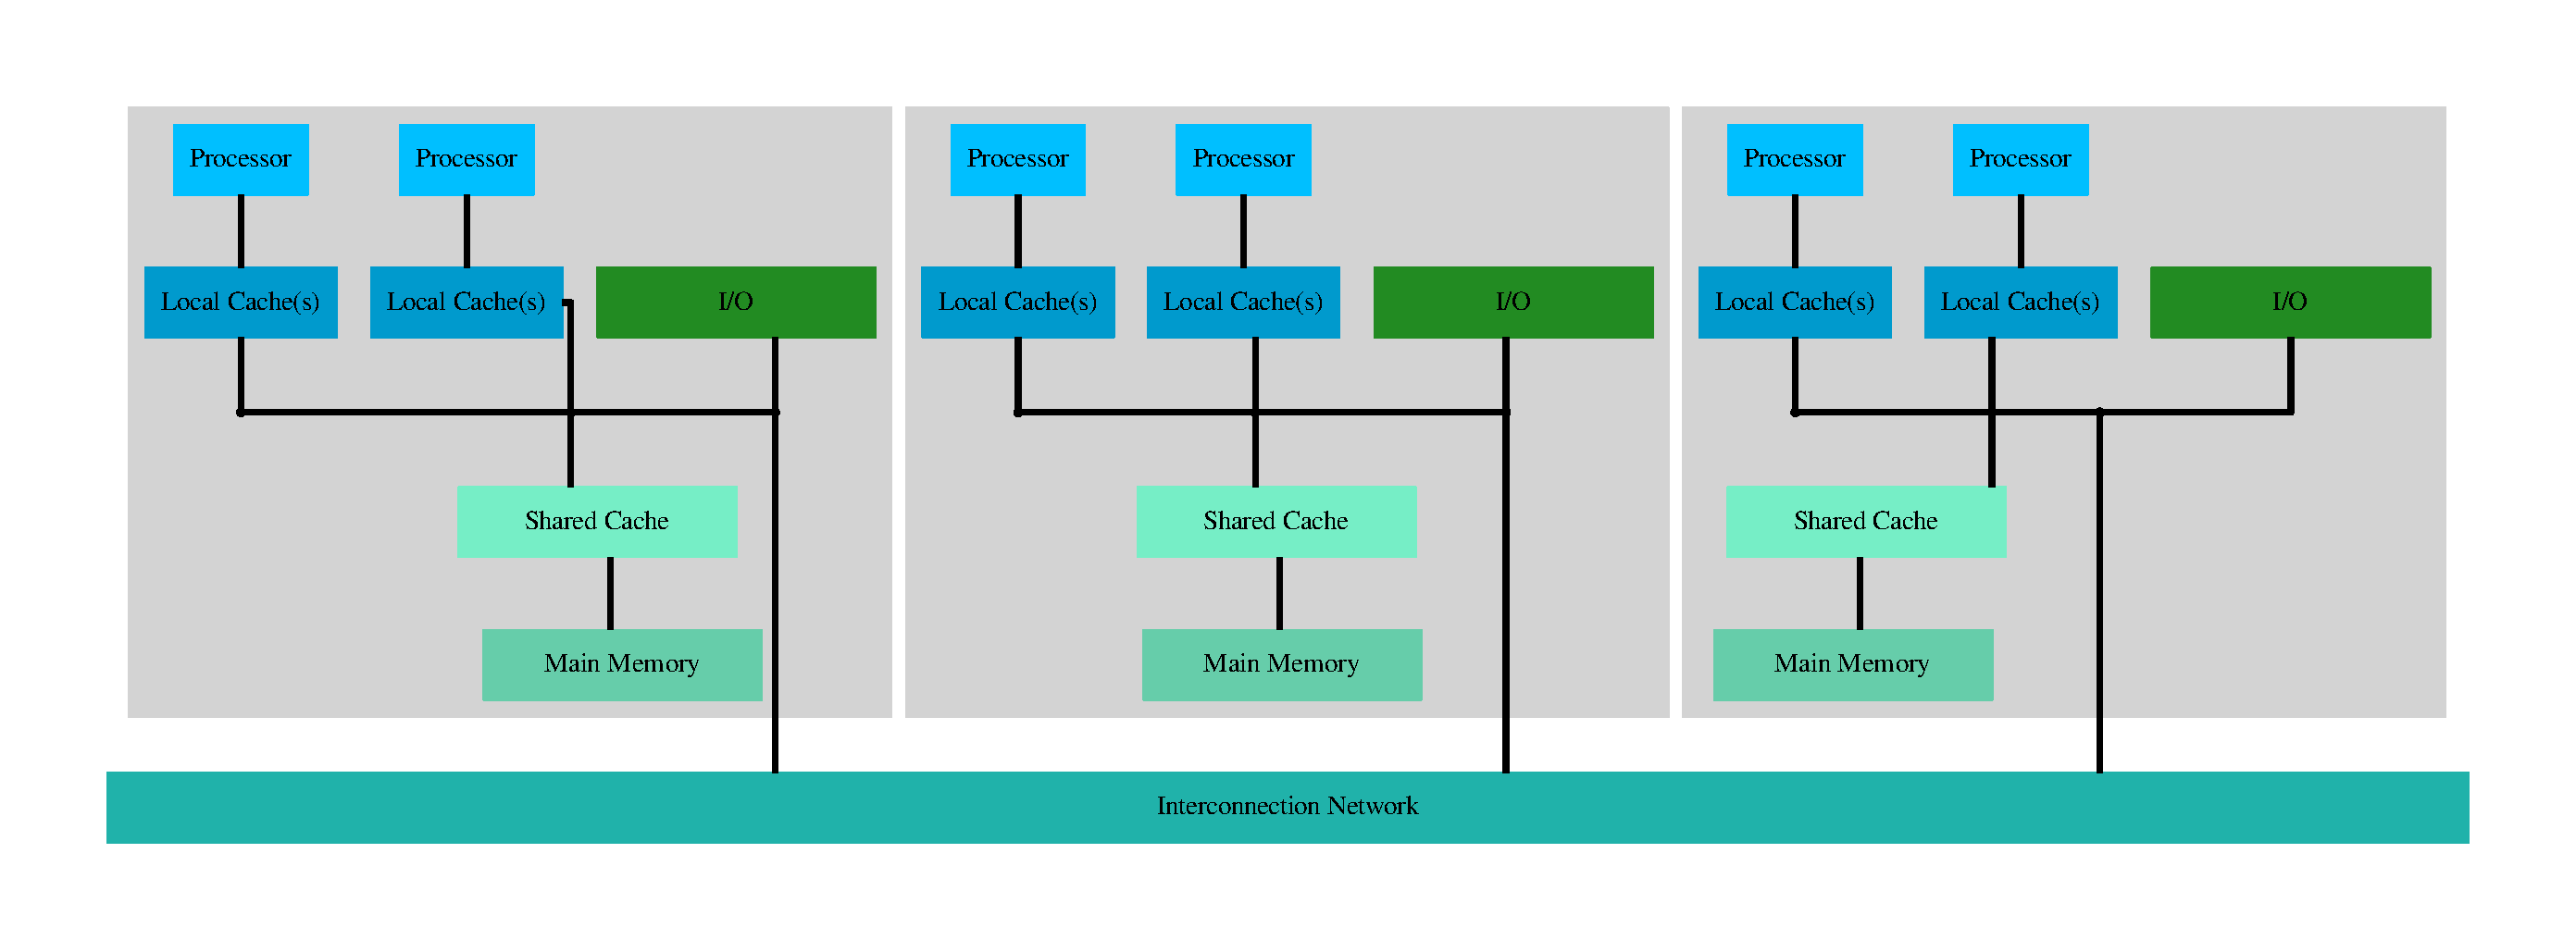
\includegraphics[width=\textwidth,quiet]{figs/graphviz/distributed.pdf}
  \caption{NUMA System}\label{distributed}
\end{figure}

\subsection{Clustered Systems}

\paragraph{A Beowulf Cluster} is a type of cluster which appears to the user as a single
machine but is actually a loosely coupled set of machines connected together over a local network.
A single program is executed by all machines concurrently by launching multiple processes on each
machine.  A program written for a beowulf cluster typically use some type of message passing to
communicate among processes and typically uses parallel communication software such as MPI or PVM.
Figure \ref{beowulf} illustrates a common realization of a beowulf cluster.

\begin{figure}
  \centering
  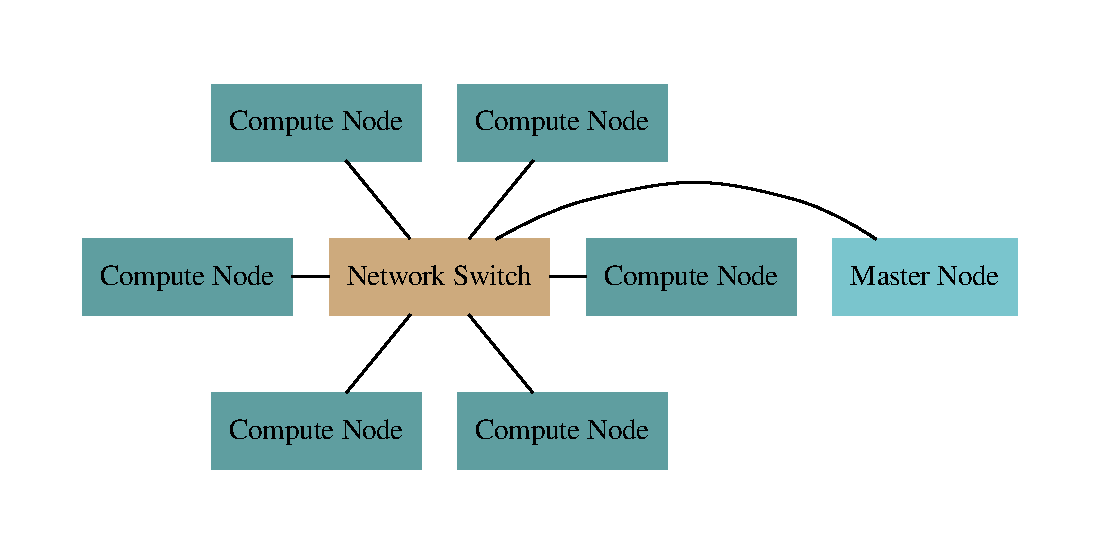
\includegraphics[width=0.6\textwidth,quiet]{figs/graphviz/beowulf.pdf}
  \caption{Beowulf Cluster}\label{beowulf}
\end{figure}

\section{Parallel Systems Communication}

Parallel applications are composed of multiple processes/threads that execute independently in
parallel and may have to exchange information.  For the following discussion, the term process will
be used although it still applies to threads as well.  Processes can communicate by either
explicitly passing messages to each other by means of well defined message formats or by using
shared data structures that all processes can access.  The former method of communication is known
as \emph{message passing} and the latter method of communication is known as \emph{shared memory}
communication.  Both communication methods are fundamentally different and both have strengths and
weaknesses.

\subsection{Message Passing}

In a message passing system, processes communicate only through serialized messages.  The formats of
the messages must be defined so that the message can be serialized and deserialized by the sender
and the receiver, respectively.  Message passing can be either synchronous or asynchronous.

With synchronous message passing, the send/receive operations for each process must be performed in
a specific order so that the sender/receiver processes operate together in a synchronized fashion.
The send operation at the sender will block until the message is received at the receiver and the
receive operation at the receiver will block until the message is fully received.  That means the
every process must follow a predictable communication pattern.  Processes cannot continue other
operations during communication operations and may slow down the whole system.

On the other hand, asynchronous communication allows processes to start a send and receive
operations and immediately continue without blocking.  To allow this, temporary queues must be used
to hold pending operations.  The processes do not have to follow a predictable communication pattern
in this case because the messages will be queued and can be processed at any time and in any order.

The main advantage of message passing, in general, is that the number of cooperating processes can
be scaled to essentially any size as long as the work is partitioned in the right way so that
communication is minimized.  Also, the processes can execute in address spaces on totally separate
machines and communicate over a local network connection.  A disadvantage, however, is the latency
introduced by the necessity to serialize, deserialize, and copy messages which can take a relatively
long time compared to the speed of computation.  Furthermore, if an interconnection network is used
between processes, an extra communication latency further slows the system down.  This makes message
passing especially hard for fine-grained parallel applications which must send and receive a lot of
small messages.  An illustration of message passing is shown in Figure \ref{communication}(a).

\subsubsection{Message Passing Interface (MPI)}

MPI \cite{gropp-94} is an extensive message passing API specification for parallel applications and
supports both synchronous and asynchronous forms of communication.  It is a standard specification
for developers and MPI users and many current implementations exist.  Two widely used
implementations of MPI are MPICH and OpenMPI.

\subsection{Shared Memory}

The processes in a parallel application can also share a common address space and communicate
through shared data structures.  A producer process will insert data directly into the data
structure and a consumer process will remove the data and use it.  This takes much less time to
transmit data than with a message passing scheme.  Furthermore, pointers can be used to eliminate
the need to copy large amounts of data.  Access to the shared data structures, however, must be
protected so that multiple processes cannot simultaneously perform read-modify-write operations on
the same data which could cause unpredictable results.  Access to the data structures is usually
enforced using lock synchronization mechanisms that protect entire sections of code that are
executed by different processes and can end up accessing the same data structures such as mutexes or
semaphores.  The performance of shared memory data structures may suffer from performance if lots of
processes contend for the lock at the same time.  For this reason, it is very hard to scale systems
that use only shared memory as a means of communication.  An illustration of a simple shared memory
system is show in Figure \ref{communication}(b).

\begin{figure}
  \begin{minipage}{.5\textwidth}
    \begin{center}
      (a)
      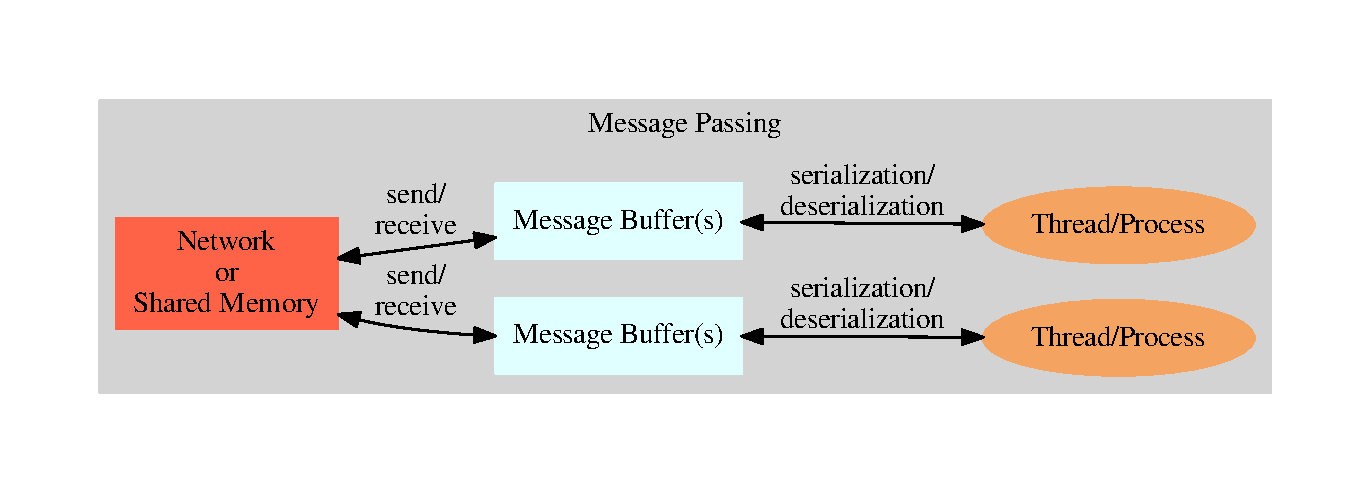
\includegraphics[width=\textwidth,keepaspectratio,quiet]{figs/graphviz/message_passing.pdf}
    \end{center}  
  \end{minipage}%
  \hfill
  \begin{minipage}{.5\textwidth}
    \begin{center}
      (b) 
      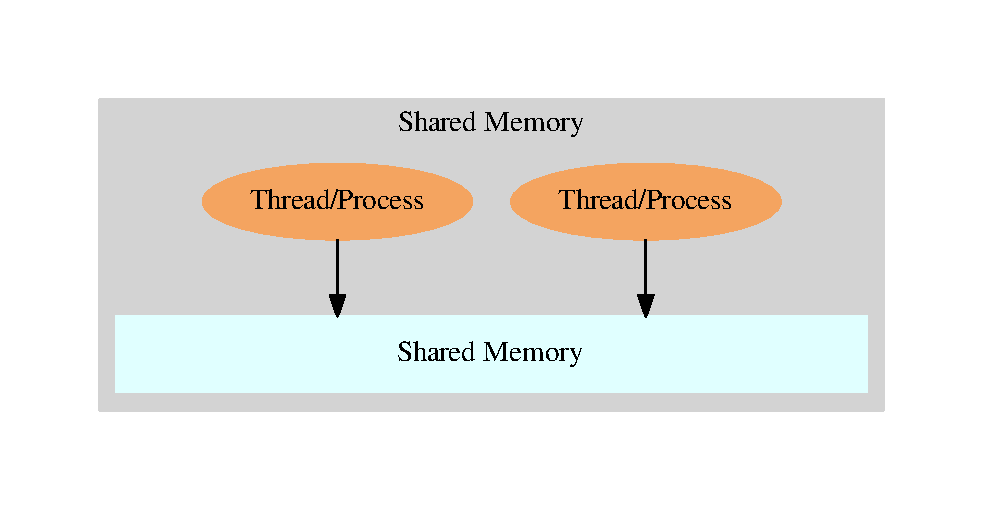
\includegraphics[width=\textwidth,keepaspectratio,quiet]{figs/graphviz/shared_memory.pdf}
    \end{center}  
  \end{minipage}
  \caption{Message Passing and Shared Memory Communication}\label{communication}
\end{figure}



\chapter{Related Work}\label{related_work}

This chapter give an overview of some of the most popular Time Warp implementations.  For each
implementation the design will be described at a high level with a focus on the target architecture.
The featured data structures and algorithms for each will also be described as well as the strengths
and weaknesses.

\section{Georgia Tech Time Warp (GTW)}

Georgia Tech Time Warp \cite{das-94} (GTW) was a general purpose Time Warp Simulator designed
specifically for shared memory multiprocessors.  It is not used anymore, however, because it was
only written to target architectures that are now obsolete such as the SparcStation and SGI
PowerChallenge.  Although GTW is not used any more, its design has influenced the design of other
simulators that are still used widely in practice.  GTW simulation models run in a single
multi-threaded processes and use only shared data structures to communicate between threads that are
bound to single processor.

All of the LPs in a simulation model are statically allocated to a single thread so that events for
an LP are always processed by the same processing core.  The pending event set is distributed among
threads with each having its own data structures for the set of LPs that are assigned to it.  Since
the threads can only run on a single processor, the data structures also belong to a single
processor.  The pending event set for each processor consists of three main data structures listed
below\cite{das-94}:

\begin{enumerate}
\item The \emph{Message Queue} is a linked list that contains positive messages that are destined
  for the LPs mapped to the owning processor.  Access to the message queue must be synchronized
  because it can be accessed by tasks running on any processor.
\item The \emph{Cancel Queue} is a linked list that serves exactly the same purpose as the message
  queue except that it contains only negative messages(anti-messages).  Access to this queue must
  also be synchronized.
\item The \emph{Event Queue} is used to hold unprocessed and processed events and is directly used
  to schedule events to be processed.  The event queue is actually made up of different data
  structures, one for processed events and one for unprocessed events.  The processed events are
  contained within a doubly linked list and the unprocessed events are contained within a priority
  queue which can be configured to be either a calendar queue or a skew heap depending on a user
  configuration.
\end{enumerate}

\noindent
When messages are sent between LPs, they are inserted directly in the message queue or the cancel
queue depending on whether they are positive or negative.  Each thread processes events by first
moving events from the message queue to the event queue and processing rollbacks.  Then, the
messages from the cancel queue are removed and cancellations are processed and any more rollbacks
are processed.  One or more of the smallest events from the event queue are then processed and added
to the processed event list.  This procedure is repeated over and over again by all processors.
Pseudocode for the main event processing loop in GTW is show in Figure \ref{gtw_processing}.

\begin{algorithm}
\DontPrintSemicolon
    \While{eventQ is not empty} {
        move messages from MsgQ to EvQ and process any rollbacks\;
        remove anti-messages from CanQ, process annihilations and rollbacks\;
        remove N smallest timestamped events E from EvQ\;
        process the N events\;
    }
\caption{GTW Main Event Processing Loop\cite{das-94,fujimoto-94}\label{gtw_processing}}
\end{algorithm}

\noindent
To avoid accessing the message queues and cancel queues too often, which is a contention point, a
larger value of N can be used.  GTW calls this batch processing and N is the batch interval.  With
batch processing, multiple events will be processed at a time without processing any rollbacks or
cancellations.

Since GTW is only uses shared memory communication, anti-messages do not need to be
explicitly sent.  Only a pointer to the event that needs to be cancelled is necessary.
Fujimoto calls this method \emph{direct cancellation}.  Also by only using shared memory,
GVT can be calculated very quickly using shared data structures instead of passing
messages around to all processors.  The downfall of GTW, however is that it was limited to
only a single multiprocessor machine and it was only designed and optimized for specific
architectures.

GTW also imposed some unnecessary requirements for the developer of particular simulation models.
The partitioning of the LPs among processors must be done in the simulation model during
initialization.  That means that the model developer must understand some the features of the
underlying architecture such as the number of processors, to effectively partition the LPs.
Furthermore, the initial partitioning of the LPs is hard to dynamically balance during the
simulation because there are no separate input queues for each LP but rather a single message queue
to hold all unprocessed events for each processor.

\section{Clustered Time Warp (CTW)}

Clustered Time Warp \cite{avril-95} (CTW) uses a hybrid sequential/time-warp approach by processing
events within a \emph{cluster} of LPs sequentially and using the Time Warp mechanism between the
clusters.  This design was chosen because it works well for digital logic simulation which tend to
have localized computation within a group of LPs.  Furthermore, digital logic simulation tends to
have low computational granularity and lots of LPs which can lead to a significant number of
rollbacks and a large memory footprint in a traditional Time Warp simulator.  CTW is implemented for
shared memory multiprocessors but only uses shared memory for use with a custom message passing
system so that it can better support NUMA architectures.  It is not designed for use on a Beowulf
Cluster.

Each cluster of LPs has a timezone table, an output queue, and a set of LPs that each have an input
queue and a state queue.  The timezones in the timezone table are divided by timestamps of the
events received from LPs on different clusters.  Whenever an event is received from a remote
cluster, a new timezone is added.  Only a single output queue is needed per cluster because
anti-messages can only be sent between clusters and not between LPs on the same cluster.

When a straggler event arrives at a cluster, all of the LPs that have processed events with
timestamps greater than the straggler event will be rolled back.  This rollback scheme is called
\emph{clustered rollback}.  The alternative to clustered rollback is \emph{local rollback}.  In a
local rollback scheme the straggler event would be inserted into the receiver LPs input queue and
the LP will roll back when it is detected.  Although clustered rollbacks may cause some LPs to be
rolled back unnecessarily leading to slower computation, the approach was chosen for CTW because
processed events will not have to be saved which requires less memory.

CTW uses a form of infrequent state savings with the timezone table used to determine the frequency.
When an event is about to processed for an LP, the timezone of the last processed event is looked up
and if event that is about to be processed is in a different timezone then the state is saved.  This
approach in which all LPs save their state every time an event is processed in a new timezone
regardless of whether it receives an event from a remote cluster is called \emph{local
  checkpointing}.  This method reduces the state saving frequency more than a \emph{clustered
  checkpointing} approach in which only the LP that receives an event from a remote cluster saves
its state.  The local checkpointing approach was chosen for CTW because a larger state saving
frequency can increase rollback computation and it can even lead to more memory consumption because
more events must be saved for coast forwarding during state restoration.

\section{Rensselaer's Optimistic Simulation System (ROSS)}

Rensselaer's Optimistic Simulation System \cite{carothers-00} (ROSS) is a general purpose simulator
that is capable of running both conservatively and optimistically synchronized parallel simulations
as well as sequential simulations.  It is most often used for optimistic parallel simulations which
is implemented with the Time Warp mechanism.  ROSS started as a reimplementation of GTW and is still
modeled after it but has had many enhancements.  The same basic event scheduling mechanism is used
but ROSS supports different priority queue implementations and different algorithms are used for
fossil collection, state saving, and GVT calculation.  In addition, ROSS uses processes instead of
threads and uses message passing explicitly with MPI instead of shared memory for communication
among the processes.

Just as in GTW, ROSS maps every LP to a process and each process contains its own pending event set
structures.  No locks are needed explicitly within each process because there are no shared data
structures among processes.  The data structures are very similar to those used in GTW but have a
different naming convention.  The main data structures in ROSS are:

\begin{enumerate}
\item The \emph{Event Queue} is analogous to the message queue in GTW.  It contains the positive
  events for all LPs in the corresponding process.  In addition, an event queue is used to hold all
  remote events regardless of whether it is positive or negative.  The event queue is implemented as
  a linked list.
\item The \emph{Cancel Queue} is a linked list which is used to hold negative events for all LPs for
  the corresponding process.  The cancel queue is used in the exact same way as GTW except that no
  locks are necessary.
\item The \emph{Priority Queue} is analogous to the unprocessed event queue in GTW and contains
  events in timestamp order.  ROSS also allows the priority queue to be implemented as a calendar
  queue, heap, splay tree, or AVL tree depending on user configuration.
\end{enumerate}

To reduce the time taken to fossil collect LPs, ROSS further divides the LPs in a single process
into groups called Kernel Processes (KPs).  All LPs in a KP are rolled back together and fossil
collected together in a similar manner as a clustered rollback in CTW.

ROSS also uses reverse computation \cite{carothers-99} to rollback LPs to a previous state instead
of using the traditional copy state saving.  This method allows simulations to potentially run in a
smaller memory footprint because the previous states of LPs are not required to be saved.

\section{\textsc{warped}}

\textsc{warped} \cite{martin-96,ramanan-98-iscope} is the predecessor of \textsc{warped2} and serves
as the basis for the design and architecture of \textsc{warped2}.  \textsc{warped}, unlike the
previous Time Warp simulators, follows Jefferson's classic model with LPs having their own input,
output, and state queues.  It started as a completely process based solution with only message
passing for communication, but eventually, with the development of multicore processors, each
process was extended into multiple threads to further enhance concurrent processing of events.  Over
the years, though, with many researchers developing new algorithms, the complexity of
\textsc{warped} became unmaintainable.  A great deal of indirection which, although made for a super
configurable and modular design, became too complex for new developers to learn and enhance it.
This has led to the development of \textsc{warped2} which is detailed throughout the remained of
this document.

\section{Others}

\subsection{The ROme OpTimistic Simulator (ROOT-Sim)}

The ROme OpTimistic Simulator \cite{pellegrini-11} (ROOT-Sim) is another general purpose Time Warp
Simulator that uses message passing via MPI.  Like \textsc{warped}, ROOT-Sim is a more classic Time
Warp implementation with each LP having their own input, state and output queues.  What sets
ROOT-Sim apart from other Time Warp simulators is the internal instrumentation tool, Dynamic Memory
Logger and Restorer (DyMeLoR) that can optimize memory usage.  DyMeLoR can determine whether the
simulation models are better fit for copy-state saving or incremental state saving and transparently
switch between them during runtime.  Another service that ROOT-Sim offers is the Committed and
Consistent Global Snapshot (CCGS).  After each GVT calculation, ROOT-Sim transparently rebuilds a
global snapshot of all LP states.  Each LP can access its portion of the global snapshot on every
GVT calculation.  With this service, a simulation model can implement any custom global snapshot
algorithm.

\subsection{ROSS-MT}

ROSS-MT \cite{jagtap-12} is a multi-threaded version of ROSS which is optimized to use shared memory
to communicate among threads.  The use of message passing with MPI was completely removed and all
events are sent by direct insertion into the event queues.  To reduce the added contention on the
event queues, they are further divided by possible senders.  ROSS-MT also optimizes the memory
management so that it is more NUMA aware.



\chapter[\textsc{warped2}]{The \textsc{warped2} Simulation Kernel}\label{warped2_overview}

\textsc{warped2} is a discrete event simulation kernel that has been designed primarily for research
explorations with Time Warp synchronized parallel simulation on multi-core processors and clusters.
The \textsc{warped2} system is implemented in C++ and presents a modeling API to assist in model
development.  That said, the API is fairly low-level and does include some concepts that exist
specifically to support the Time Warp implementation (\emph{e.g.,} state definition and copy
constructors for the state).  The \textsc{warped2} system is stored in git repositories at
\url{https://github.com/wilseypa/warped2} and \url{https://github.com/wilseypa/warped2-models}.  The
\url{warped2} repository contains two implementations of the API, namely: (i) one providing
sequential simulation capabilities, and (ii) one providing a Time Warp synchronized parallel
simulation capability.  The \url{warped2-models} repository (currently) contains 4 simulation models
that can be used to exercise the simulation kernel.  Detailed descriptions of the models are
available in the README of the repository.

The remainder of this chapter provides a brief overview of the \textsc{warped2} simulation model API
and the Time Warp implementation.  In each case, a high level overview is first presented and then a
detailed discussion of the C++ classes and object interactions is reviewed.  A complete example of
an airport model implementation is also provided in appendix \ref{airport_model}.

\section{The \textsc{warped2} Modeling API}

\subsection{Conceptual Overview}

\begin{figure}
    \centering
    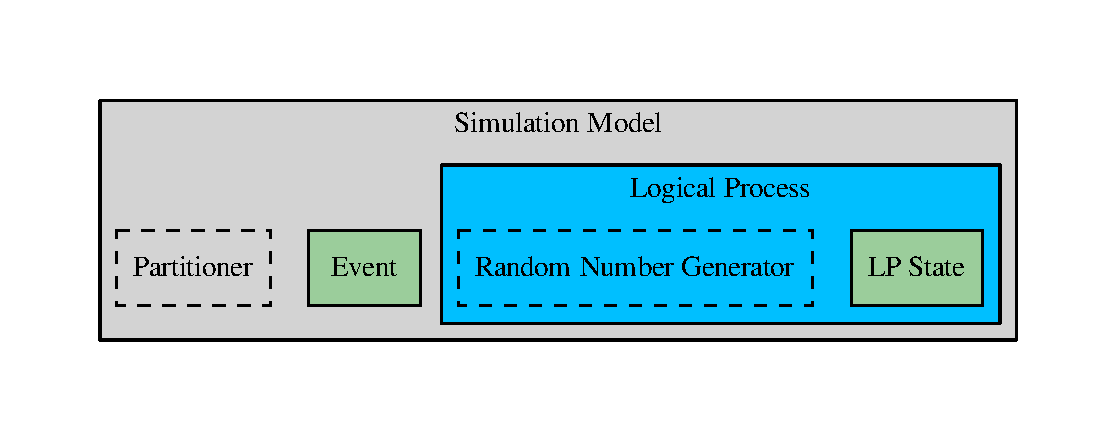
\includegraphics[width=\textwidth,quiet]{figs/graphviz/model.pdf}
    \caption{Overview of a \textsc{warped2} Simulation Model}\label{warped2_conceptual_overview}
\end{figure}

In general, \textsc{warped2} represents a discrete event simulation as a collection of \emph{Logical
  Processes} (LPs) that process and exchange \emph{events}.  The LPs are each discrete event
processing subsystems that process and exchange events with other LPs.  This model follows closely
the general PDES simulation model for optimistically synchronized parallel simulation
\cite{fujimoto-90,jefferson-85}.  An illustration of the main components in a \textsc{warped2}
simulation model is presented in Figure \ref{warped2_conceptual_overview}.  The Partitioner object
and Random Number Generator objects are optional depending on the needs of the model.  A brief
overview of these components follows.

At its most basic level, a simulation model in \textsc{warped2} must contain a definition of an
\texttt{event} and a definition for one more types of \texttt{logical processes (LPs)}.  For
each LP type, the user must define the state of the LP and construct a description of what it
means to process an event.  While this is the minimalist requirements for the construction of
a \textsc{warped2} simulation model, most models will require two more items, namely:
\begin{inparaenum}[(1)] \item declarations of rollbackable random number generators and,
at the user's discretion, \item the definition of a Partitioner object to make LP assignments
to some number of processes/threads.\end{inparaenum}

If an LP requires \emph{random number generation}, the user will also have to instantiate a Random
Number Generator object that can save and restore its internal state (this is needed so that the
generator will always produce the same sequence of random numbers even in the presence of
rollbacks).  Fortunately, the C++11 standard libraries contain generators that are all easily setup
to support rollback.  The details on how to achieve this is presented in the next section.

Finally, the simulation modeler may decide to implement a custom partitioner to assign the LPs to
specific processing locations.  The default kernels of \textsc{warped2} contains three partitioners.
The first two are general purpose round robin partitioners; one sequentially walks the list of LPs
and assigns each LP to the next partition.  The second round robin partitioner assigns LPs in equal
sized blocks to the partitions.  While the second partitioning method is only nominally distinct
from the first, we have discovered that modelers tend to build models such that frequently
communicating LPs are instantiated in sequence and the resulting performance results from the block
scheduled LPs is, in general, much better.  The third partitioner is a profile driven partitioning
mechanism that attempts to minimize the number of events that are exchanged by LPs in different
partitions.  Briefly a user must first pre-simulate the simulation model with the sequential
\textsc{warped2} kernel with event tracing turned on.  This causes event information to be recorded
into a file that is then used by the subsequently invoked parallel simulation to make the LP
assignments.

\subsection{The C++ Modeling API of \textsc{warped2}}

The modeling interface of \textsc{warped2} is a set of abstract base classes that contain methods to
be implemented in a derived class in the simulation model.  The three main base classes are
\texttt{LogicalProcess}, \texttt{LPState}, and \texttt{Event}.  A \textsc{warped2} simulation model
will need to instantiate derived classes from each of these base classes.  In addition, the user may
desire to create a custom partitioner from the \texttt{Partitoner} base class (as per the discussion
above).  In the remainder of this section, each class is described in more detail and sample
implementations are shown for each.

\subsubsection{The LPState Structure}

The LPState structure is derived from by using the \texttt{WARPED\_DEFINE\_LP\_STATE\_STRUCT} macro
instead of the standard C++ syntax.  By using this macro, a \texttt{clone} method and
\texttt{restoreState} method are automatically defined to allow copy construction and copy
assignment, respectively, from a pointer to base class.  The \textsc{warped2} kernel can then save a
copy of the state and restore the state for the model without knowing the details of the state
definition.  A simple example of a LP state that contains just message counts is shown below in
Listing \ref{example_state}.

\begin{lstlisting}[caption=Example \textsc{warped2} State Definition, label=example_state, float]
WARPED_DEFINE_LP_STATE_STRUCT(ExampleState) {
    unsigned int messages_received_;
};
\end{lstlisting}

The default copy constructor and default copy assignment operator will only perform shallow copies,
so if more complex states are necessary in the model then custom implementations may be necessary.
The copy constructor will define the behavior for saving the state whereas the copy assignment
operator will define the behavior for restoring the state.  Note that the copy assignment operator
will probably not be needed since a shallow copy will usually suffice for restoring the state.

\subsubsection{The Event Class}

The \texttt{Event} base class is used as the basis for creating model specific events.  The model
must implement at least two methods: \begin{inparaenum}[(1)] \item \texttt{receiverName()} and 
\item \texttt{timestamp()} \end{inparaenum} so that the name of the receiver and receive time can be
used for ordering events from pointer to the base class.  In addition, any other data that must be
exchanged between LPs must also be included as a class member.  It is also the responsibility of the
model developer to ensure that events are serializable.  The requirement for serializable events is
needed so that they can be sent and received through the message passing system.  Additional details
regarding event serialization will be discussed in the next section.  A basic example of an event
definition is shown below in Listing \ref{event_example}.

\begin{lstlisting}[caption=Example \textsc{warped2} Event Definition, label=event_example, float]
class ExampleEvent : public warped::Event {
public:

    const std::string& receiverName() const { return receiver_name_; }
    unsigned int timestamp() const { return time_stamp_; }

    std::string receiver_name_;
    unsigned int timestamp_;

    WARPED_REGISTER_SERIALIZABLE_MEMBERS(cereal::base_class<warped::Event>(this),
                                         receiver_name_, timestamp_)
};
WARPED_REGISTER_POLYMORPHIC_SERIALIZABLE_CLASS(ExampleEvent)
\end{lstlisting}

\subsubsection{The LogicalProcess class}

The most important class definition in the simulation model is the \texttt{LogicalProcess} class.
The implementation of the \texttt{LogicalProcess} class defines the callback functions that the
\textsc{warped2} kernel interfaces with during a running simulation and thus defines the behavior of
the simulation model.  The user must include a single \texttt{LPState} as a data member of the
\texttt{LogicalProcess} and provide three callback functions:

\begin{enumerate}
    \item The \texttt{initializeLP} method is called to perform any initializations of an LP that
      must be done prior to the start of the simulation.  Initializations should include but are not
      limited to \begin{inparaenum}[(1)] \item registering a random number generator with the
        \textsc{warped2} kernel and \item producing a set of initial events to be sent.
        \end{inparaenum}
    \item The \texttt{receiveEvent} method is called when an LP is to receive an event which is
      passed by a single parameter.  The implementation of this method should process the event by
      updating the state of the LP and returning a set of new events with \emph{future} timestamps.
      If necessary, the future event timestamps should also be calculated by using the received
      event timestamp as a lower bound.
    \item The \texttt{getState} method provides a way for the \textsc{warped2} kernel to get the
      current state of the LP so that it can be saved.
\end{enumerate}

\noindent
It is necessary that there is at least one case where \texttt{initializeLP} returns an initial event
so that at least one LP instance produces an event and the simulation can start.  Otherwise the
simulation will terminate immediately. However, most simulation models will start by sending a fixed
number of events for each LP and each received event that is processed will trigger a single new
event to be sent. An example of a \texttt{LogicalProcess} implementation is shown below in listing
\ref{lp_example}.

\begin{lstlisting}[caption=Example \textsc{warped2} LogicalProcess Definition, label=lp_example, float]
class ExampleLP : public warped::LogicalProcess {
public:

    warped::LPState& getState() { return this->state_; }

    std::vector<std::shared_ptr<warped::Event> > initializeLP() override {
        this->registerRNG(this->rng_);
        std::vector<std::shared_ptr<warped::Event> > initial_events;

        /* Create new event(s) and insert into initial_events vector */

        return initial_events;
    }

    std::vector<std::shared_ptr<warped::Event>> receiveEvent(const warped::Event& event) {
        ++this->state_.messages_received_;
        std::vector<std::shared_ptr<warped::Event> > response_events;

        /* Create new event(s) and insert into response_events vector */

        return response_events;
    }

    ExampleState state_;
};
\end{lstlisting}

\subsubsection{The Partitioner class}\label{partitioner}

The \textsc{warped2} kernel provides a set of default partitioners that a modeler can use.  However,
\textsc{warped2} also provides facilities so that the model developer can define a model specific
partitioner.  The user must derive from the Partitioner base class and implement just a single
\texttt{partition} method which takes as input arguments (i) a vector of all LPs and (ii) the number
of partitions desired and returns a vector of vectors of LPs corresponding to the partitions and the
LPs within each partition.  In general, the partitioner should work for any number of partitions and
not impose any constraints.  A simple example of a partitioner is shown in listing
\ref{partitioner_example}.

\begin{lstlisting}[caption=Example \textsc{warped2} Partitioner Definition, label=partitioner_example, float]
class ExamplePartitioner : public Partitioner {
    std::vector<std::vector<LogicalProcess*>>
    partition(const std::vector<LogicalProcess*>& lps, const unsigned int n) {

        std::vector<std::vector<LogicalProcess*>> parts(n);
        
        /* Allocate LPs from "lps" into one of the n partitions */

        return parts;
    }
};
\end{lstlisting}

\subsubsection{Random Number Generation}

If the simulation model must uses random number generators, then they must all be registered with
the \textsc{warped2} kernel so that the state of the random number generator can be saved and
restored in case of rollbacks and provide deterministic result.  The random number generators can be
any type as long as they implement the \texttt{<< operator} and \texttt{>> operator} to allow the
kernel to save and restore the internal state of the random number generator.  The random number
generators in the C++11 standard libraries \cite{c++11-rng} all fit this requirement so it is not
necessary to define a custom random number generator although it is still an option.  To register
the random number generator, the \texttt{registerRNG} template function is provided as a member of
the \texttt{LogicalProcess} class.  Any random number generators should be a data member of the
\texttt{LogicalProcess} definition so that each LP instance has its own and they should be
registered in the \texttt{initializeLP} callback function as shown in listing \ref{lp_example}.

\subsubsection{The Main Function}

Once all the necessary structures and classes have been defined, the model's main entry point
location must be implemented.  This is where all objects are instantiated and the model interfaces
with the \textsc{warped2} kernel. The model interfaces through an instance of the
\texttt{Simulation} class.

If the simulation model requires model specific command line arguments, they must be registered with
\textsc{warped2}.  This should be done before anything else is done so that the command line
arguments can be displayed without running a simulation.  \textsc{warped2} uses a third-party
library called TCLAP for command line arguments.  More details about the TCLAP library can be found
at \url{http://tclap.sourceforge.net/manual.html}.

After setting up the command line arguments, all of the LP objects and optionally a partitioner
object is created and passed to the kernel through the \texttt{simulate} method of the
\texttt{Simulation} class.  Two versions of the \texttt{simulate} method are available, one for a
model with a model specific partitioner and one without.  The type signatures for these two methods
are:

\begin{enumerate}
    \item \begin{verbatim} void simulate(const std::vector<LogicalProcess*>& lps); \end{verbatim}
    \item \begin{verbatim} void simulate(const std::vector<LogicalProcess*>& lps,
                std::unique_ptr<Partitioner> partitioner); \end{verbatim}
\end{enumerate}

\noindent
An example implementation of a models main function is shown in listing \ref{main_sample}.

\begin{lstlisting}[caption=Exmple \textsc{warped2} Main Definition, label=main_sample, float]
int main(int argc, const char **argv) {
    unsigned int num_lps = 10000;

    TCLAP::ValueArg<unsigned int> num_lps_arg("o", "lp-count", "Number of lp's", false,
                                              num_lps, "unsigned int");
    std::vector<TCLAP::Arg*> cmd_line_args = {  &num_lps_arg };
    warped::Simulation simulation {"Example Simulation", argc, argv, cmd_line_args};

    num_lps = num_lps_arg.getValue();
    std::vector<ExampleLP> lps;
    for (unsigned int i = 0; i < num_lps; i++) {
        std::string name = std::string("LP_") + std::to_string(i);
        lps.emplace_back(name, 1, i);
    }

    std::vector<warped::LogicalProcess*> lp_pointers;
    for (auto& lp : lps) {
        lp_pointers.push_back(&lp);
    }
    simulation.simulate(lp_pointers);

    return 0;
}
\end{lstlisting}


\section{The Time Warp Implementation of \textsc{warped2}}

\subsection{Conceptual Overview}

The \textsc{warped2} simulation kernel uses a modular design to make it more configurable,
extendable, and maintainable.  All components are configured and created at startup individually
and subcomponents are accessed through pointers.  Furthermore, \textsc{warped2} is written in
C++ so each component can also be an object of derived subclass that implement a well-defined
interface by a base class.  The main central component is the event dispatcher which is responsible
for calling the LP callback methods that are implemented in the simulation model during
the course of the simulation.  The event dispatcher can be configured for sequential simulation
or a Time Warp simulation.  The sequential simulation does not depend on any other components and
contains only a single list of unprocessed events.  The Time Warp event dispatcher on the other
hand depends on multiple components that implement specialized algorithms for event scheduling,
state saving, cancellation, GVT, termination, interprocess communication, and statistics.  The
main components for Time Warp and how they depend on each other are illustrated in Figure
\ref{warped2_architecture}.

\begin{figure}
    \centering
    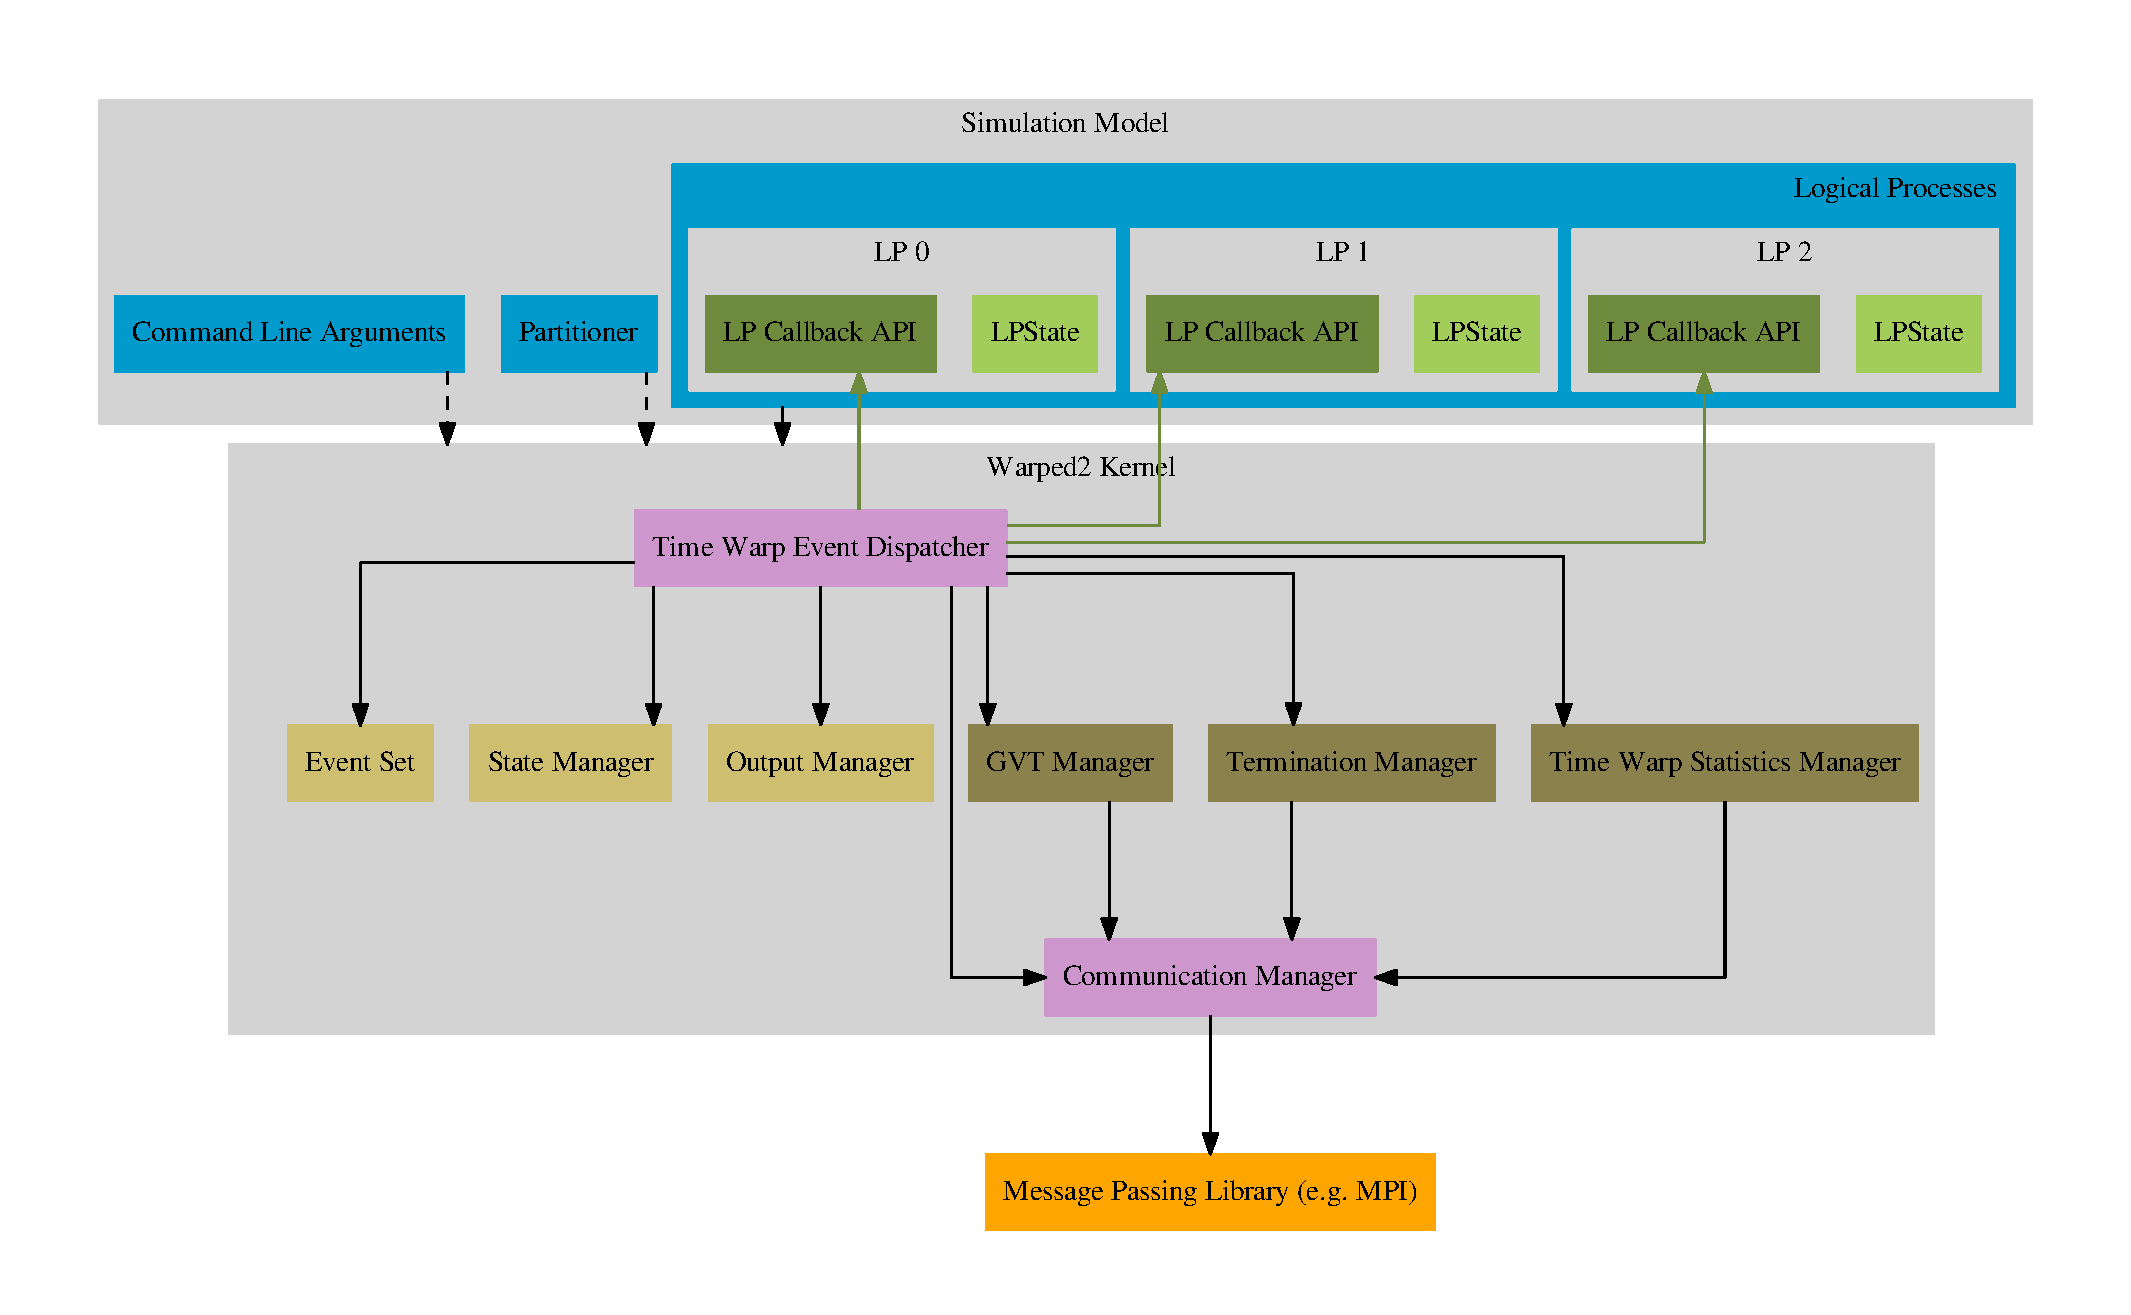
\includegraphics[width=\textwidth,quiet]{figs/graphviz/warped2_overview.pdf}
    \caption{Time Warp Components in \textsc{warped2}}\label{warped2_architecture}
\end{figure}

The Time Warp components can be categorized as either a local Time Warp component or a global Time
Warp component.  The local Time Warp components are used only for the local control mechanism of the
individual LPs such as rolling back and fossil collecting whereas the global Time Warp components
are concerned with the global control mechanisms such as GVT, termination detection and statistics
counting.  The global Time Warp components must be able to communicate with all other processes in
the system so that it is possible to determine the global state of the system.

\subsection{Local Time Warp Components}

The three local Time Warp components are \begin{inparaenum}[(1)] \item the EventSet,
\item the OutputManager, and \item the StateManager\end{inparaenum}.  The \texttt{OutputManager} and
  \texttt{StateManager} are abstract base classes that have a well defined API for cancellation and
  state saving techniques, respectively.

\paragraph{The EventSet} contains the data structures for all of the unprocessed and
processed events for the LPs that are local to the process.  This includes the input queues for each
LP and also the LTSF queues.  The event set provides methods for obtaining the next event,
processing a rollback, and fossil collecting processed events.  All the data structures that have
pending events must necessarily be thread safe since multiple worker threads could access them.

\paragraph{The OutputManager} contains all of the output queues and implements a single
cancellation technique.  The derived class must implement methods for adding an event to an output
queue, processing a rollback, and fossil collecting old output events.  Currently, \textsc{warped2}
only implements aggressive cancellation through the \texttt{AggressiveOutputManager} subclass but
may support more cancellation techniques in the future such as lazy cancellation.

\paragraph{The StateManager} contains all of the state queues and implements a single technique
for state saving and state restoration.  The derived class must implement methods for saving the
state of an LP, restoring the state of an LP, and fossil collecting old states.  Currently,
\textsc{warped2} only implements periodic state saving through the \texttt{PeriodicStateSaving}
subclass.

\subsection{Global Time Warp Components}

The three Time Warp components are \begin{inparaenum}[(1)] \item the GVTManager, \item the
  TerminationManager, and \item the StatisticsManager \end{inparaenum}.  The \texttt{GVTManager} is
an abstract base class which defines a well defined API for a GVT algorithm but the
\texttt{TerminationManager} and \texttt{StatisticsManager} are concrete classes which implement a
termination detection algorithm and a central statistics manager, respectively.

\paragraph{The GVTManager} keeps track of the GVT and implements a specific Global Virtual Time
(GVT) algorithm.  Due to the hybrid communication design of \textsc{warped2}, the GVT algorithms
will have some contribution from the worker threads and must also use the
\texttt{CommunicationManager} for a message passing algorithm to use between the set of processes.
Currently, \textsc{warped2} implements an \texttt{AsynchronousGVTManager} and a
\texttt{SynchronousGVTManager}.  The algorithms implemented within each one will be detailed further
in Chapter \ref{gvt_termination}.

\paragraph{The TerminationManager} implements an algorithm for determining when all processes
become inactive and initiates termination when that occurs.  In a manner similar to the
\texttt{GVTManager}, some contribution must come from the worker threads within each process and
each process must communicate through the \texttt{CommunicationManager}.  A more detailed
description of the termination detection algorithm used in \textsc{warped2} is given in Chapter
\ref{gvt_termination}.

\paragraph{The StatisticsManager} keeps track of all local statistics and provides methods for
performing global reductions on the them.  

\subsection{CommunicationManager}

The \texttt{CommunicationManager} provides an interface between the underlying message passing
library and the global time Warp components in the \textsc{warped2} simulation kernel.  Any
interprocess communication must go through the \texttt{CommunicationManager}, including remote
events that must be sent to another process or received from another process.  Any class that has to
do interprocess communication must register message types and a recieve callback function for each
type with the \texttt{CommunicationManager}.  More details on how to do this will be presented in
the next section. Currently, \textsc{warped2} only implements an MPI based
\texttt{CommunicationManager} through the \texttt{MPICommunicationManager} subclass.

\subsection{Partitioner}

The \texttt{Partitioner} is an abstract base class for implementing a method of logical process
partitioning.  Given a vector of LPs and some number of partitions, $N$, the partitioner object
returns $N$ vectors of LPs by using some partitioning technique.  The \textsc{warped2} kernel
implements a \texttt{RoundRobin} partitioner and a \texttt{ProfileGuidedPartitioner} but also allows
simulation models to define their own custom partitioners.  More details of these partitioning
techniques are given in Chapter \ref{partitioning_communication}.

\subsection{Implementation Details}

\subsubsection[Rollbacks \& Cancellation]{Data Structures to Support Rollbacks}

Jefferson \cite{jefferson-85} described the rollback and cancellation process in terms of three data
structures: the input queue, output queue, and state queue.  The data structures that are
implemented in \textsc{warped2} follows closely to Jefferson's description except that in
Jefferson's approach, the input queue holds both unprocessed and processed events whereas
\textsc{warped2} has two separate data structures to allow easier scheduling of unprocessed events.

The state queues contain a 3-tuple value for each state.  The first value is a pointer to a memory
location which holds the saved copy of the LP state.  The second value is a pointer to the event
that produced the state of the LP and is used for comparison against a straggler event on a rollback
to determine which state to restore or against the GVT during fossil collection.  The third value is
the state of the LPs random number generators at the time the state was saved.  The random number
generator states are saved in a linked list and are also restored during a rollback to ensure
deterministic results.

Similar to the state queue, the output queue also contains a tuple of values.  In the output queue
though, only a pointer to a source event and a sent event are used.  In the same way as the state
queue, the source event is used for comparison against a straggler event during a rollback but is
used to determine which sent events should be sent as anti-messages.

The processed queues only contain a pointer to the processed events.  The events referred to by all
data structures all share the same memory so that memory is conserved and copying is avoided.
Furthermore, if events are sent within the same process, the same events can be referred to from the
output queue and an unprocessed or processed event from another LP.  The organization of the
processed queue, state queue and output queue for a single LP is illustrated in Figure
\ref{rollback_ds}.

\begin{figure}
    \centering
    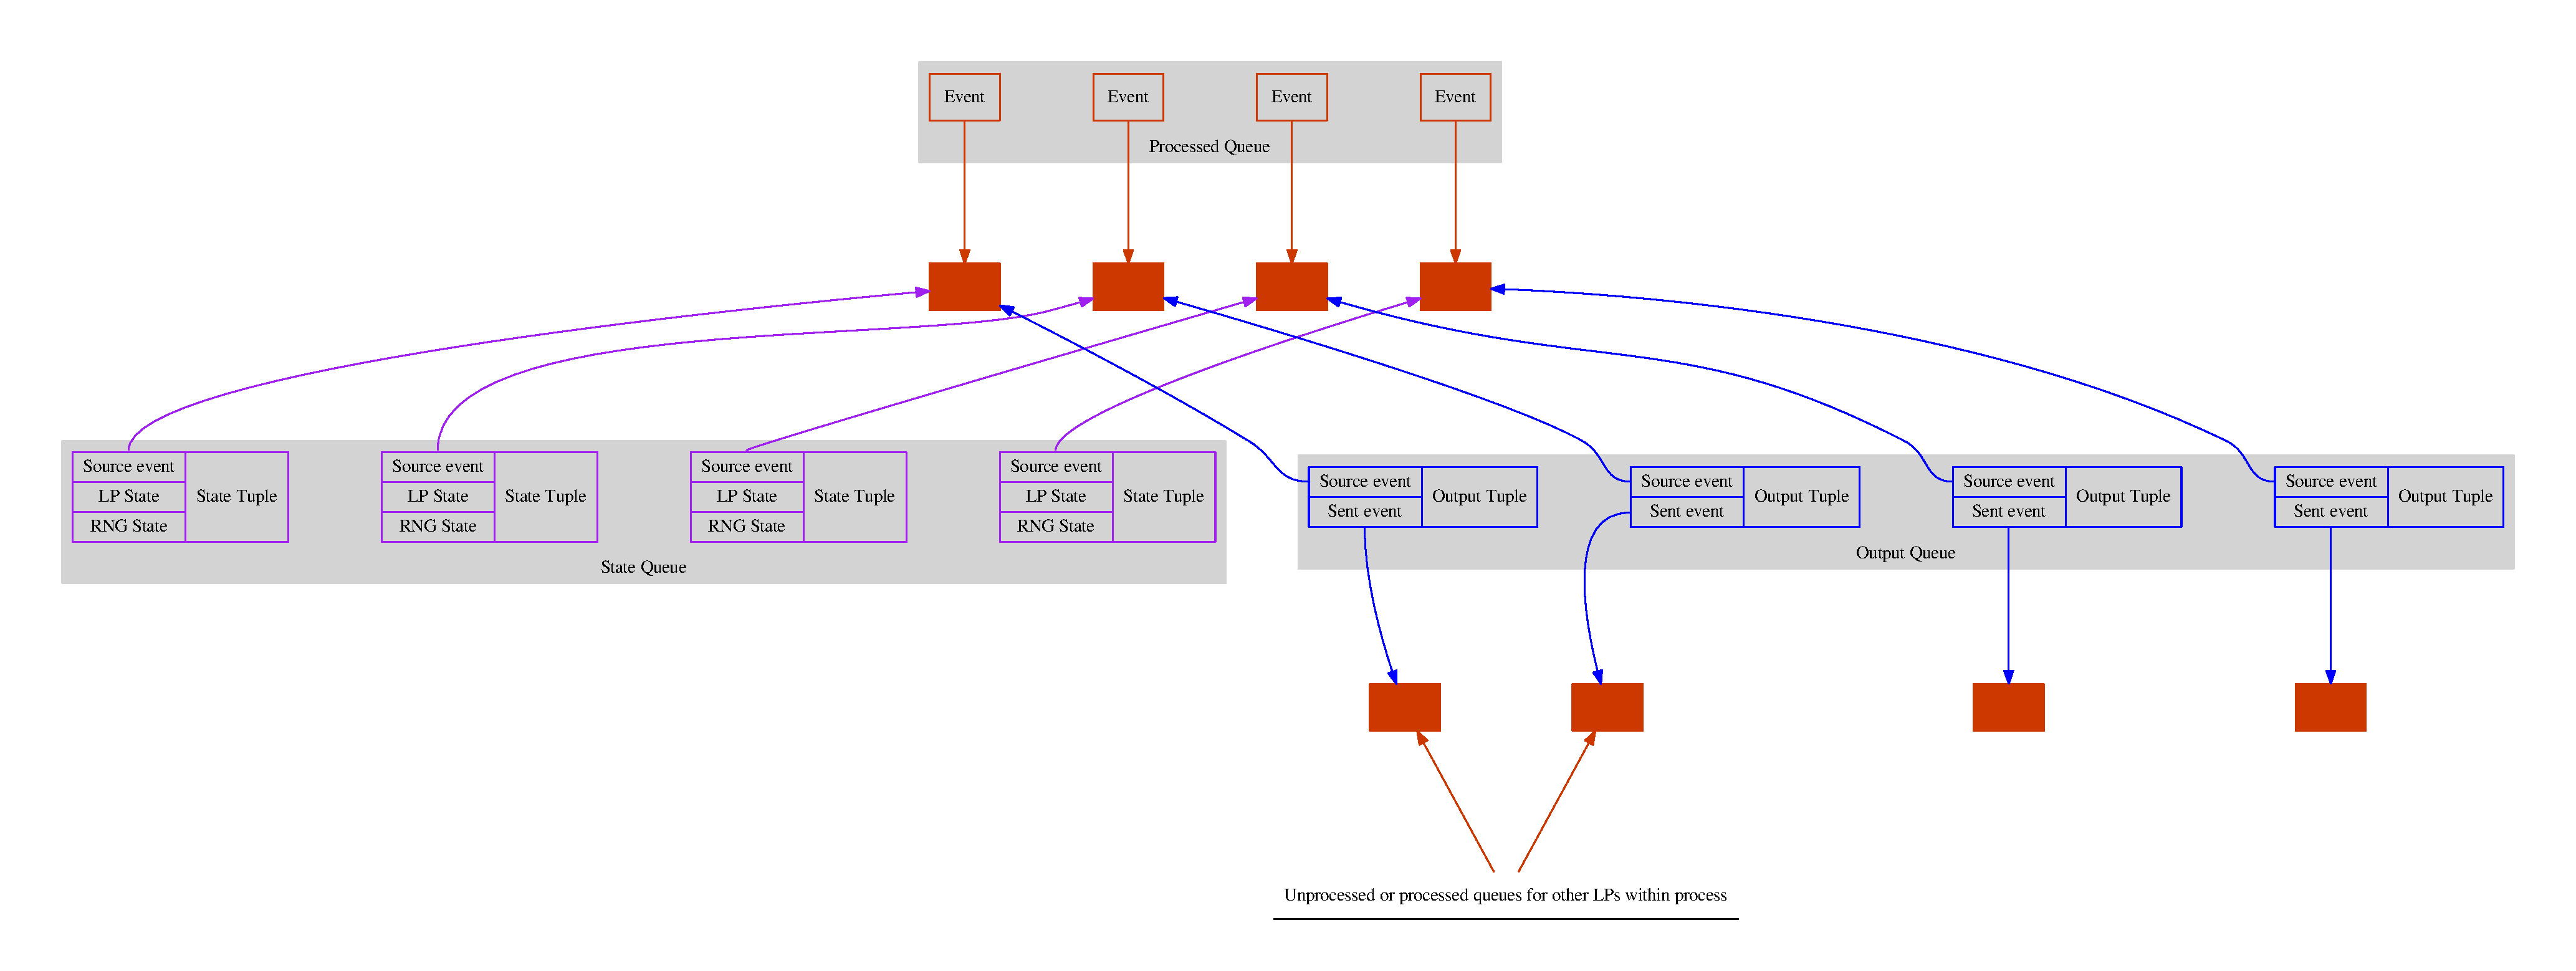
\includegraphics[width=\textwidth,quiet]{figs/graphviz/rollback_ds.pdf}
    \caption{Rollback and Cancellation Data Structures in \textsc{warped2}}\label{rollback_ds}
\end{figure}

Although the organization of these data structures prevents copying of events or timestamp
information, there are also some limitations.  First, it introduces a significant amount of indirect
memory accesses which could slow down access to memory, especially in a multiprocessor system.
Secondly, it adds some complexity when events must be fossil collected.  To solve this problem
though, \textsc{warped2} uses the smart pointers offered by the standard C++11 libraries which
maintain a reference count and automatically free memory when the reference count reaches zero.

\subsubsection{Message Passing Communication and Serialization}

For any Time Warp component that must use the message passing library must register a message type
with the communication manager.  When the message type is registered, a receive callback method that
is linked to the message type is also registered so that any messages received with that type can be
handled appropriately.

To create a message type, the name of the type must first be added to the \texttt{MessageType} enum
as a new value.  Then the new type must then be defined by deriving from the
\texttt{TimeWarpKernelMessage} base class.

The receive callback is defined in the class that sends the message just as any other class method.
The callback method must have a \texttt{void} return type and take a single argument of type
\texttt{std::unique\_ptr<TimeWarpKernelMessage>}.  For simplicity, the
\texttt{WARPED\_REGISTER\_MSG\_HANDLER} macro can be used to register the message types and receive
callback as long as the communicating class contains a data member that is declared exactly as
\texttt{std::shared\_ptr<CommunicationManager> comm\_manager\_;}.

The message types must all be serializable which means that all member variables within the message
type define must be registered with the serialization API so that a storage order can be defined.
To do this, the \texttt{WARPED\_REGISTER\_SERIALIZABLE\_MEMBERS} macro is provided.  All member
variable must be passed to this macro as well as
\texttt{cereal::base\_class<TimeWarpKernelMessage>(this)} to ensure that all base class members are
also serialized.  The order that the members are listed is completely arbitrary.  In addition, the
message type must be registered using the
\texttt{WARPED\_REGISTER\_POLYMORPHIC\_SERIALIZABLE\_CLASS} macro.



\chapter{Plans of Study}\label{plans_of_study}

Experimental results will be presented throughout the remaining chapters as the various aspects
of \textsc{warped2} are discussed.  All chapters will contain experimental results for (i) a single
x86 SMP nodes and (ii) a cluster of x86 SMP nodes.   The chapters will evaluate the performance on
each platform with a goal of understanding and determining the best design options and
configurations for generalized use in either framework.

The single node SMP experiments will be run on an Intel\textsuperscript{\textregistered}
Xeon\textsuperscript{\textregistered} X5675 processor.  The Intel\textsuperscript{\textregistered}
Xeon\textsuperscript{\textregistered} X5675 has 6 cores with hyperthreading so that 12 simultaneous
threads can be executed.  Cluster experiments will be run on Intel\textsuperscript{\textregistered}
Xeon\textsuperscript{\textregistered} E5410.  The Intel\textsuperscript{\textregistered}
Xeon\textsuperscript{\textregistered} E5410 is a quad core processor but each machine contains two
sockets so that two processors can be used which gives a total of 8 cores per machine.  A summary of
the architectural features and runtime software for both machines are summarized in table
\ref{x86_platform} found in appendix \ref{x86_nodes_and_clusters}.

Throughout the rest of this text, a number of different measures will be used for comparison of
different optimizations and configurations.  The \emph{efficiency} and \emph{event rate} are two
examples of measures that are used the most so they are introduced here.  Other measures will be
introduced as needed.  The efficiency is defined as:

$$ Efficiency = {events_{committed}}/{events_{processed}} * 100 $$

\noindent
where $events_{committed}$ is the number of events that are processed and not rolled back and
$events_{processed}$ is the total number of events that are processed whether they are rolled back
or not.  Thus, the efficiency is a measure of the percentage of events that are processed and not
rolled back.  The event rate is defined as:

$$ Event Rate = {events_{committed}}/{runtime} $$

\noindent
where $runtime$ is the real time that it takes for the simulation the complete and
$events_{committed}$ is again the total number of events processed and not rolled back.

\section{Experiments}

The experiments carried out on a single node SMP machine will be strongly tied to thread
synchronization, state saving, memory allocation, and fossil collection.  On the other hand,
experiments carried out on a cluster will be strongly tied to communication, partitioning, state
saving, and scaling up simulations.  The experiments for a single SMP node are summarized in table
\ref{smp_experiments} and for a cluster in table \ref{cluster_experiments}.

\begin{table}[H]
    \centering
    \begin{tabular}{| c | c | c | c |}
        \hline
        \textbf{Comparison} & \textbf{Measure(s)}  & \textbf{Figure(s)}   & \textbf{Machine(s)}  \\
        \hline
        Number of LTSF Queues & Event Rate and Efficiency   & Figure \ref{ltsf_analysis}    & X5675             \\
        \hline
        LTSF Queue Partitioning & Time and Efficiency    & Figures \ref{ltsf_partitioning_bc},
            \ref{ltsf_partitioning_beowulf}    & X5675, E5410 \\
        \hline
        State Saving Period & Event Rate, ...  & Figure \ref{ssp_analysis_smp_performance} & X5675 \\
        \hline
        Spinlocks & Speedup  & Figure \ref{spinlock_speedup} & X5675 \\
        \hline
        Fossil Collection Techniques & Event Rate    & Figure \ref{fc_times} & X5675 \\
        \hline
        Memory Allocators & Event Rate   & Figure \ref{allocator_analysis_eventrate} & X5675 \\
        \hline
        Memory Allocators & Efficiency   & Figure \ref{allocator_analysis_efficiency}    & X5675 \\
        \hline
        LTSF Queues & \% Memory Increase & Figure \ref{ltsf_memory}  & X5675 \\
        \hline
        State Saving Period & \% Memory Decrease & Figure \ref{ssp_analysis_smp_memory}  & X5675 \\
        \hline
        GVT Period & Memory and Time & Figure \ref{fc_memory_analysis}   & X5675 \\
        \hline
    \end{tabular}
    \caption{SMP Node Experiments}\label{smp_experiments}
\end{table}

\begin{table}[H]
    \centering
    \begin{tabular}{| c | c | c | c |}
        \hline
        \textbf{Comparison} & \textbf{Measure(s)}  & \textbf{Figure(s)}   & \textbf{Machine(s)}  \\
        \hline
        Communication Model & Event Rate & Figure \ref{communication_model_eventrate}  & E5410 \\
        \hline
        Communication Model & Efficicency & Figure \ref{communication_model_efficiency}  & E5410 \\
        \hline
        Interprocess Partitioning & Event Rate, Efficiency, \% Remote Events   & Figure \ref{partitioning_8node} & E5410 \\
        \hline
        Aggregate Messages & Event Rate & Figures \ref{aggregate_eventrate} & E5410 \\ 
        \hline
        Aggregate Messages & Efficiency & Figures \ref{aggregate_efficiency} & E5410 \\ 
        \hline
        Aggregate Messages & Average Rollback Length & Figures \ref{aggregate_rblength} & E5410 \\ 
        \hline
        Scaling LPs & Efficiency, \% Remote Events, Event Rate & Figure \ref{scaling}    & E5410 \\
        \hline
        State Saving Period & Event Rate, ... & Figure \ref{ssp_analysis_cluster} & E5410 \\
        \hline
        State Saving Period & \% Memory Decrease & Figure \ref{ssp_analysis_smp_memory}  & E5410 \\
        \hline
    \end{tabular}
    \caption{Cluster Experiments}\label{cluster_experiments}
\end{table}

\section{Simulation Models}

This section describes some of the \textsc{warped2} simulation models that will be used for
experiments.  Most of these models are similar to and inspired by simulation models studied and
reported upon by other parallel simulation researchers.  The model configurations that are used are
included within tables in Appendix \ref{model_configurations}.

\subsection{PCS}

The model describes a type of wireless communication network known as a \emph{Portable Cellular
  Service (PCS)} network.  A PCS network provides services for a number of \emph{portables} that are
the subscribers to the network.  The service area of the network is divided into \emph{cells} and a
single \emph{port} covers a single cell which has a certain number channels that it can allocate for
calls.  When an incoming or outgoing call is made, a port must allocate a channel from the port and
if one cannot be allocated then the call is \emph{blocked}\cite{lin-96b}.  The only type of logical
processes in the PCS simulation are the cells.  The cells in the \textsc{warped2} model form a
rectangular grid as shown in Figure \ref{pcs_model_lps}.  Portables can only move to other cells
from an adjacent cell with a wrap around occurring at the edges.

\begin{figure}
    \centering
    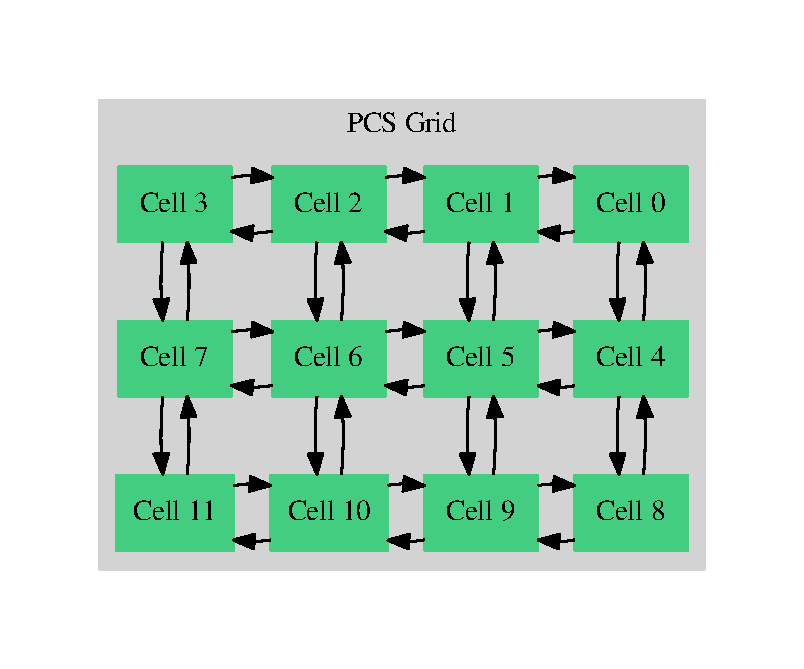
\includegraphics[width=0.6\textwidth,quiet]{figs/graphviz/pcs_model.pdf}
    \caption{PCS Model Logical Processes}\label{pcs_model_lps}
\end{figure}

The portables stay within a cell for a period of time which follows a Poisson distribution
before moving to another cell.  If the all cells are busy in the cell that the portable
is moving to then the call is dropped.  This is called a \emph{handoff block}.

Every LP keeps track of the following state variables:
\begin{itemize}
    \item Number of idle channels
    \item Number of call attempts
    \item Number of channel blocks
    \item Number of handoff blocks
\end{itemize}

\noindent
Call arrivals to a portable also follow a Poisson distribution.  The cells in the model generate all
of their own incoming calls in a self-initiating process.  Four types of events are used to model
the network: \begin{inparaenum}[(1)] \item \texttt{NextCall},
\item \texttt{CallCompletion}, \item \texttt{PortableMoveOut}, and \item \texttt{PortableMoveIn}
\end{inparaenum}.  The \texttt{NextCall}, \texttt{CallCompletion}, and \texttt{PortableMoveOut}
events are all sent to self whereas the \texttt{PortableMoveIn} event is sent to an adjacent
cell based on a random variable with uniform probability.

\subsection{Traffic}

The traffic simulation model is derived from a similar simulation model found in the ROSS
\cite{carothers-00} code base.  The traffic model describes a grid of intersections and the movement
of cars through the intersections and between the intersections.  All intersections are four way
intersections and have three lanes in each direction.  The LPs in the traffic model are the
intersections and form a rectangular grid in the same way as that of the PCS model.

The simulation starts with a uniform distribution of cars at each intersection and each car is a
assigned a destination which it finishes at.  With each arrival at an intersection the car always
first tries to go in the direction that gets it closer to its destination.  The number of cars going
out of an intersection in the same direction is limited to a maximum number due to traffic on the
destination road.  An incoming car that cannot travel in a specific direction because of traffic is
forced to wait or take another route.  For each intersection, the state consists of:

\begin{itemize}
    \item Number of cars coming into the intersection from each direction
    \item Number of cars going out of the intersection to each direction
    \item Total cars arrived at the intersection
    \item Total cars finished at the intersection
\end{itemize}

A car goes through three event phase in every intersection as shown in Figure
\ref{traffic_events}.  The three types of events are: \begin{inparaenum}[(1)] \item Arrival,
\item Direction Select, and \item Departure \end{inparaenum}.  The arrival and departure events are
mainly used for simple state updates and timing of the next events.  The direction select event is
where the complexity of the simulation is and determines the direction that the car should go in
order to reach its destination or whether the car should take another route due to traffic.

\begin{figure}
    \centering
    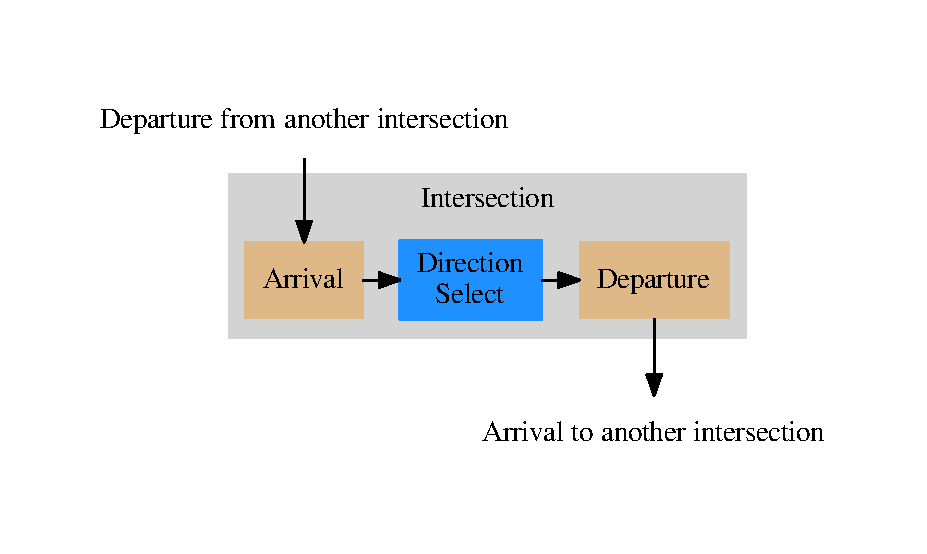
\includegraphics[width=0.6\textwidth,quiet]{figs/graphviz/traffic_events.pdf}
    \caption{Intersection Event Sequence}\label{traffic_events}
\end{figure}

All events in the traffic model follow an exponential distribution and a single event is generated
with the processing of each event.  The departure and direction select events are self-generated but
the arrival event are received from an adjacent intersection.

\subsection{Epidemic}

The epidemic model describes the spreading of an infectious disease across a set of geographic
locations in a region and across a set of regions.  The logical processes in the simulation are
geographic locations which represent a portion of the population.  The interactions between people
in different geographic locations and regions are modeled with a diffusion network.  An abstract
view of the simulation model is shown below in Figure \ref{epidemic_model}.

\begin{figure}
    \centering
    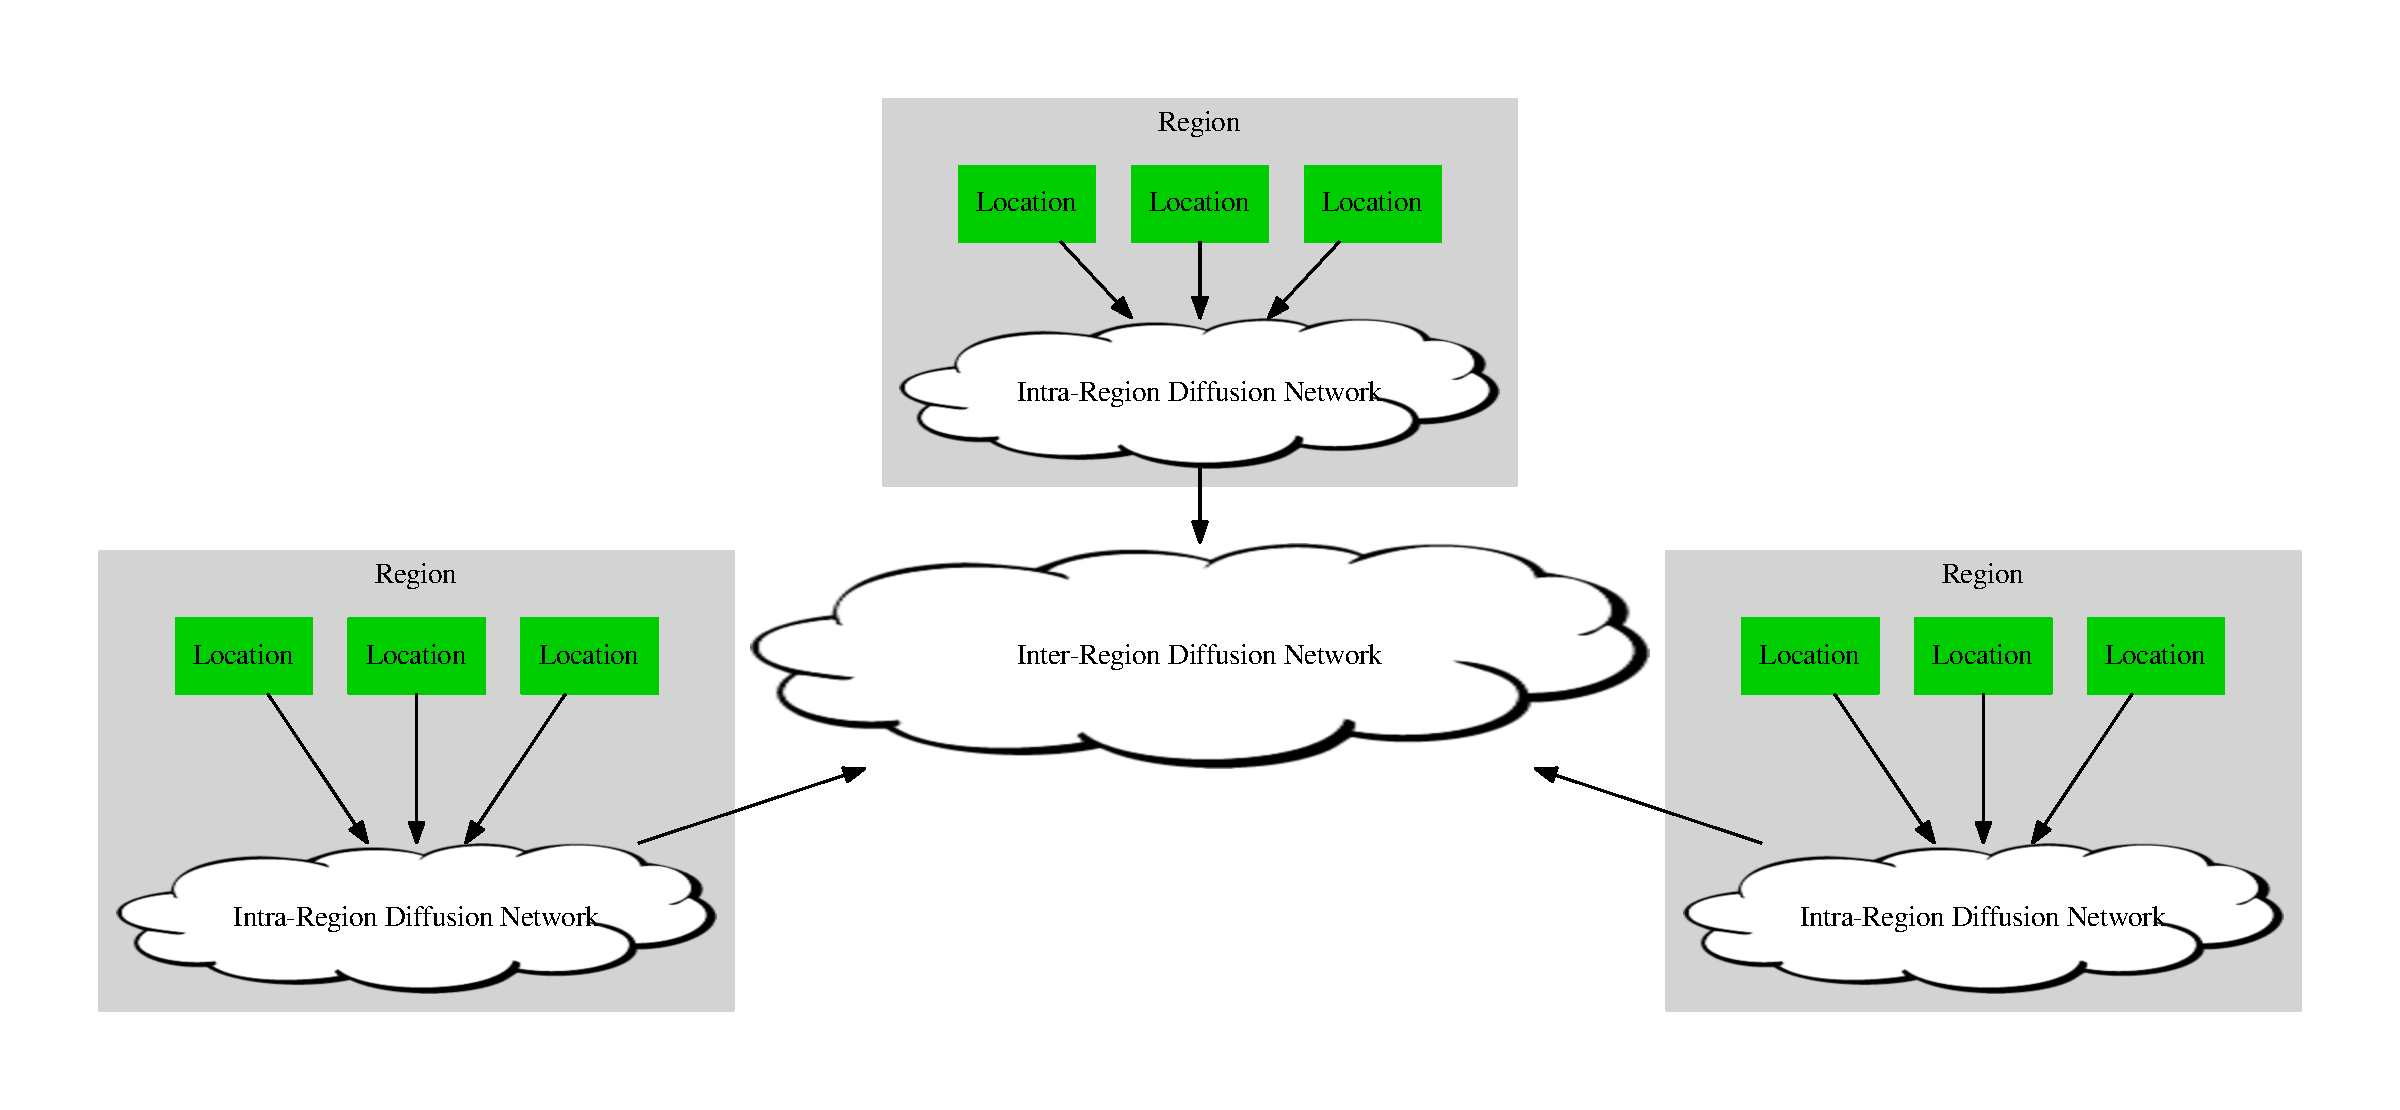
\includegraphics[width=0.6\textwidth,quiet]{figs/graphviz/epidemic.pdf}
    \caption{Epidemic Model}\label{epidemic_model}
\end{figure}

The model is based on reaction-diffusion model \cite{perumalla-12}.  A reaction process models the
behavior of the disease within a person as well as the transmission of the disease between people
within the same location.  A probabilistic reaction function defines the behavior of the disease
between individuals \cite{barrett-08}.  The disease within an individual is modeled by a
Probabilistic Timed Transition System (PTTS) \cite{barrett-08} which is a finite state machine
describing states of the disease and the transitions between states.  Together, the reaction
function and PTTS models of the disease form the \emph{disease model}.  The diffusion network models
the social interactions of people between locations and between regions \cite{barrett-08}.

\subsection{Airport}

The airport model describes the departure and arrivals of airplanes between a connected set of
airports.  The logical processes represent airports and the events are simply departures and
arrivals.  For simplicity, the airports are connected in a rectangular grid and can only fly to
airports to the north, east, south, or west of the airport departed from.  The time spent between
takeoff and landing and between landing and takeoff both follow an exponential distributions.



\chapter[Communication]{Interprocess Communication} \label{partitioning_communication}

One of the main goals of \textsc{warped2} is to efficiently use shared data structures among a set
of worker threads executing on the same node while also allowing remote communication among multiple
processes executing on multiple nodes.  To achieve this, a message passing system must be setup so
that all threads of a single process can send events to LPs handled by remote processes.  This first
part of this chapter describes an overview of different communication models that have been
considered in the design and implementation of \textsc{warped2}.  Then some techniques to minimize
remote communication such as partitioning and message aggregation are discussed and various
configurations for each are compared.

\section{Multithreaded Message Passing with MPI}

Message passing between processes in \textsc{warped2} is currently implemented with MPI.  The MPI
standard says that an MPI implementation may support up to four different levels of thread support
for an application:

\begin{description}
    \item[MPI\_THREAD\_SINGLE:] The application uses only a single thread.
    \item[MPI\_THREAD\_FUNNELED:] The application is multithreaded but only a single thread will
      make MPI calls.
    \item[MPI\_THREAD\_SERIALIZED:] The application is multithreaded but only a single thread at a
      time will make MPI calls.
    \item[MPI\_THREAD\_MULTIPLE:] The application is multithreaded and threads have no restrictions.
\end{description}

For the remainder of this discussion, the thread models listed above will be referred to as simply
single, funneled, serialized, and multiple.  The funneled communication model can increase latency
because the thread that handles communication may be busy doing some other work so an extra step
will be necessary to temporarily queue remote events to be sent.  Furthermore, if communication is
too fine-grained, then some type of flow control may also be necessary.  Serialized or full multiple
thread communication, on the other hand, can increase contention for access to MPI library calls and
slow down the worker threads.  It will also force worker threads to take more time for
serialization, deserialization, and memory allocation/deallocation.  The singled threaded
communication model does not really fit the needs of \textsc{warped2} but is mentioned for
completeness.

The plots in Figures \ref{communication_model_eventrate} and \ref{communication_model_efficiency}
compare the event rates and efficiencies for all of the communication models with the Epidemic, PCS,
and Traffic models.  For serialized communication, a single global spinlock is used to serialize
access to all MPI library calls.  For funneled, serialized, and multiple threaded communication
models, 7 worker threads and a manager thread are used per node and for single threaded
communication, 8 processes per node are used with no manager thread.

\begin{figure}
  \begin{minipage}{.5\textwidth}
    \begin{center}
      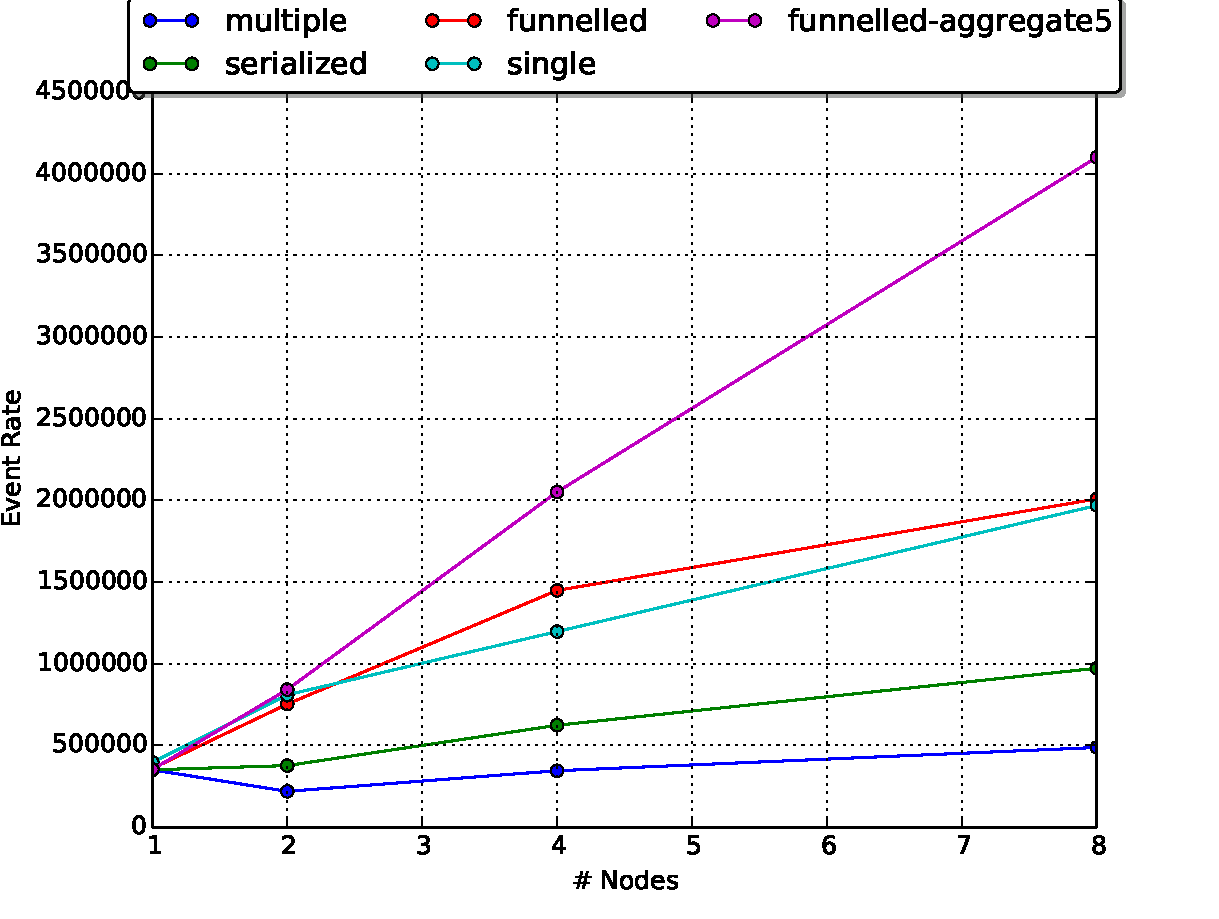
\includegraphics[width=\textwidth,keepaspectratio,quiet]{figs/partitioning_communication/communication_pcs_eventrate.pdf} \\
      PCS \\
    \end{center}
  \end{minipage}%
  \begin{minipage}{.5\textwidth}
    \begin{center}
      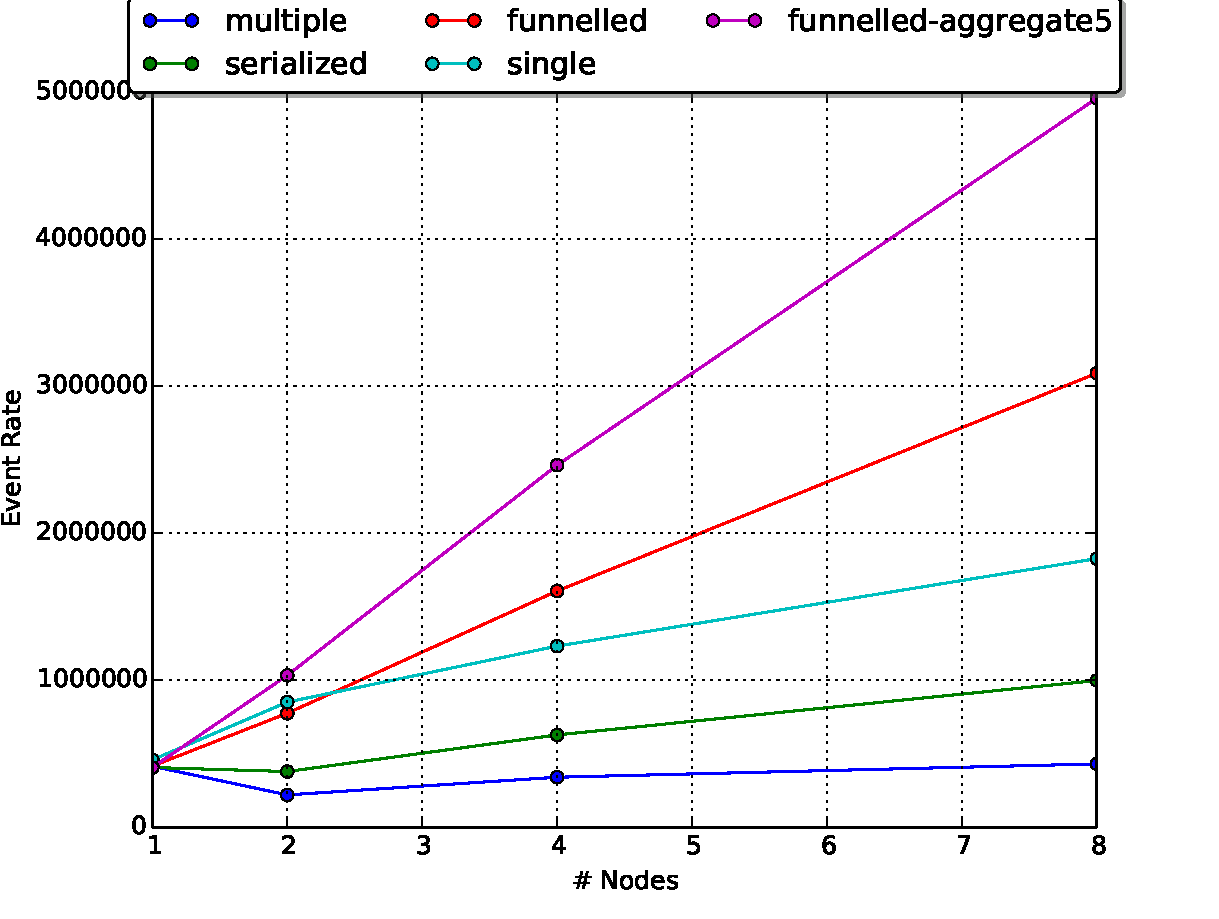
\includegraphics[width=\textwidth,keepaspectratio,quiet]{figs/partitioning_communication/communication_traffic_eventrate.pdf} \\
      Traffic \\
    \end{center}
  \end{minipage}
  \centering
  \begin{minipage}{.5\textwidth}
    \begin{center}
      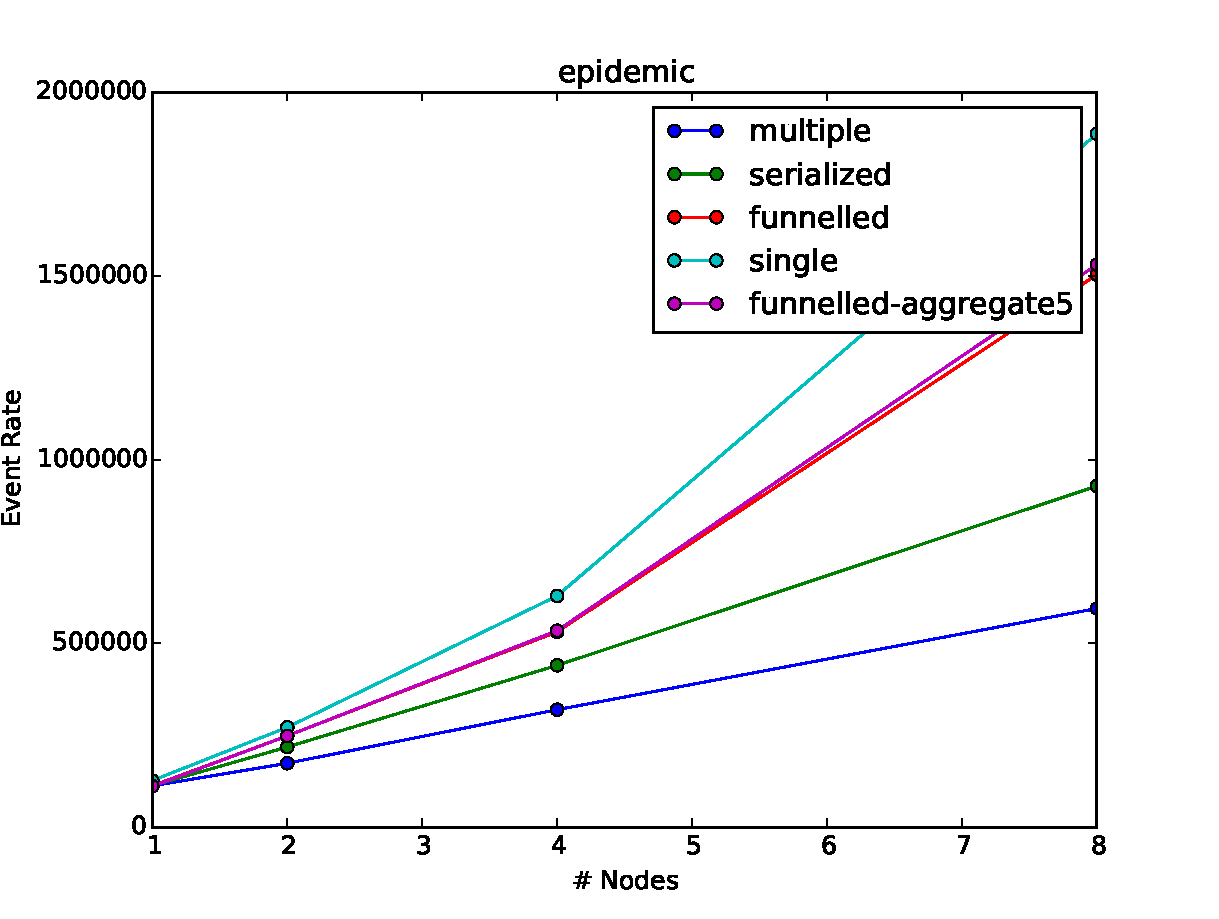
\includegraphics[width=\textwidth,keepaspectratio,quiet]{figs/partitioning_communication/communication_epidemic_eventrate.pdf} \\
      Epidemic \\
    \end{center}
  \end{minipage}
  \caption{Communication Models: Event Rate}\label{communication_model_eventrate}
\end{figure}

The single threaded and funnelled communication models show much better performance than a
serialized or multiple threaded communication model.  This indicates that lock contention is
inhibits performance more than an extra remote communication or an increase in latency due to a
queueing delay.  However, as shown in Figure \ref{communication_model_efficiency}, the efficiency
decreases at a pretty fast rate as the number of nodes increase for singled threaded and funnelled
communication which could lead to less performance gain as the number of nodes is scaled up.

\begin{figure}
  \begin{minipage}{.5\textwidth}
    \begin{center}
      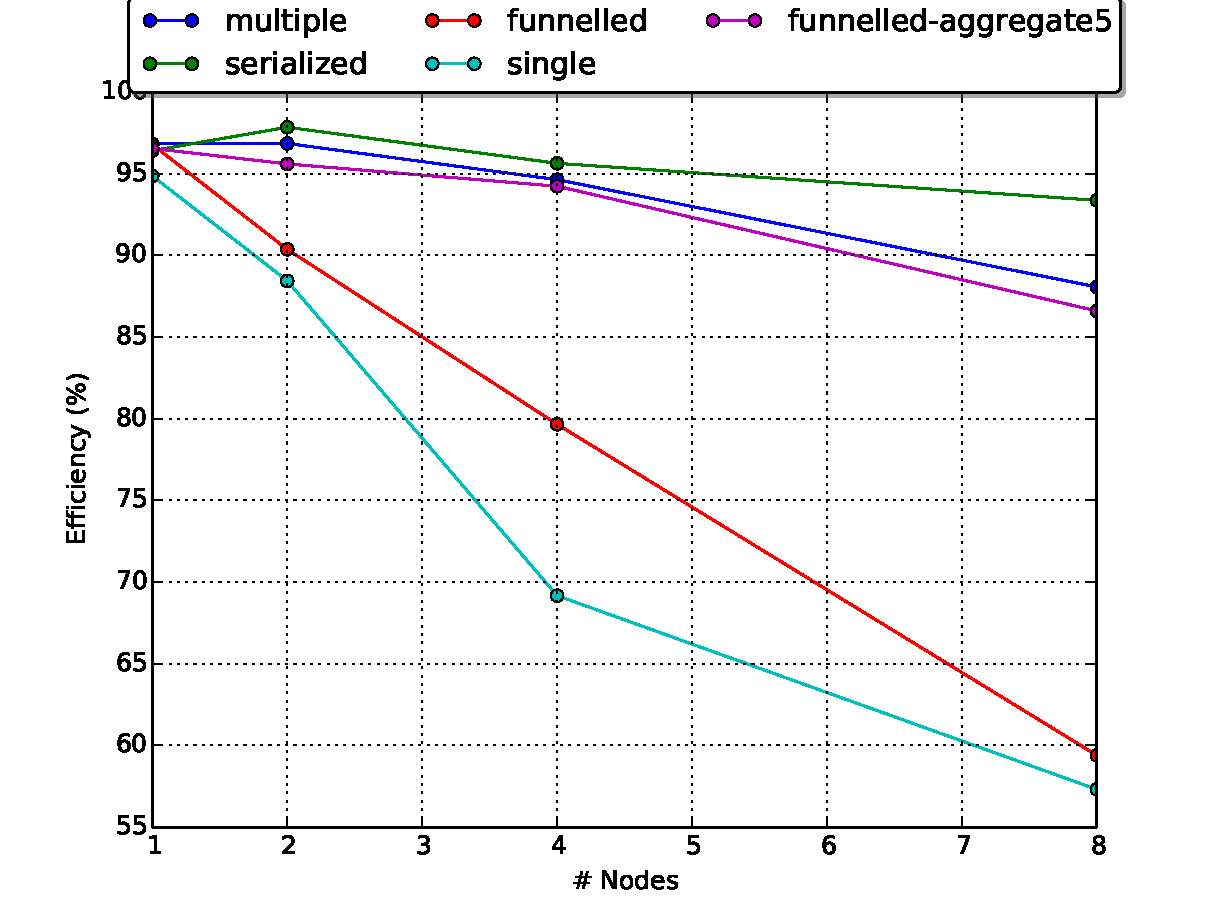
\includegraphics[width=\textwidth,keepaspectratio,quiet]{figs/partitioning_communication/communication_pcs_efficiency.pdf} \\
      PCS \\
    \end{center}
  \end{minipage}%
  \hfill
  \begin{minipage}{.5\textwidth}
    \begin{center}
      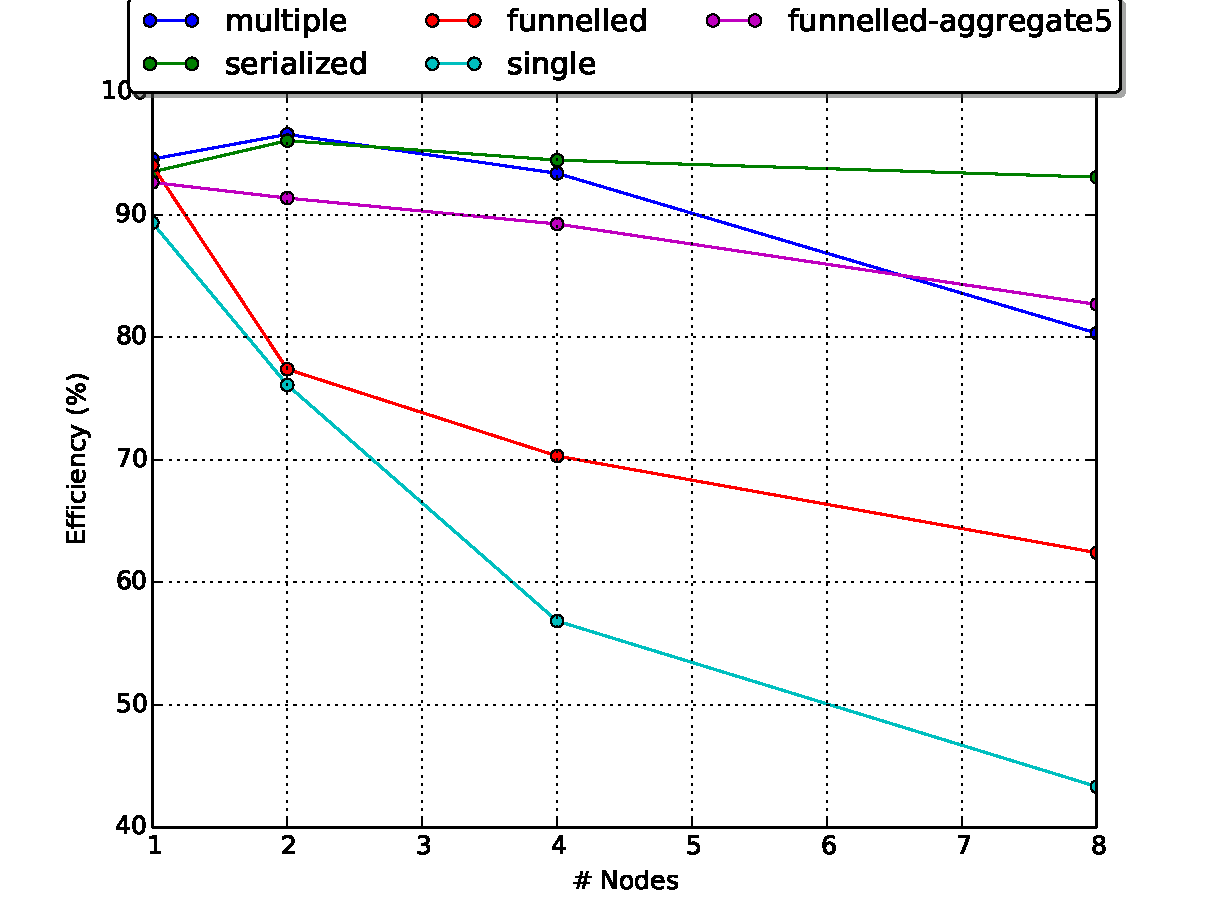
\includegraphics[width=\textwidth,keepaspectratio,quiet]{figs/partitioning_communication/communication_traffic_efficiency.pdf} \\
      Traffic \\
    \end{center}
  \end{minipage}
  \centering
  \begin{minipage}{.5\textwidth}
    \begin{center}
      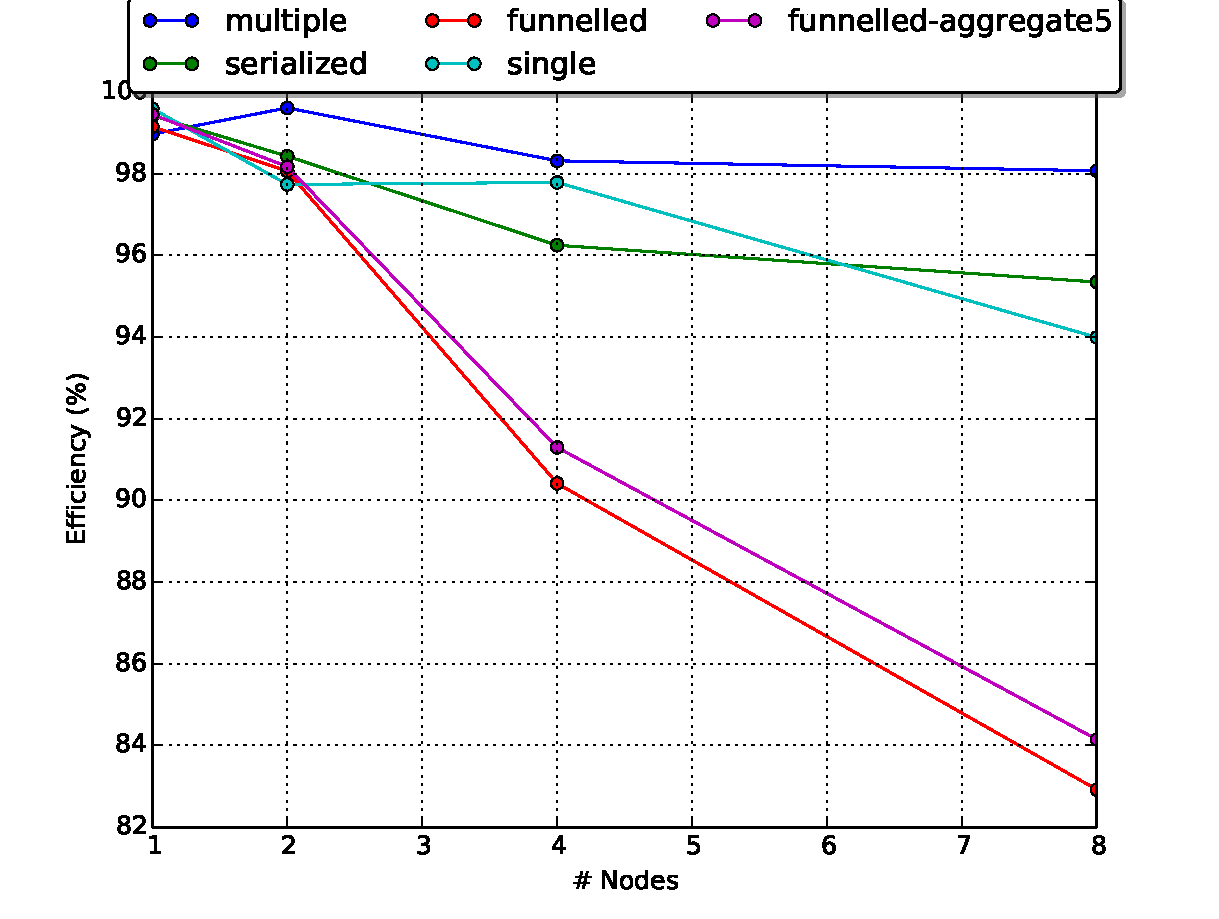
\includegraphics[width=\textwidth,keepaspectratio,quiet]{figs/partitioning_communication/communication_epidemic_efficiency.pdf} \\
      Epidemic \\
    \end{center}
  \end{minipage}
  \caption{Communication Models: Efficiency}\label{communication_model_efficiency}
\end{figure}

The efficiency can be improved with other methods that can be tuned in \textsc{warped2} such as
partitioning and message aggregation so it is not considered to be much of problem.  The rest of
this chapter will describe how this can be achieved in \textsc{warped2} by using parameters that can
be tuned based on the needs of specific simulation models.

\section{Communication Tuning Parameters}

To effectively scale simulations to larger number of nodes in a cluster, the interprocess
communication should be minimized as much as possible to avoid excessive communication which will
lead to more rollbacks.  To allow different types of models to run on larger scale cluster,
\textsc{warped2} allows the user to choose how to partition LPs among the MPI processes and how many
messages to aggregate for each receiver process.  The next two sections will provide any overview of
supported partitioning schemes and message aggregation in \textsc{warped2}.

\subsection{Interprocess Partitioning}

Partitioning the LPs among processes is necessary so that LPs that communicate with each other a lot
remain on the same node and minimize network communication in clusters.  When network communication
is minimized, the latency of sending events is decreased and will help to keep the number of
rollbacks down.  Currently, \textsc{warped2} supports three partitioning schemes:
\begin{inparaenum}[(1)] \item Round-Robin, \item Profile-Guided, and \item Custom \end{inparaenum}.  

\paragraph{Round-Robin} partitioning is a simple partitioning scheme where $blocksize$ number
of LPs are allocated to each process at a time and in order of increasing process id.  $blocksize$
can be between 1 and $NumLPs$/$NumProcesses$ where the latter is simply known as block partitioning.
From now on, a $blocksize$ of 1 will also be called simply round-robin.  A block size in between the
extreme values can be used in some models to make a second level partitioning scheme easier.  Figure
\ref{round_robin_partitioning} illustrates how a round-robin partitioning scheme would work with
different values for $blocksize$, where different partitions are represented by different colors and
the numbers represent an LP id.

\begin{figure}
  \begin{center}
    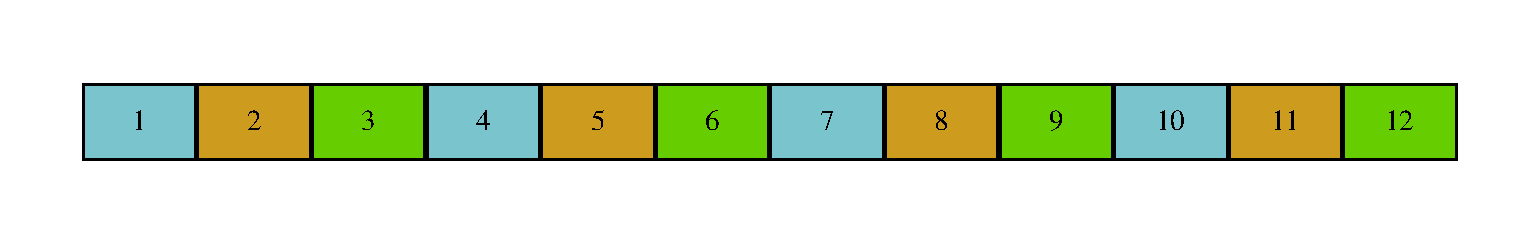
\includegraphics[width=0.8\textwidth,keepaspectratio,quiet]{figs/graphviz/round_robin_partitioning.pdf} \\
    Round-Robin with blocksize = 1 \\
    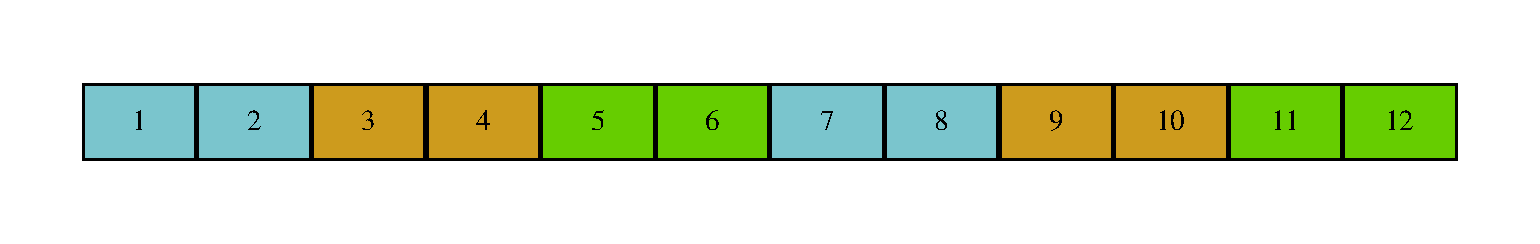
\includegraphics[width=0.8\textwidth,keepaspectratio,quiet]{figs/graphviz/block_rr_partitioning.pdf} \\
    Round-Robin with blocksize = 2 \\
    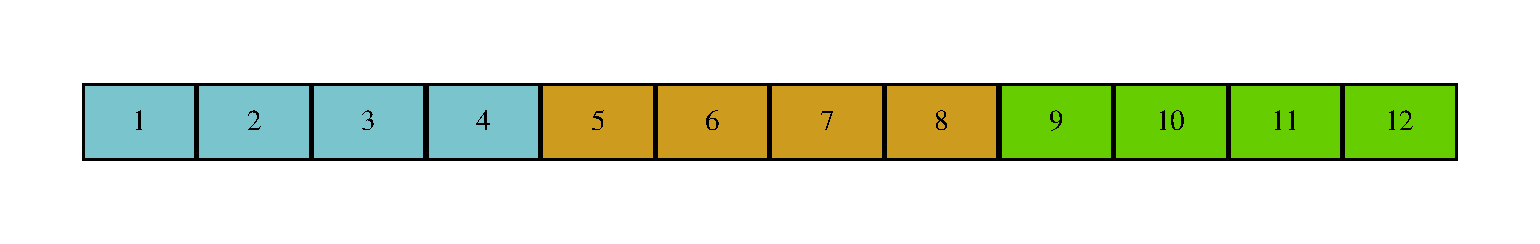
\includegraphics[width=0.8\textwidth,keepaspectratio,quiet]{figs/graphviz/block_partitioning.pdf} \\
    Round-Robin with blocksize = $NumLPs$/$NumProcesses$ (Block) \\
  \end{center}
  \caption{Round Robin Partitioning}\label{round_robin_partitioning}
\end{figure}

\paragraph{Profile-Guided} partitioning is based on profile data that is collected with a
sequential simulation.  The profile data contains a count of events for each communicating pair of
LPs.  When a Time Warp simulation is run, the partitioner uses that data to build a weighted graph
and uses a graph partitioning tool to create partitions that minimize the cut-set so that
cross-partition communication is minimized.  Profile-Guided partitioning should be used if a
simulation model has a peculiar communication pattern among LPs that is not suitable for round-robin
and does not implement a custom partitioning scheme.  It will also work well for any odd number MPI
processes which may not work well with other partitioning schemes.

The plots in Figure \ref{partitioning_8node} show a comparison of the round-robin, block, and
profile-guided partitioning schemes.  The data was collected with the full multithreaded
communication model where worker threads handle all remote communication.  For this reason, the
event rates and efficiencies will be significantly different than the mainline version of
\textsc{warped2} but should still be valid for the comparison of partitioning methods.

\begin{figure}
  \begin{minipage}{.5\textwidth}
    \begin{center}
      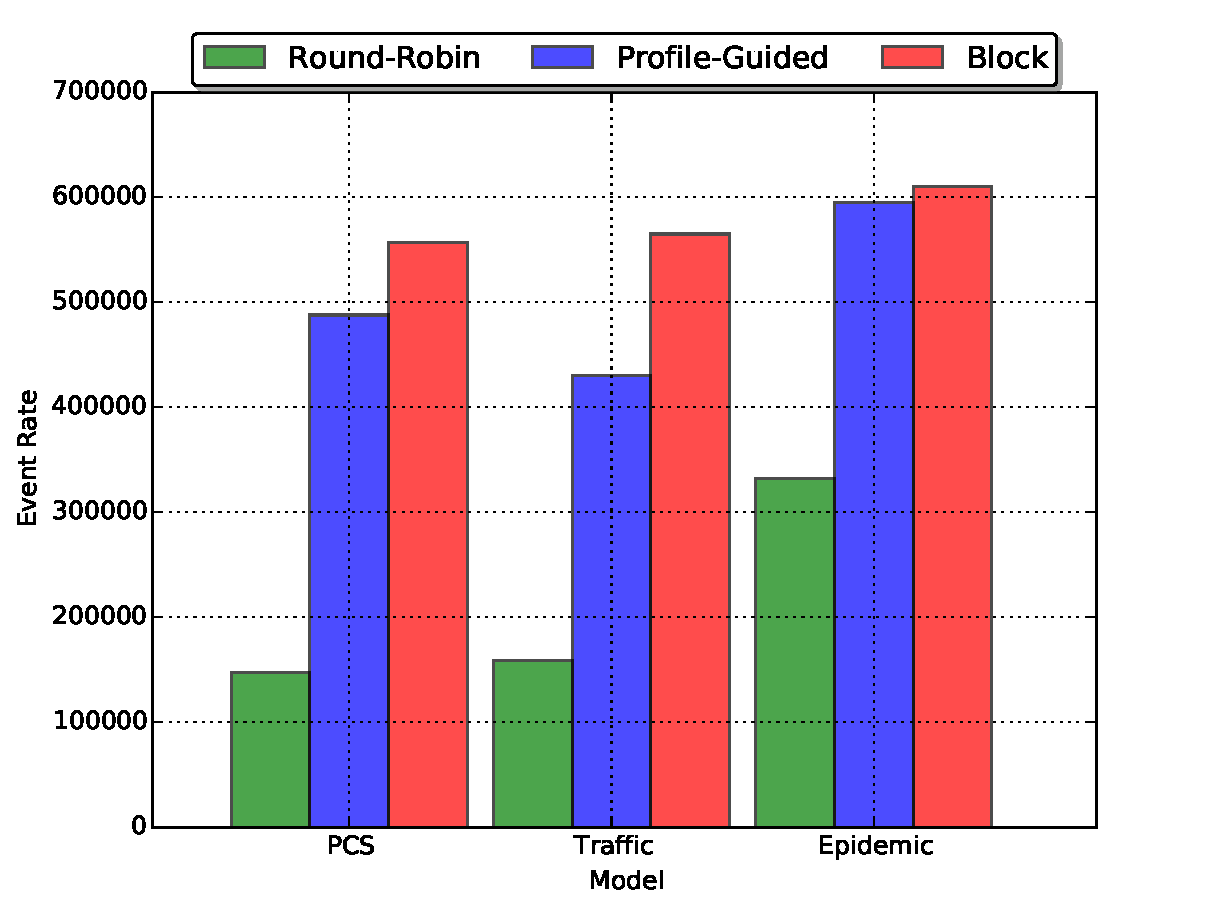
\includegraphics[width=\textwidth,keepaspectratio,quiet]{figs/partitioning_communication/partitioning_eventrate_8node.pdf} \\
      Event Rate \\
    \end{center}
  \end{minipage}%
  \hfill
  \begin{minipage}{.5\textwidth}
    \begin{center}
      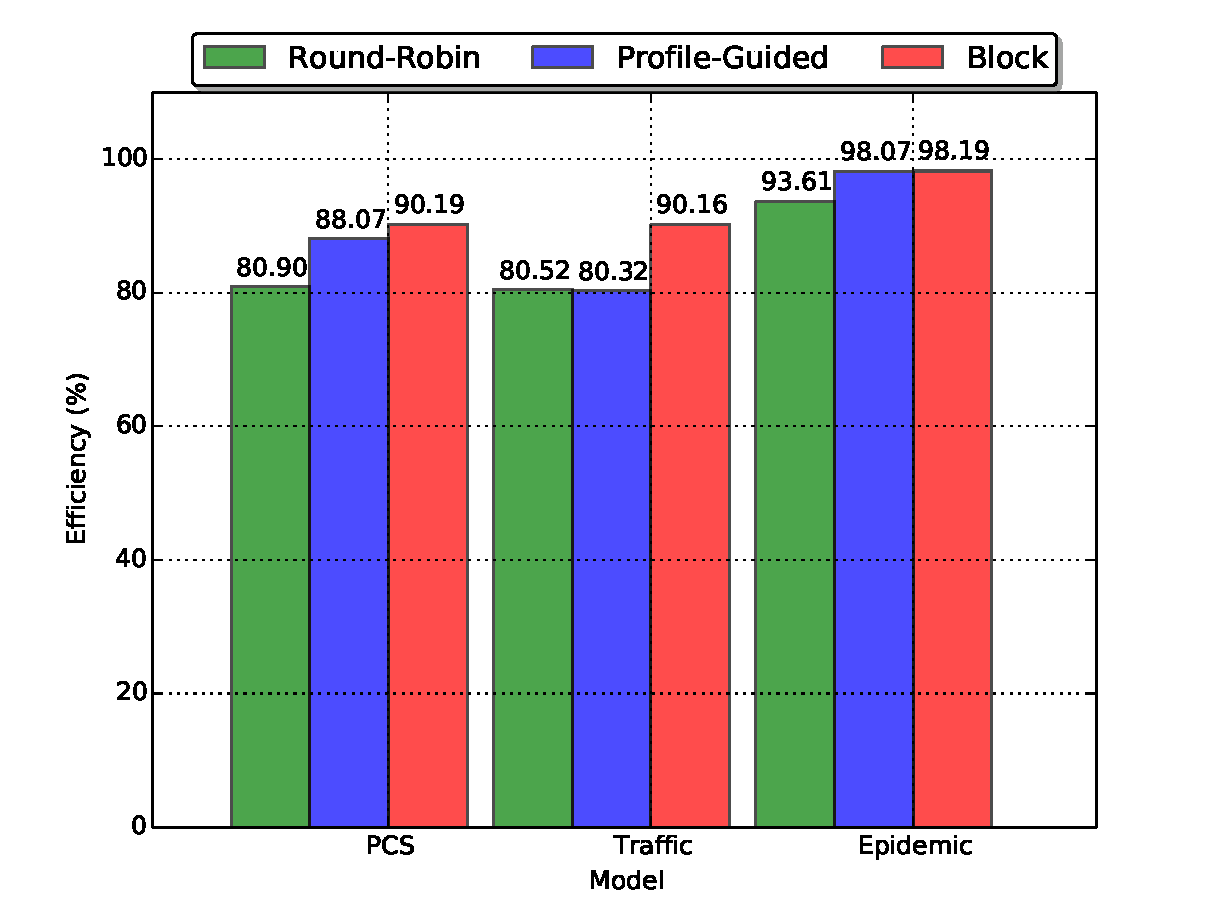
\includegraphics[width=\textwidth,keepaspectratio,quiet]{figs/partitioning_communication/partitioning_efficiency_8node.pdf} \\
      Efficiency \\
    \end{center}
  \end{minipage}
  \centering
  \begin{minipage}{.5\textwidth}
    \begin{center}
      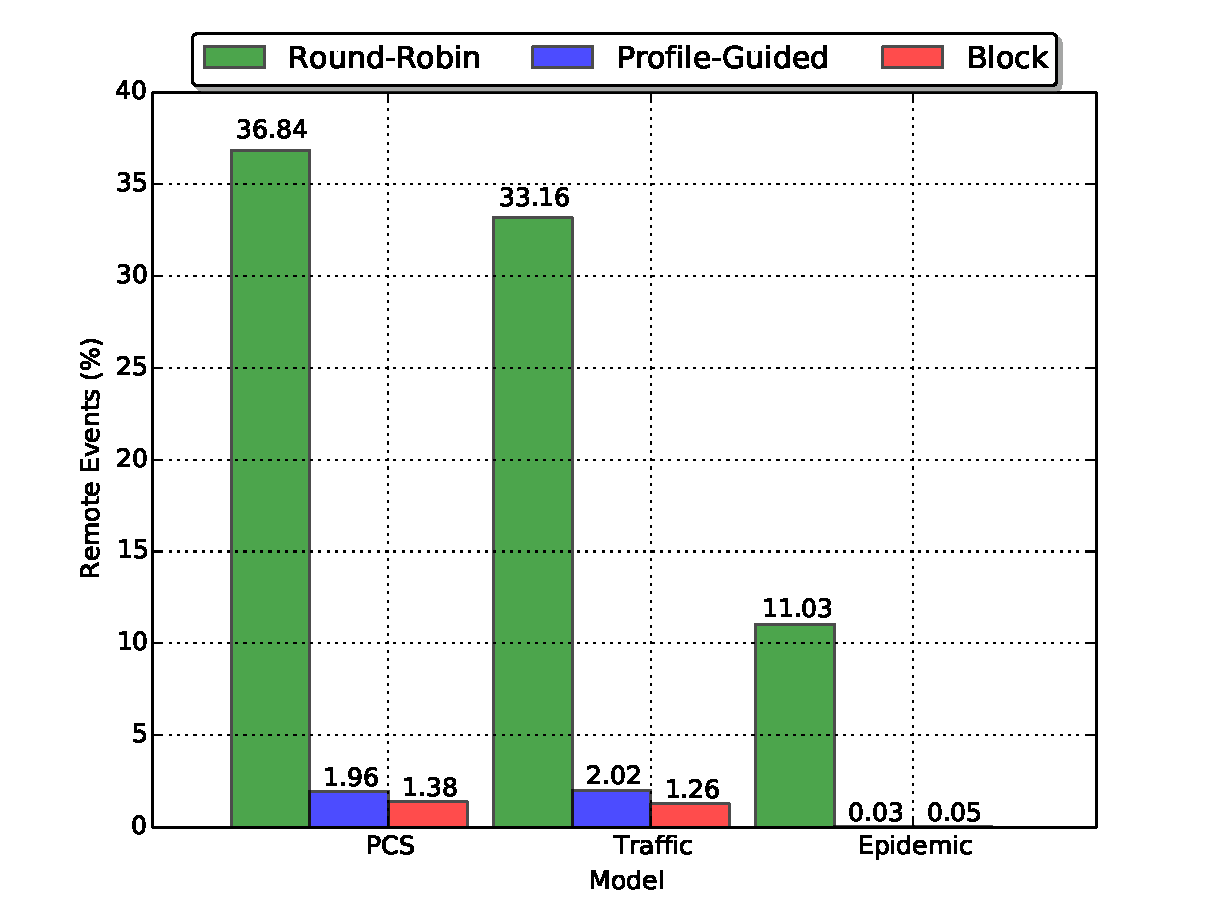
\includegraphics[width=\textwidth,keepaspectratio,quiet]{figs/partitioning_communication/partitioning_premote_8node.pdf} \\
      \% Remote Events \\
    \end{center}
  \end{minipage}
  \caption{Interprocess Partitioning: 8 Node Cluster}\label{partitioning_8node}
\end{figure}

For all models, the partitioning method that results in the highest event rate is block partitioning
and the second highest profile-guided partitioning.  In general, the best partitioning method
decreases remote communication the most which also results in the best efficiency.

\subsection{Aggregate Message Count}

MPI implementations are usually designed for coarse-grained parallelism and optimized for large
message sizes.  Parallel discrete event simulation is inherently fine-grained and the event sizes
are usually small which makes it less suitable for MPI.  To coarsen the granularity, messages that
are sent to the same destination process can be aggregated at the sender and split at the receiver.
By aggregating messages destined for the same process, some of the communication overheads can be
minimized.  Although the latency of each individual message may be increased, the total number of
messages that share the same latency will be larger than one.

\subsubsection{Message Aggregation Implementation}

The individual messages are aggregated into a single aggregate message until the aggregate message
contains $N$ individual messages or until a control message is included.  A control message could be
a GVT token, a termination token, a GVT update message, or termination status update message.

The combined message is started with a header which includes the number of individual messages and
the lengths of each individual message.  The location of each individual message can be found by
adding the length of the header with the length of the previous message and the length of the header
is easily determined by knowing how many individual message there are.  Figure
\ref{aggregate_format} illustrates the format of the aggregated message with the sizes of each
field.

\begin{figure}
    \centering
    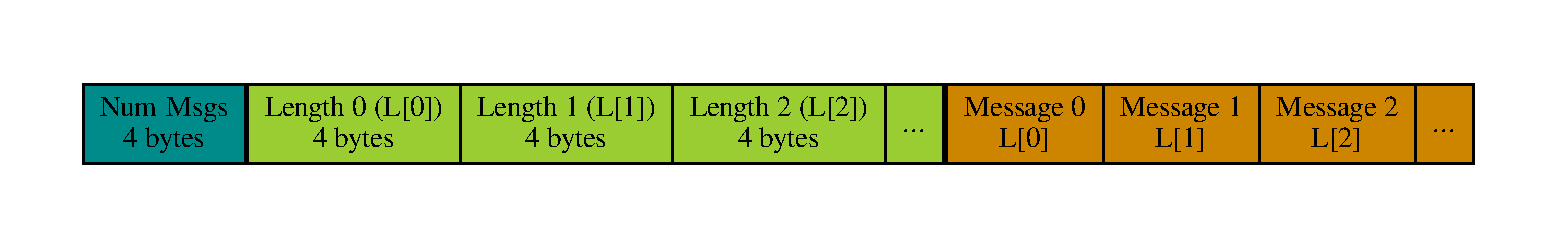
\includegraphics[width=0.8\textwidth,quiet]{figs/graphviz/aggregation_format.pdf}
    \caption{Aggregate Message Packet Format}\label{aggregate_format}
\end{figure}

\noindent
The size of the aggregated messages in bytes are:

$$ 4 * (N + 1) + \sum_{n=0}^{N-1} length[n] $$

\noindent
A message count approach was chosen over size base approach in \textsc{warped2} since the size of
the serialized messages would not be known until they the serialization is performed.  Because of
this, a separate temporary buffer would be needed for each individual message before copying them
into a new aggregated buffer, which could be very costly.  Also, smaller message sizes could be
possible by eliminating the need for a header by separating individual messages with a special
token.  However, a binary serialization method is used in \textsc{warped2} which makes it impossible
to split and deserialize the individual messages at the receiving process.

\subsubsection{Message Aggregation Analysis}

The plots in Figures \ref{aggregate_eventrate} show how various message aggregate sizes affect event
rate the PCS, traffic, and epidemic models.  The results are also plotted for different state saving
periods since different state saving period tends to have a significant impact on message
aggregation behavior.  The results for PCS and Traffic indicate that just a small number of
aggregated messages can have a significant impact on increasing the event rate and the efficiency as
long as the state saving period is not too high.  With a larger state saving period, the performance
drops off much faster with an increasing number of aggregated messages than with a small state
saving period.

\begin{figure}
  \begin{minipage}{.5\textwidth}
    \begin{center}
      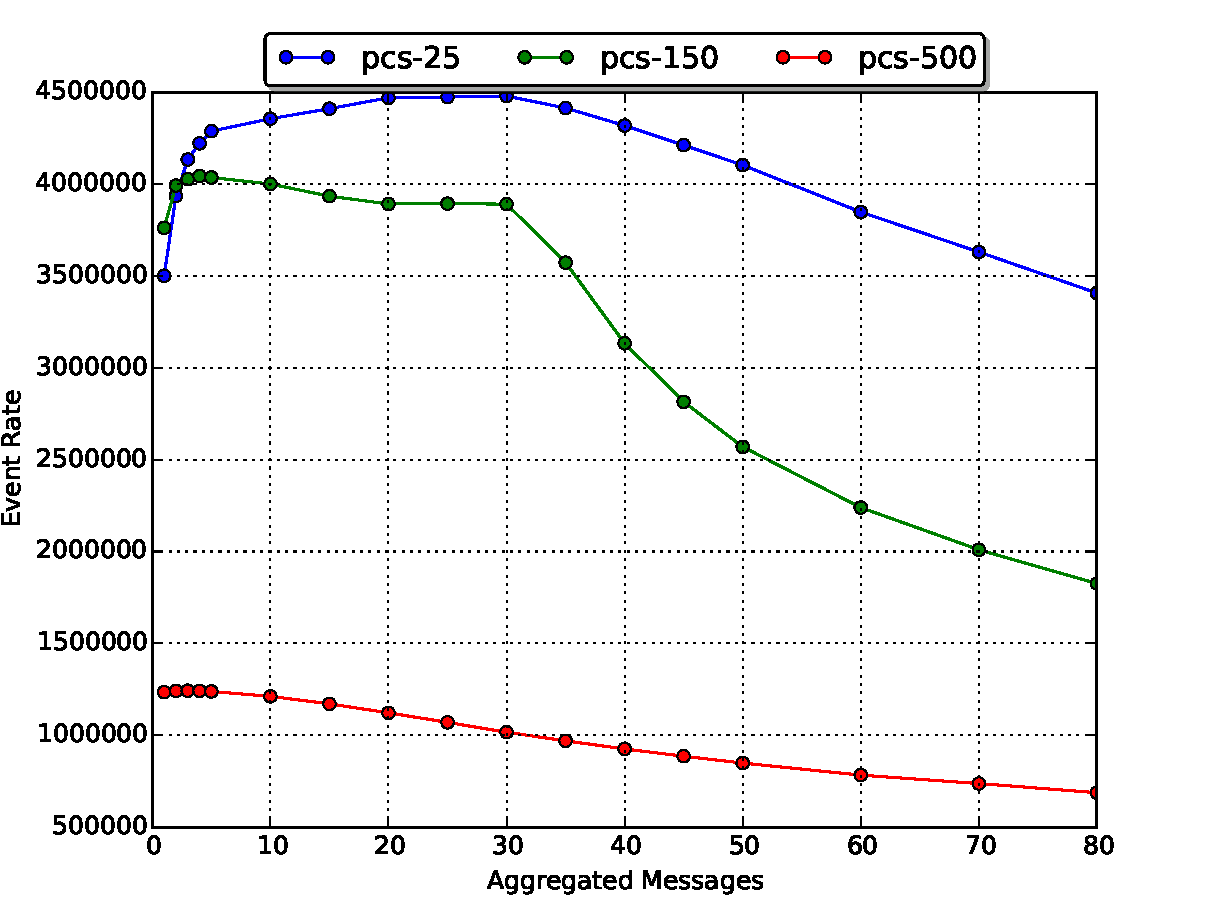
\includegraphics[width=\textwidth,keepaspectratio,quiet]{figs/partitioning_communication/aggregate_pcs_eventrate.pdf} \\
      PCS \\
    \end{center}
  \end{minipage}%
  \hfill
  \begin{minipage}{.5\textwidth}
    \begin{center}
      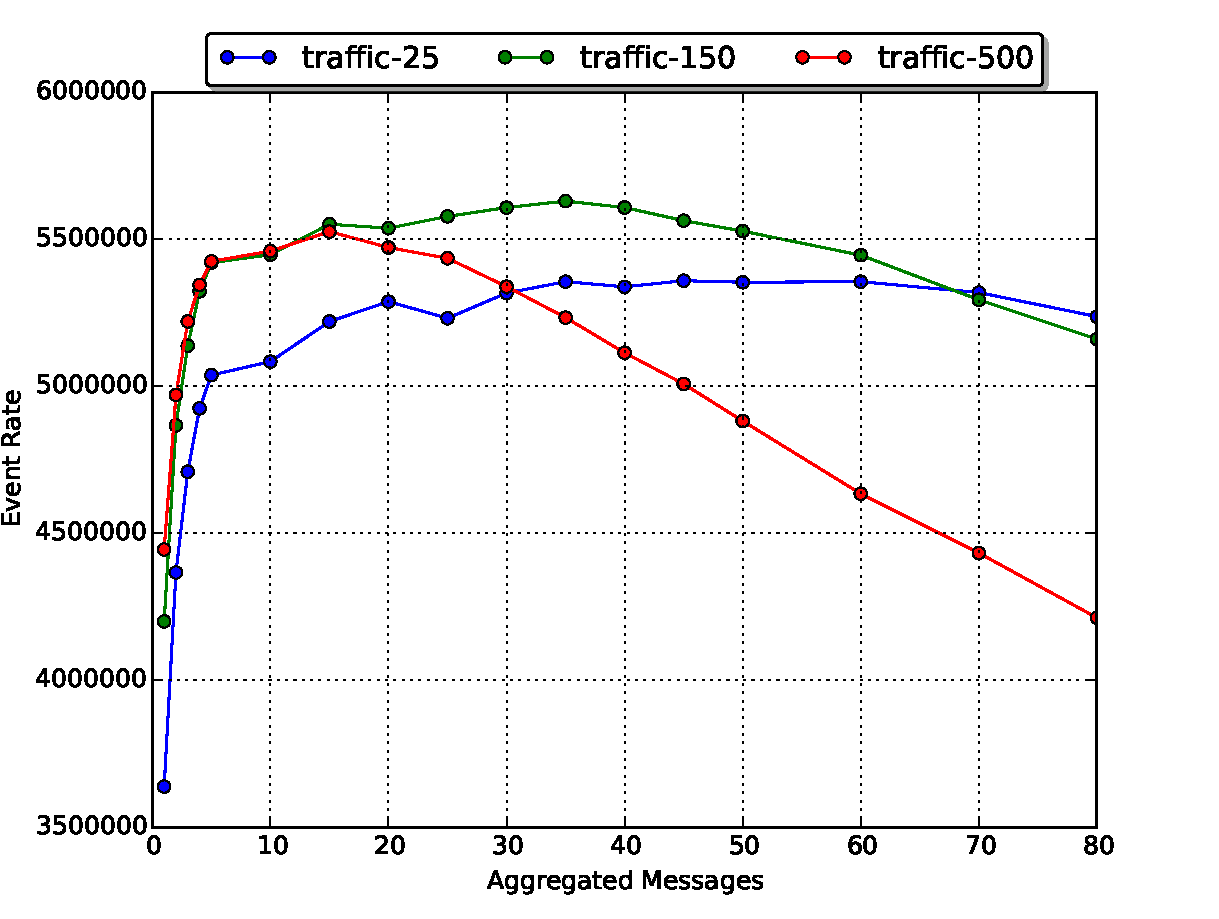
\includegraphics[width=\textwidth,keepaspectratio,quiet]{figs/partitioning_communication/aggregate_traffic_eventrate.pdf} \\
      Traffic \\
    \end{center}
  \end{minipage}
  \centering
  \begin{minipage}{.5\textwidth}
    \begin{center}
      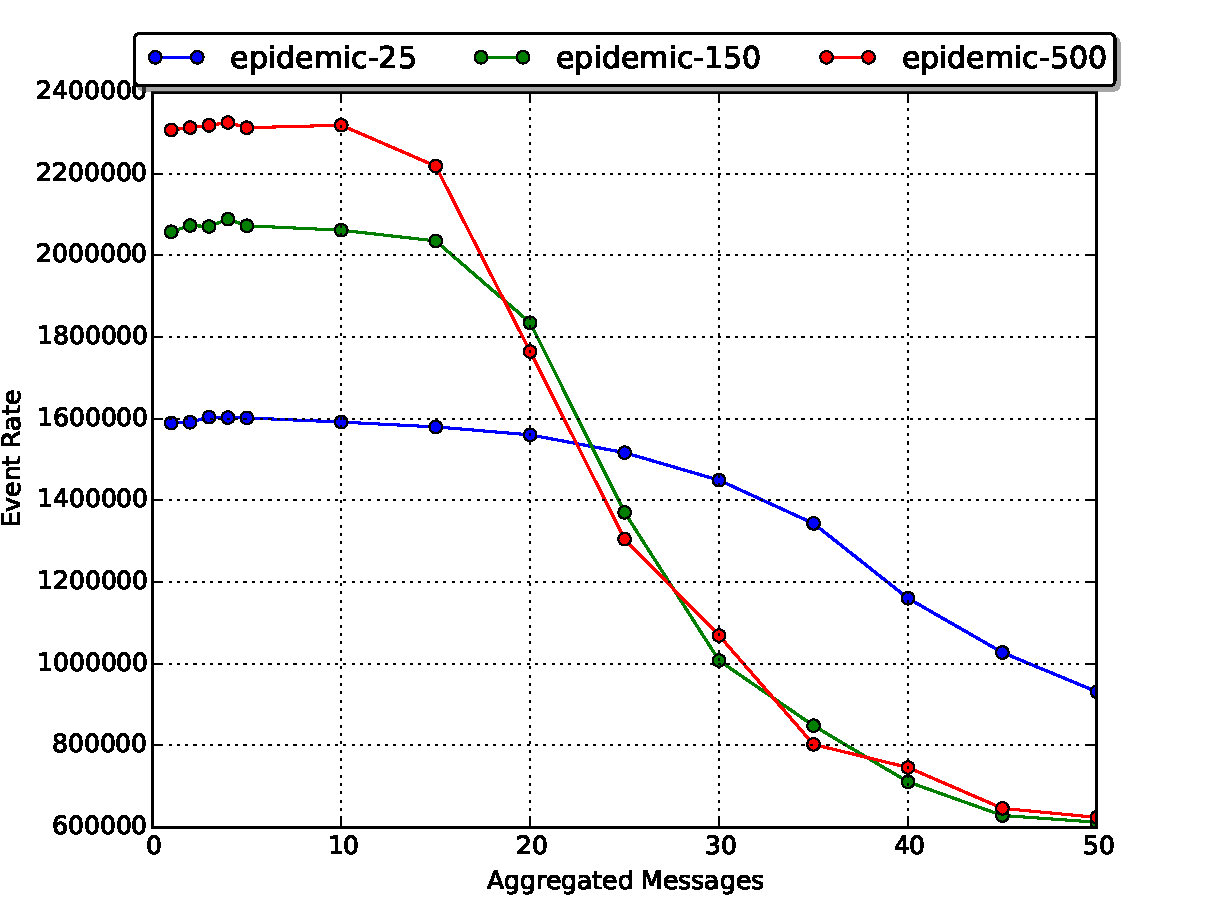
\includegraphics[width=\textwidth,keepaspectratio,quiet]{figs/partitioning_communication/aggregate_epidemic_eventrate.pdf} \\
      Epidemic \\
    \end{center}
  \end{minipage}
  \caption{Aggregate Messages: Event Rate}\label{aggregate_eventrate}
\end{figure}

\begin{figure}
  \begin{minipage}{.5\textwidth}
    \begin{center}
      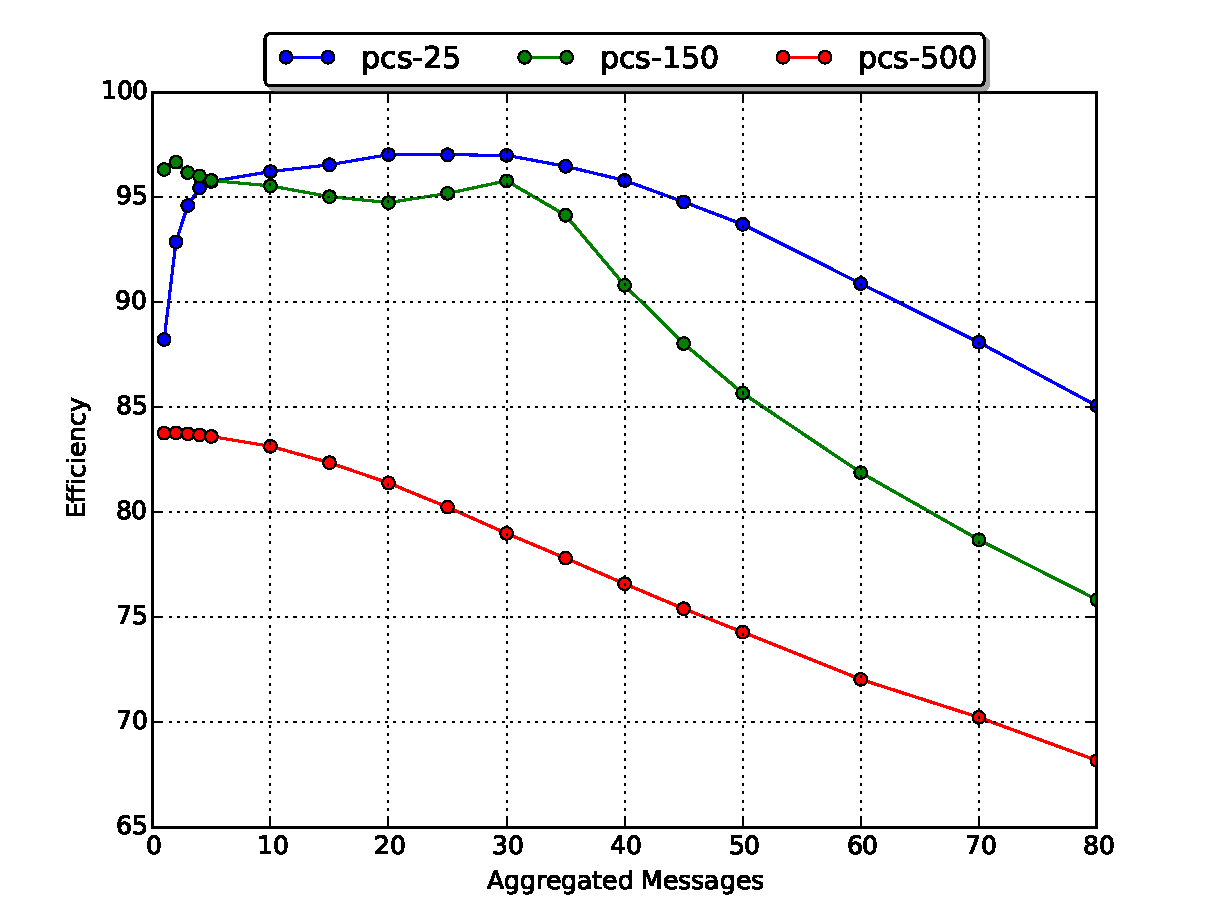
\includegraphics[width=\textwidth,keepaspectratio,quiet]{figs/partitioning_communication/aggregate_pcs_efficiency.pdf} \\
      PCS \\
    \end{center}
  \end{minipage}%
  \hfill
  \begin{minipage}{.5\textwidth}
    \begin{center}
      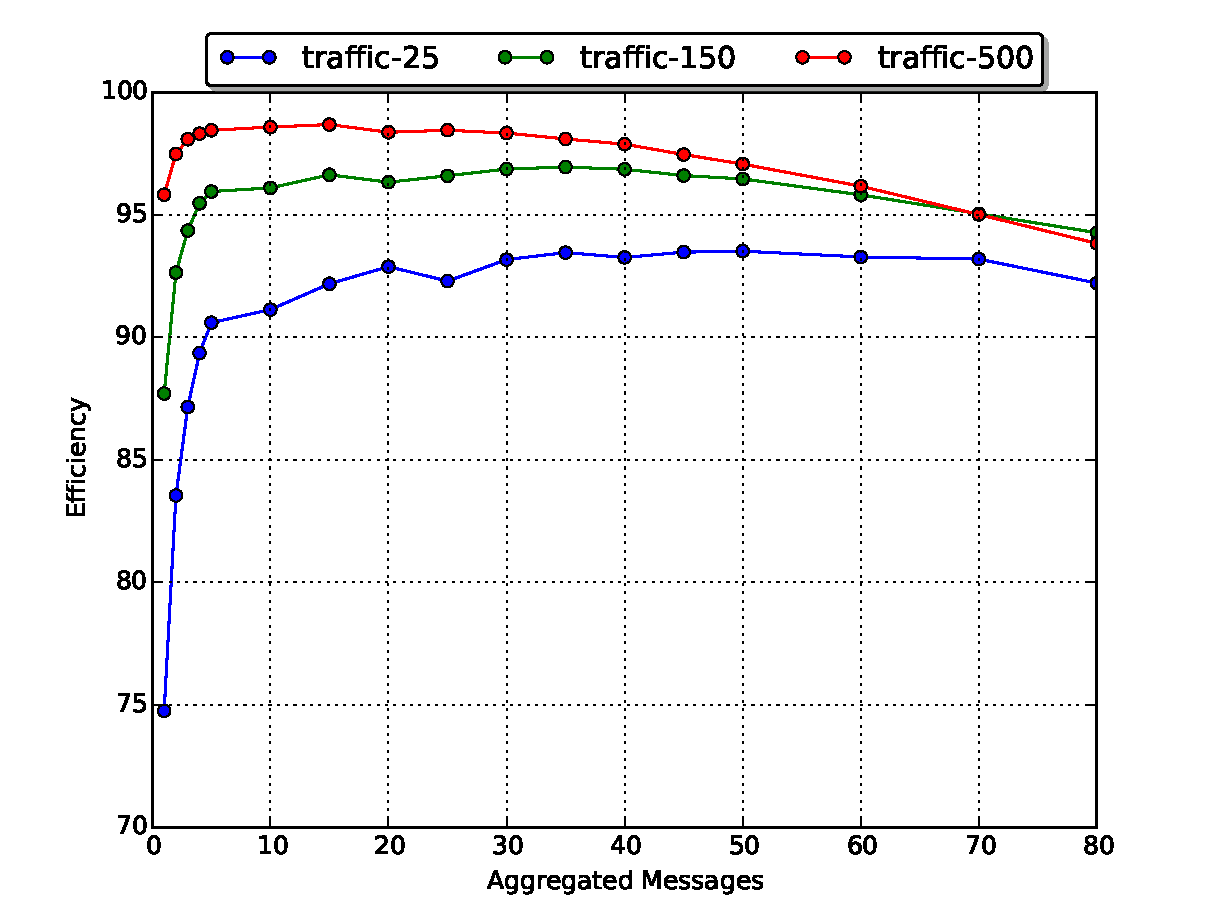
\includegraphics[width=\textwidth,keepaspectratio,quiet]{figs/partitioning_communication/aggregate_traffic_efficiency.pdf} \\
      Traffic \\
    \end{center}
  \end{minipage}
  \centering
  \begin{minipage}{.5\textwidth}
    \begin{center}
      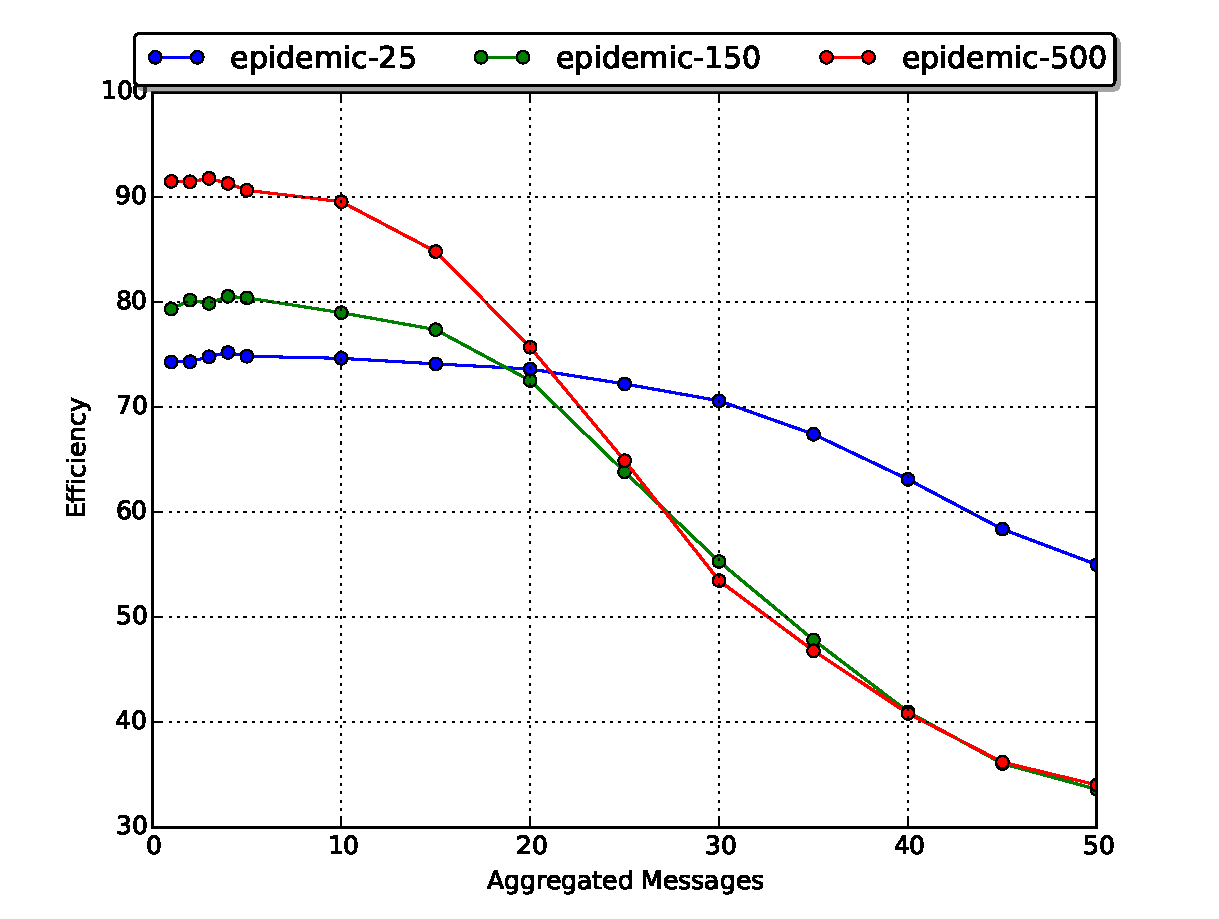
\includegraphics[width=\textwidth,keepaspectratio,quiet]{figs/partitioning_communication/aggregate_epidemic_efficiency.pdf} \\
      Epidemic \\
    \end{center}
  \end{minipage}
  \caption{Aggregate Messages: Efficiency}\label{aggregate_efficiency}
\end{figure}
  
The behavior of message aggregation on performance and efficiency can be described by realizing that
it works better in cases that remote events are sent at faster rates.  Figure \ref{remote_ssp}
illustrates how the state saving period can change the rate at which remote events are sent.  As the
state saving period is increased the remote event rate tends to decrease.  Also, it shows that the
epidemic model has a much slower rate than PCS and traffic models which explains why message
aggregation doesn't have any benefit for epidemic.

\begin{figure}
  \centering
  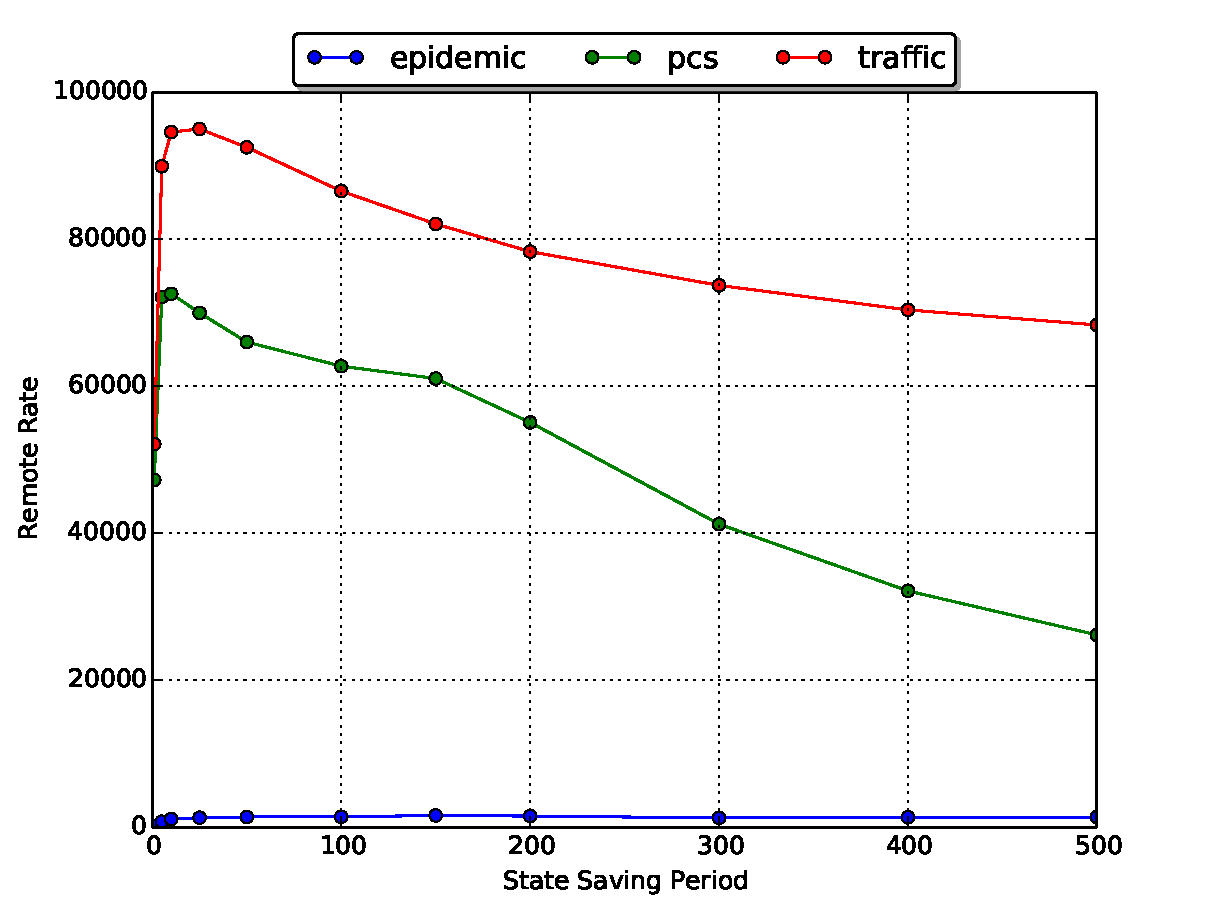
\includegraphics[width=0.5\textwidth,keepaspectratio,quiet]{figs/state_saving/beowulf/remote_rate.pdf} \\
  \caption{Remote Rate versus State Saving Period}\label{remote_ssp}
\end{figure}

If remote events are sent at a faster rate, then the aggregated messages can be sent faster and
individual events are not temporarily queued as long.  If the amount of time that the individual
events are queued is small compared to the network latency, then aggregation will have much benefit
but if the time is too long, then the queuing delay will slow down communication.

The total latency is a combination of the queuing delay and network latency.  Minimizing the total
latency of the individual messages is the key to minimizing rollbacks and increasing the efficiency.
By increasing the number of messages aggregated together, the network latency per individual message
becomes smaller because the latency is shared between the messages but the queueing delay increases.
For this reason, a small number of messages aggregated together may improve efficiency if the
queuing delay is small, but when the number of messages gets too high then the queuing delay gets
too large and very long rollbacks may occur.

\section{Scaling up the Simulation Model}

All previous simulation results have been from simulation models that were configured for 10,000
LPs.  This section analyzes the behavior of the simulations when the number of LPs are scaled up to
larger numbers on an 8 node cluster.  Figure \ref{scaling} shows how the traffic and PCS simulation
model scale up with 5 messages aggregated and no message aggregation.

\begin{figure}
  \begin{minipage}{.5\textwidth}
    \begin{center}
      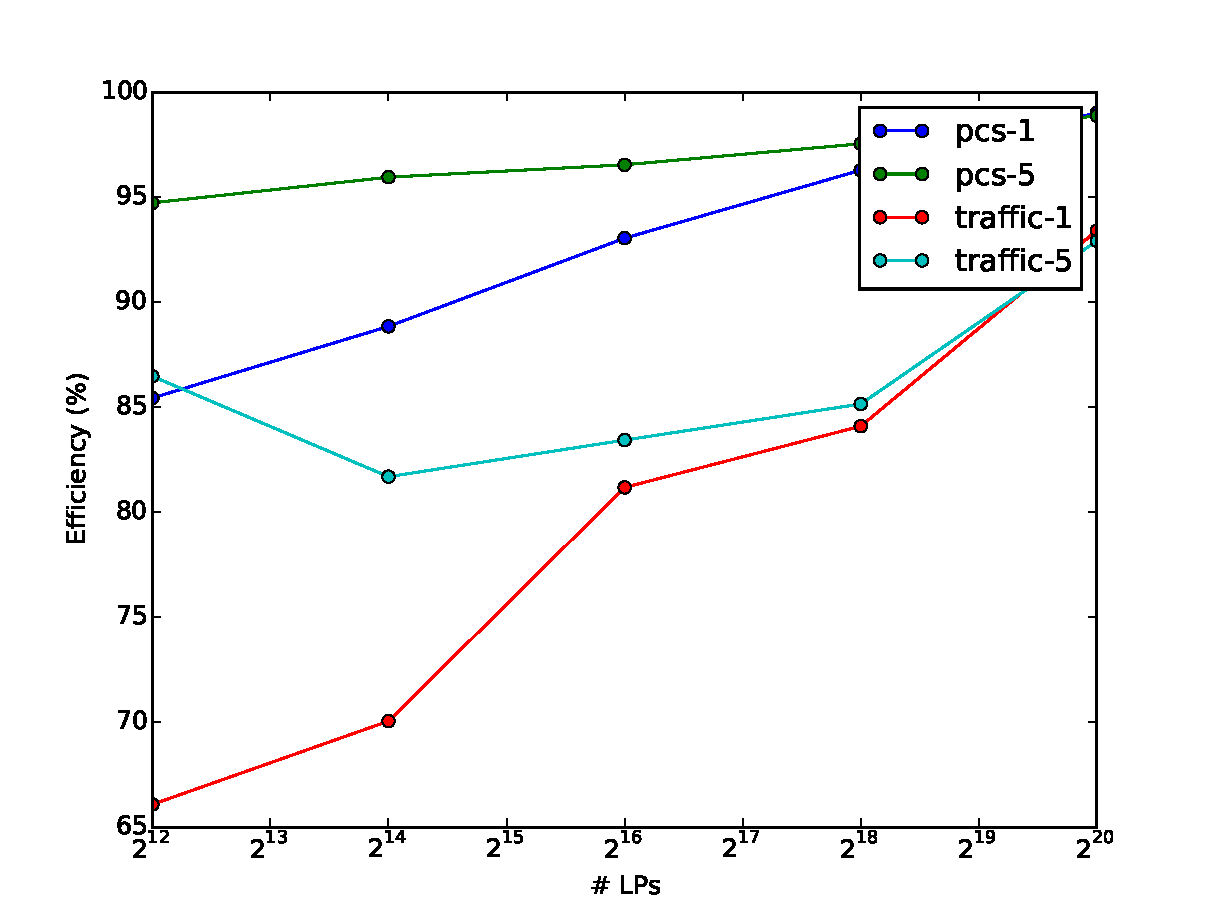
\includegraphics[width=\textwidth,keepaspectratio,quiet]{figs/scale/scale_efficiency.pdf} \\
      Efficiency \\
    \end{center}
  \end{minipage}%
  \hfill
  \begin{minipage}{.5\textwidth}
    \begin{center}
      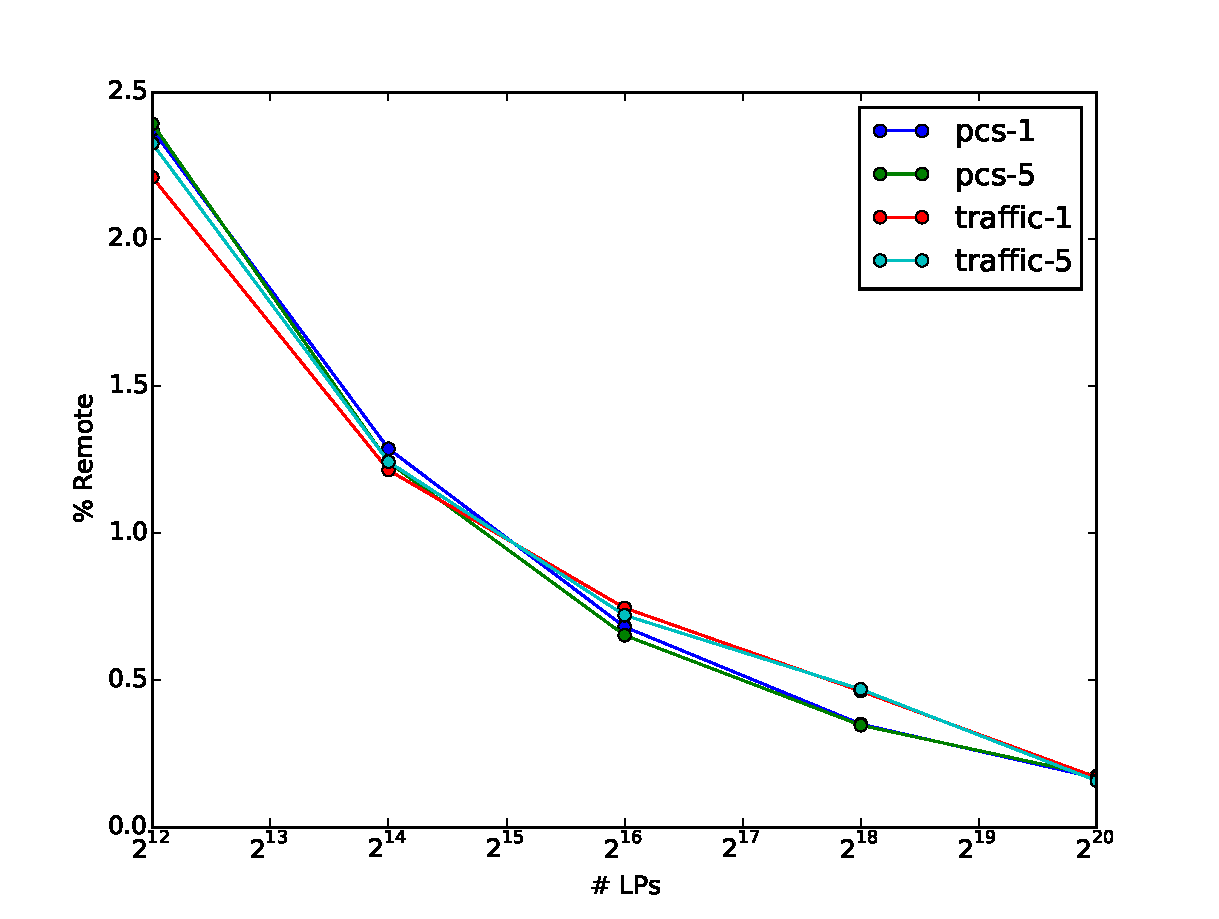
\includegraphics[width=\textwidth,keepaspectratio,quiet]{figs/scale/scale_premote.pdf} \\
      \% Remote Events \\
    \end{center}
  \end{minipage}
  \centering
  \begin{minipage}{.5\textwidth}
    \begin{center}
      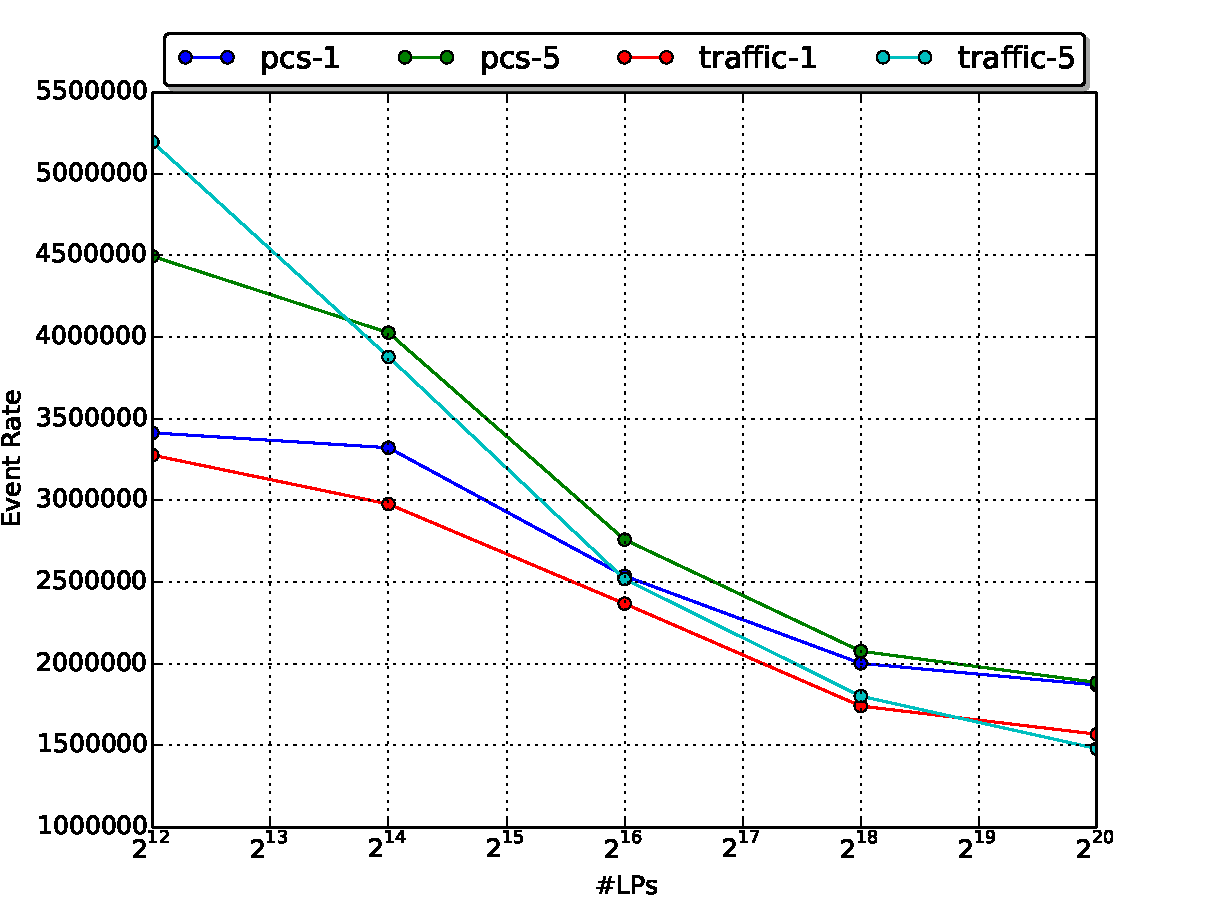
\includegraphics[width=\textwidth,keepaspectratio,quiet]{figs/scale/scale_event_rate.pdf} \\
      Event Rate \\
    \end{center}
  \end{minipage}
  \caption{Scaling \#LPs on a Cluster}\label{scaling}
\end{figure}

It appear, from these results, that as these models are scaled up, the benefit of aggregated
messages decreases.  That is, the efficiency and event rate for aggregate versus individual messages
converge with more LPs.

In general, whether aggregate messages are used or not, scaling up the number of LP always has the
same effect.  The efficiency increases significantly due to the work being spread out among more
LPs.  Statistically, the odds that two LPs will send events to the same LP and the receiving LP will
process them out of order diminishes with a scaled simulation model.  Also, each process processes
events for a larger subset of the LPs.  If the simulation model can be partitioned well in any way,
scaling up will only make partitioning more effective since the cross-partition communication will
remain small as the partition size grows.  This is what ultimately reduces the reduction in the
percentage of events that are remote.

The event rate tends to decrease, however as the number of LPs increases.  The reason for this is
that each worker thread will have to use a larger percent its time to fossil collect LPs instead of
processing events.



\chapter[Event Scheduling]{Event Scheduling and Processing in \textsc{warped2}}\label{warped2_ds}

\section{Pending Event Set Data Structures}

The pending event set is the set of events that are ready to be processed at any given time.  Every
process contains a logically separate pending event set for a dedicated set of LPs.  Events that are
being sent to an LP that is local to the process are directly inserted into the pending event set.
Events that must be sent to a remote process are inserted into a remote event send queue where the
manager thread will remove it, form an event message and send the message to the receiving process.
The manager thread at the receiving process will then unpack the message and insert it into the
pending event set.  The pending event set is made up of a queue for each LP known as an
\emph{unprocessed queue} which is directly accessible from all threads and allows for the sending of
events.

The unprocessed queue contains both positive events and anti-messages and remains sorted at all
times.  The anti-messages are given priority over their positive counterparts so that the
anti-messages are always processed first and any unnecessary rollbacks can be prevented which
could create a chain of rollbacks that could cause instability \cite{lubachevsky-89}.  To avoid
any unnecessary copying from the simulation model to the kernel and with the kernel, the
unprocessed queue only contains pointers to the unprocessed events which are passed in by the
simulation model.

A second type of data structure, an \emph{LTSF (Lowest TimeStamp First) Queue}, provides order among
events from multiple LPs.  At most, a single event from each LP is \emph{scheduled} into a single
LTSF queue.  Scheduling an event to an LTSF queue means only inserting a pointer to an event into
the LTSF queue with no removal from the unprocessed queue.  Every process has one or more LTSF
queues which the worker threads obtain the lowest timestamped event to process.

A third type of data structure is also used to keep track of the events that have been scheduled or
are currently being processed but organized by receiving LP.  It is used for two main reasons.
First, when inserting an event into the receiving LPs unprocessed queue, it provides a way to
determine if a smaller event has already been scheduled for the LP.  The new event can then be
scheduled in place of the already scheduled event.  Second, it serves to prevent multiple worker
threads from processing events from the same LP which could cause out of order committing of events
without rolling back as would be necessary.  Figure \ref{pending_event_set} illustrates the pending
event set data structures in \textsc{warped2}.

\begin{figure}
    \centering
    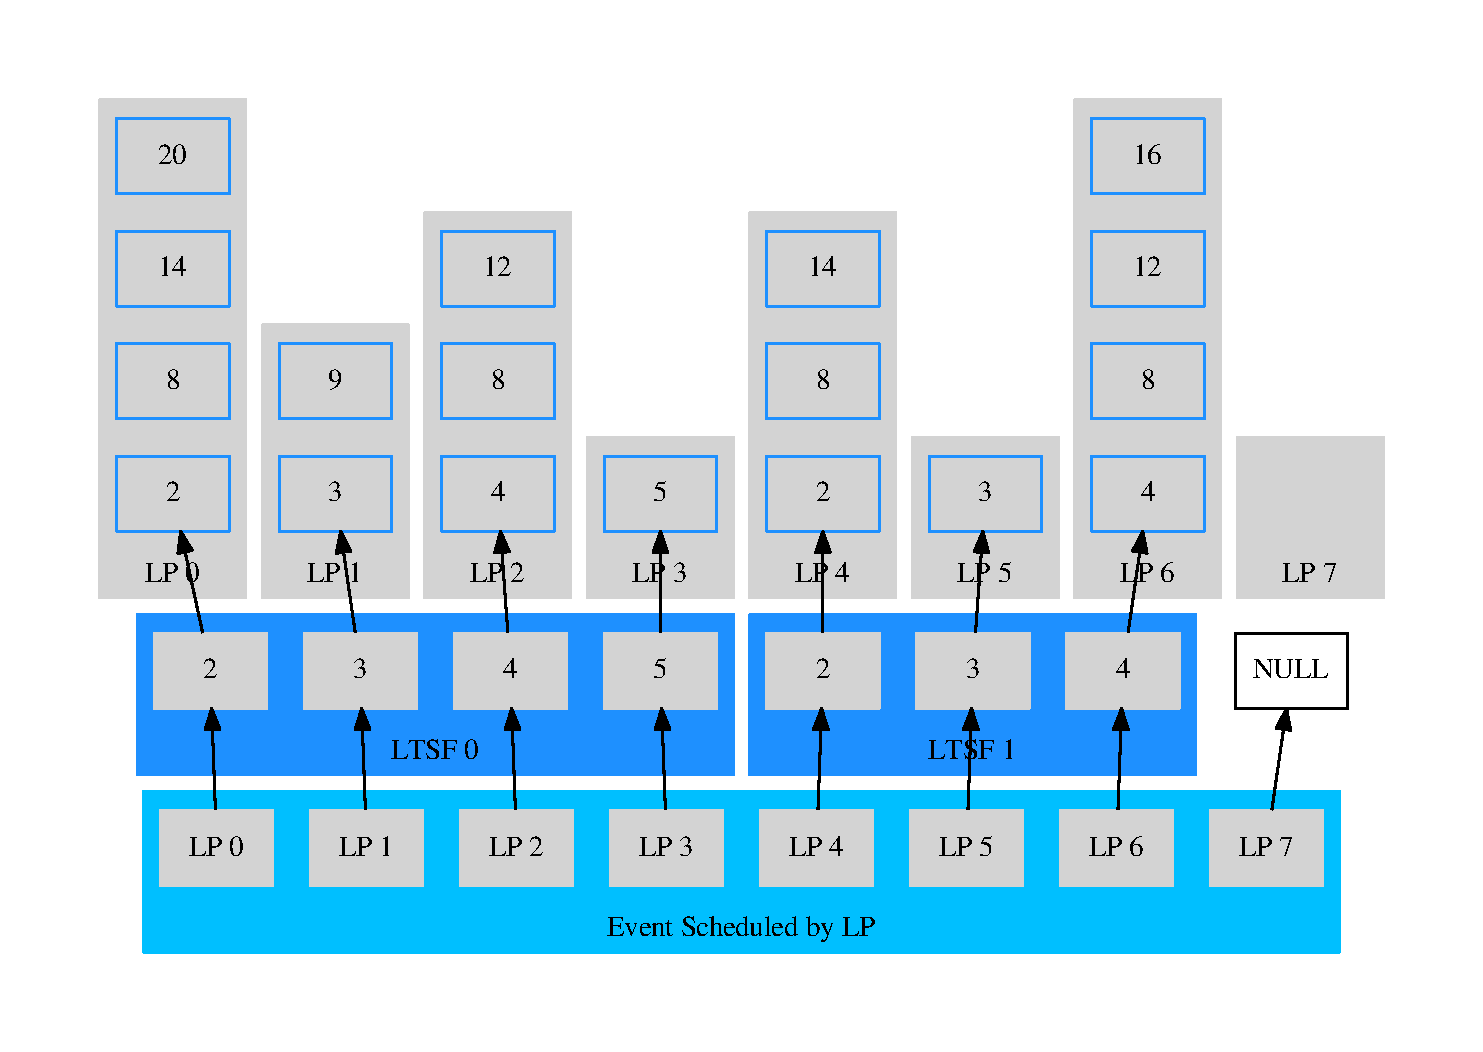
\includegraphics[width=0.75\textwidth,quiet]{figs/graphviz/pending_event_set.pdf}
    \caption{\textsc{warped2} Pending Event Set Data Structures}\label{pending_event_set}
\end{figure}

\section{Processing Events}

One or more of the worker threads are assigned to each LTSF Queue to process events from and they
all follow the exact same procedure.  First, an event is removed from an LTSF queue to be processed
but remains in the unprocessed queue until it is completely processed or canceled out.  The event
is first checked against the last processed event of the receiving LP to see if it is a straggler,
and rolled back if necessary.  An anti-message is also considered to be a straggler if its positive
counterpart was the last processed event for the LP.  If the event is an anti-message, the positive
counterpart cannot be assumed to be in the LPs unprocessed queue.  If the positive event is present
then it is canceled out but if it is not present then the anti-message remains in the unprocessed
queue.  In both cases, an attempt to reschedule a new event to the LTSF queue occurs and the worker
thread continues to the next event.  If the next event to be processed is positive then it is
processed normally, the state of the LP is saved, and new events are sent to other LPs.  The event
is then moved into the processed queue and a new event is scheduled into the LTSF queue.  To
summarize, the worker thread processing loop is shown in pseudocode in Algorithm
\ref{warped2_processing}.

\begin{algorithm}
\DontPrintSemicolon
\SetKw{Continue}{continue}
\SetKwFunction{getNextEvent}{getNextEvent}

    \While{termination not detected}{
        \nlset{1} $e \gets \getNextEvent{}$\;
        $lp \gets$ receiver of $e$\;\;

        \If{$e <$ last processed event for $lp$}{
            rollback $lp$\;
        }
        \;
        \If{$e$ is an anti-message}{
            cancel event with $e$ if possible\;
            \nlset{3} schedule new event for $lp$\;
            \Continue\;
        }
        \;
        process event $e$\;
        save state of $lp$\;
        \nlset{2} send new events\;
        move $e$ to processed queue\;
        \nlset{3} replace scheduled event for $lp$\;
    }

\caption{\textsc{warped2} Main Event Processing Loop}\label{warped2_processing}
\end{algorithm}

%% Sending events
When events are inserted into the unprocessed queues, they are compared to the currently scheduled
event for the LP.  If there is no currently scheduled event or the new event is less than the
currently scheduled event, then the new event is scheduled to prevent a rollback from occurring.

\subsection{Ordering of Events}

The Time Warp mechanism assumes that every event is labeled with a totally ordered clock value based
on virtual time \cite{jefferson-85}.  This is important so that causal dependencies are preserved
and so that simulation results are deterministic\cite{ronngren-99}.  To ensure this,
\textsc{warped2} uses a 4-tuple scheme which provide a total ordering of events:

\begin{enumerate}
    \item Receive Time
    \item Send Time
    \item Sender LP Name
    \item Generation
\end{enumerate}

\noindent %% tiebreaking
The last three serve as a tie breaker for simultaneous receive times.  The send time is necessary to
ensure correct causal dependencies.  It is analogous to a Lamport logical clock\cite{lamport-78} in
real time distributed systems but for virtual time systems.  The send time will work as long as LPs
only send a single event with the same send time, receive time, and receiver LP.  Otherwise, a more
strict ordering of sends would be required.  However, \textsc{warped2} forbids this behaviour in the
simulation model.  The sender LP name is necessary to ensure that order is determined between events
received with the same receive time and send time from different senders.  Without it, it is
possible that different results could occur on different runs of the simulation \cite{ronngren-99}.
The generation is necessary for distributed memory systems to differentiate between the same events
which could be resent after rolling back \cite{ronngren-99}.  In \textsc{warped2} it is implemented
as a single counter per LP and keeps track of the number of events that have been sent from the LP.
The count is then tagged in the event when it is sent and used for comparison at the receiver.

\section{Performance Tuning Parameters}

To allow \textsc{warped2} to run on a large range of machines with different architectures and
characteristics, a number of parameters are provided for the user to tune the simulation mechanism
for their needs.  In the current implementation, the four main parameters that will determine
performance on a single SMP machine are the number of worker threads, the number of LTSF Queues, the
LTSF partitioning method, and the state saving period.

\subsection{Worker Threads and LTSF Queues}

The number of worker threads that should be used will depend on the number of processors of the
machine so it is left as a tunable parameter.  \textsc{warped2} also allows the user to choose the
number of LTSF queues.  The user can specify any number of LTSF queues, however, it must be smaller
than the number of worker threads and also be a factor of the number worker threads.

If all worker threads share a single LTSF queue then a huge contention point is created and
performance will suffer.  At the opposite extreme, however, with all worker threads processing
events from a separate LTSF queue, the critical path of the simulation will be spread out and
the number of rollbacks can increase significantly.  The extent to which these matter varies
depending on the characteristics of the simulation model.  Furthermore, they may also vary as the
data structures and algorithms in \textsc{warped2} evolve to minimize contention.

The plots shown in Figure \ref{ltsf_analysis} illustrate the effects of increasing the number of
LTSF queues with 10 worker threads.

\begin{figure}
  \begin{minipage}{.5\textwidth}
    \begin{center}
      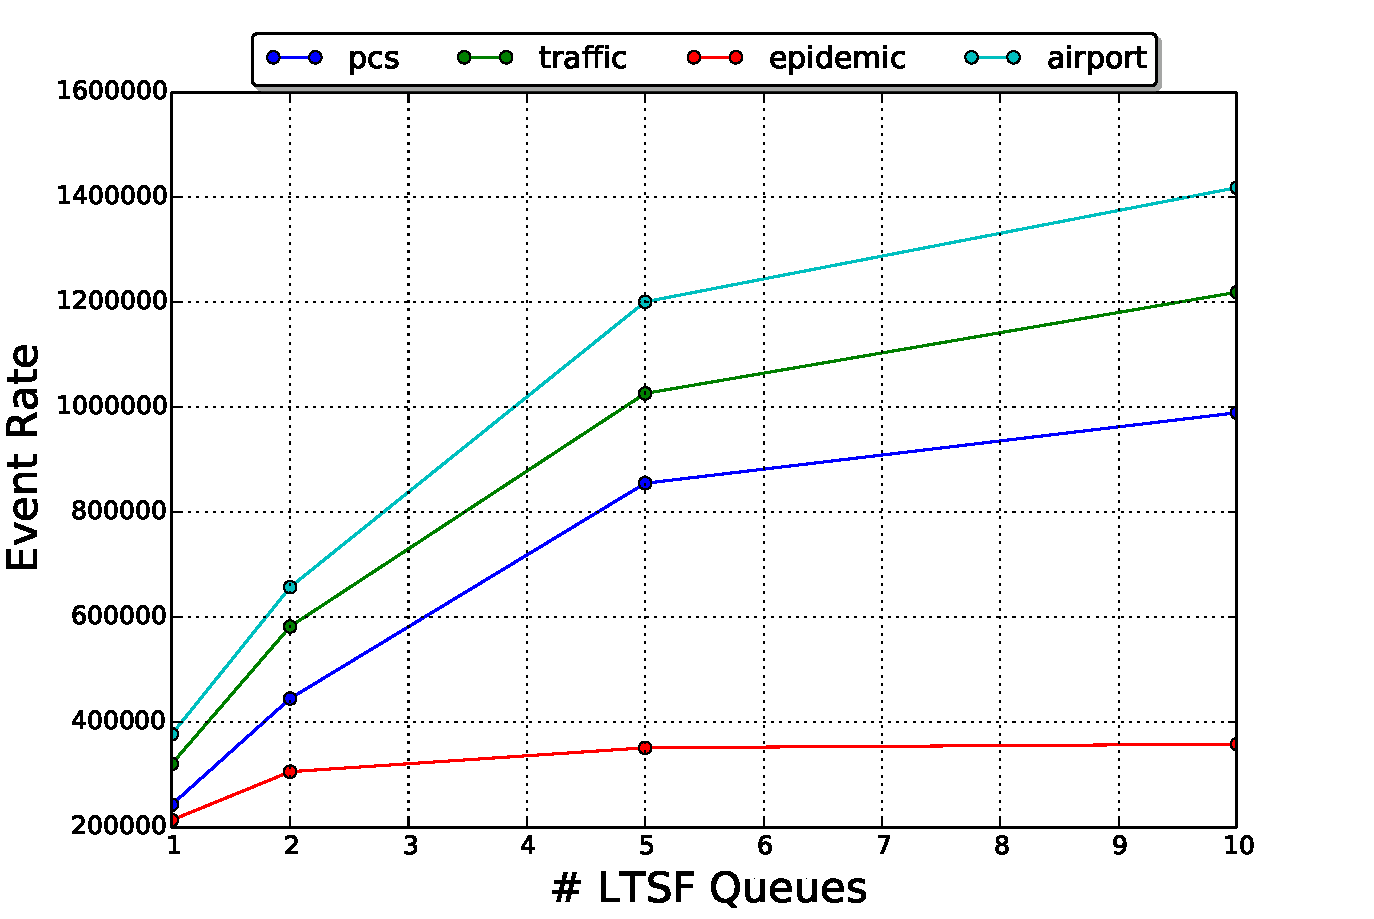
\includegraphics[width=\textwidth,keepaspectratio,quiet]{figs/pending_event_set/ltsf_event_rate.pdf} \\
      Event Rate \\
    \end{center}
  \end{minipage}%
  \hfill
  \begin{minipage}{.5\textwidth}
    \begin{center}
      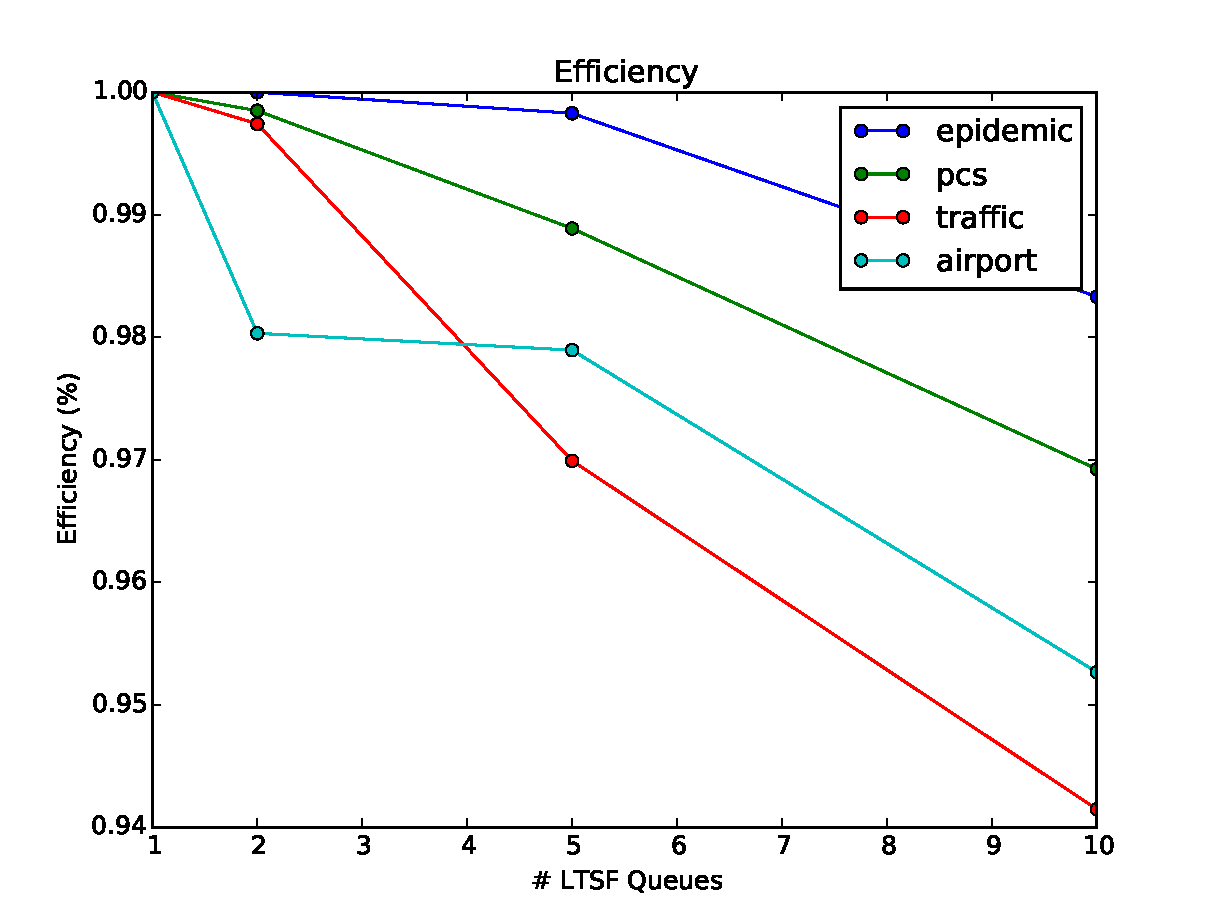
\includegraphics[width=\textwidth,keepaspectratio,quiet]{figs/pending_event_set/ltsf_efficiency.pdf} \\
      $Efficiency$ \\
    \end{center}
  \end{minipage}
  \caption{LTSF Queues: Performance on SMP Machine}\label{ltsf_analysis}
\end{figure}

Even though the number of total rollbacks increase with more LTSF queues, there is still a growing
speedup.  That means that the contention of the LTSF queue locks outweighs the extra time needed to
process more rollbacks.  By looking back at Figure \ref{warped2_processing}, we can see all the
critical points where worker threads can access the LTSF queues.  The lines with a number on the
margin indicate possible access to the LTSF queue.  For every event the LTSF queue is accessed at
least 3 times: \begin{inparaenum}[(1)] \item obtaining the next event, \item sending new events,
  and \item rescheduling new events \end{inparaenum}.  However, access to the LTSF cannot be
minimized further by refactoring.  Access to the LTSF queue will always be necessary to obtain the
next event and reschedule events and since the LTSF queue is only accessed while sending an event if
the event is a straggler, it will save a future access to the LTSF queue when the straggler is
scheduled and also prevent a rollback.

It is also worth noting that these simulation models are configured for only 10,000 LPs and with
larger models, the efficiency would be expected to be better.  Therefore, scaling up the number
of worker threads and LTSF queues together may not hinder performance if the simulation model
is also scaled up since efficiency and contention will not get worse.  

\subsection{LTSF Queue Partitioning}

The LPs can also be partitioned between LTSF queues in various ways just like partitioning between
processes.  In fact, there is only a single partitioning parameter for both levels of partitioning.
This makes sense because the LTSF queue partitioning will be negligible compared to the interprocess
but it allows the user to choose the LTSF queue partitioning directly on a single node simulation.

Figures \ref{ltsf_partitioning_beowulf} and \ref{ltsf_partitioning_bc} show the effects of LTSF
queue partitioning on simulation runtime and efficiency for the
Intel\textsuperscript{\textregistered} Xeon\textsuperscript{\textregistered} E5410 processor and
Intel\textsuperscript{\textregistered} Xeon\textsuperscript{\textregistered} X5675 processor,
respectively.

The simulations on the Intel\textsuperscript{\textregistered} Xeon\textsuperscript{\textregistered}
E5410 are configured with 8 LTSF queues, and 8 worker threads and the simulations on the 
Intel\textsuperscript{\textregistered} Xeon\textsuperscript{\textregistered} X5675 are configured
with 10 LTSF queues, and 10 worker threads.

\begin{figure}
  \begin{minipage}{.5\textwidth}
    \begin{center}
      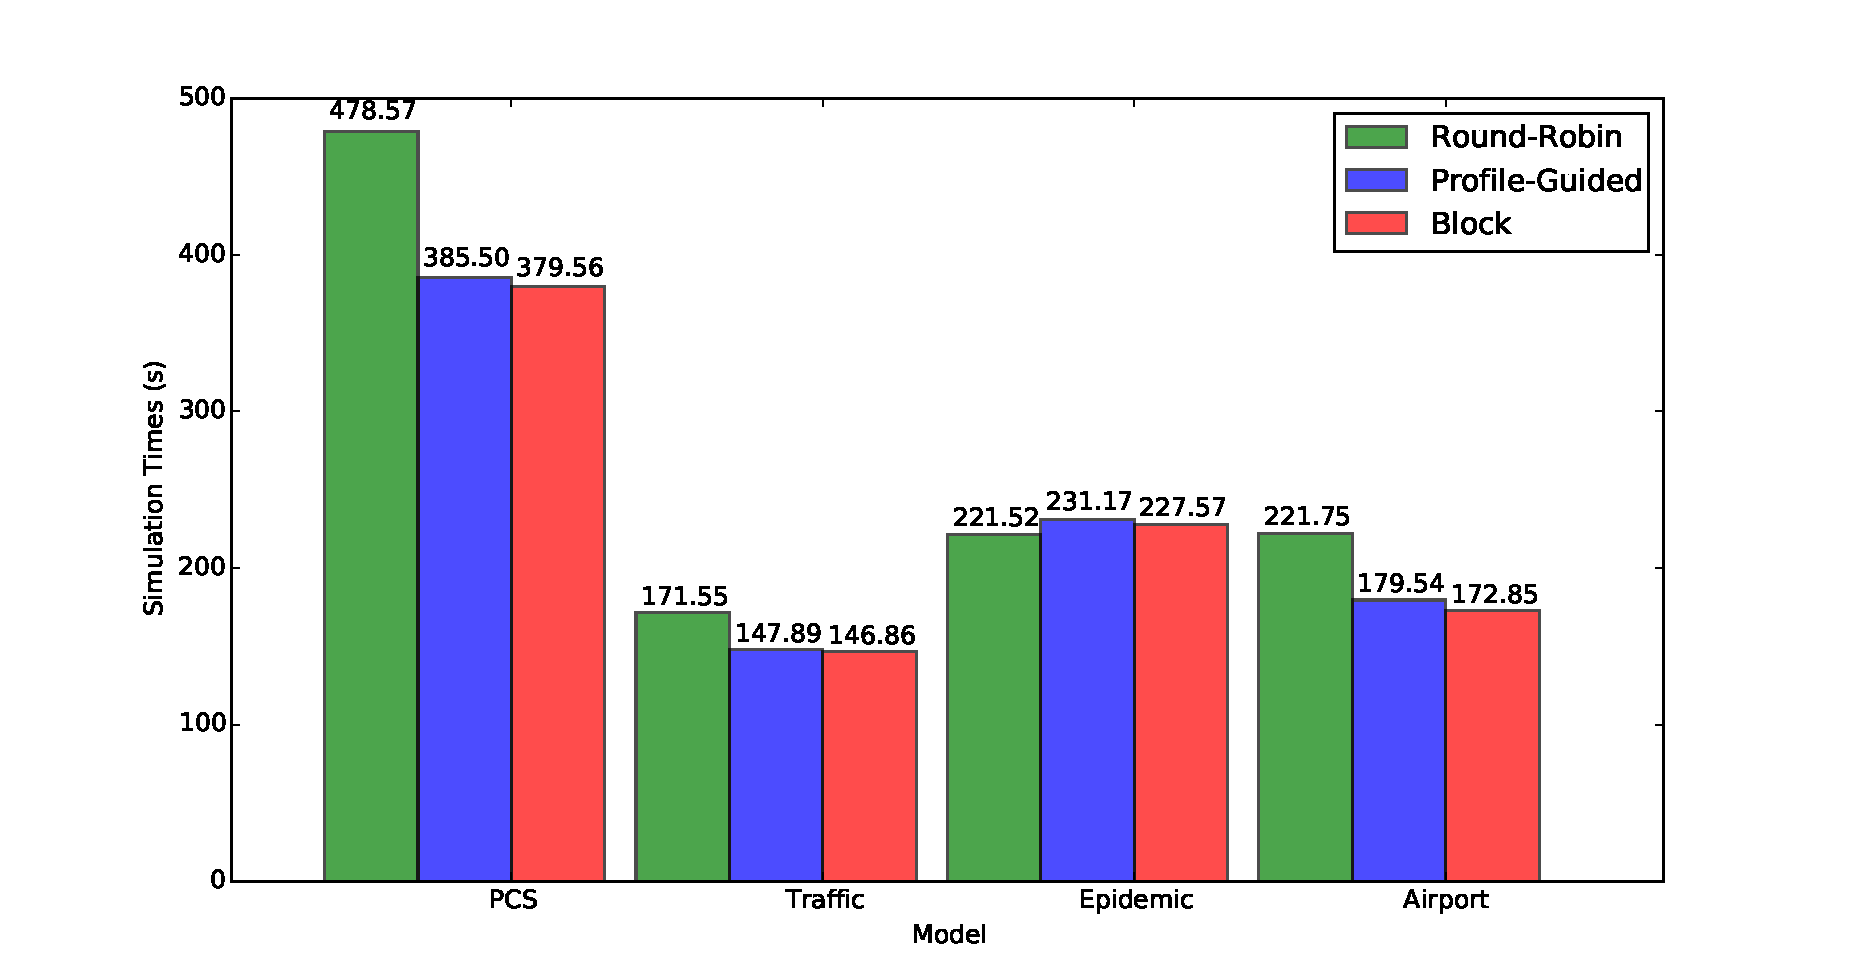
\includegraphics[width=\textwidth,keepaspectratio,quiet]{figs/partitioning_communication/partitioning_time_1node.pdf} \\
      Simulation Times (s) \\
    \end{center}
  \end{minipage}%
  \hfill
  \begin{minipage}{.5\textwidth}
    \begin{center}
      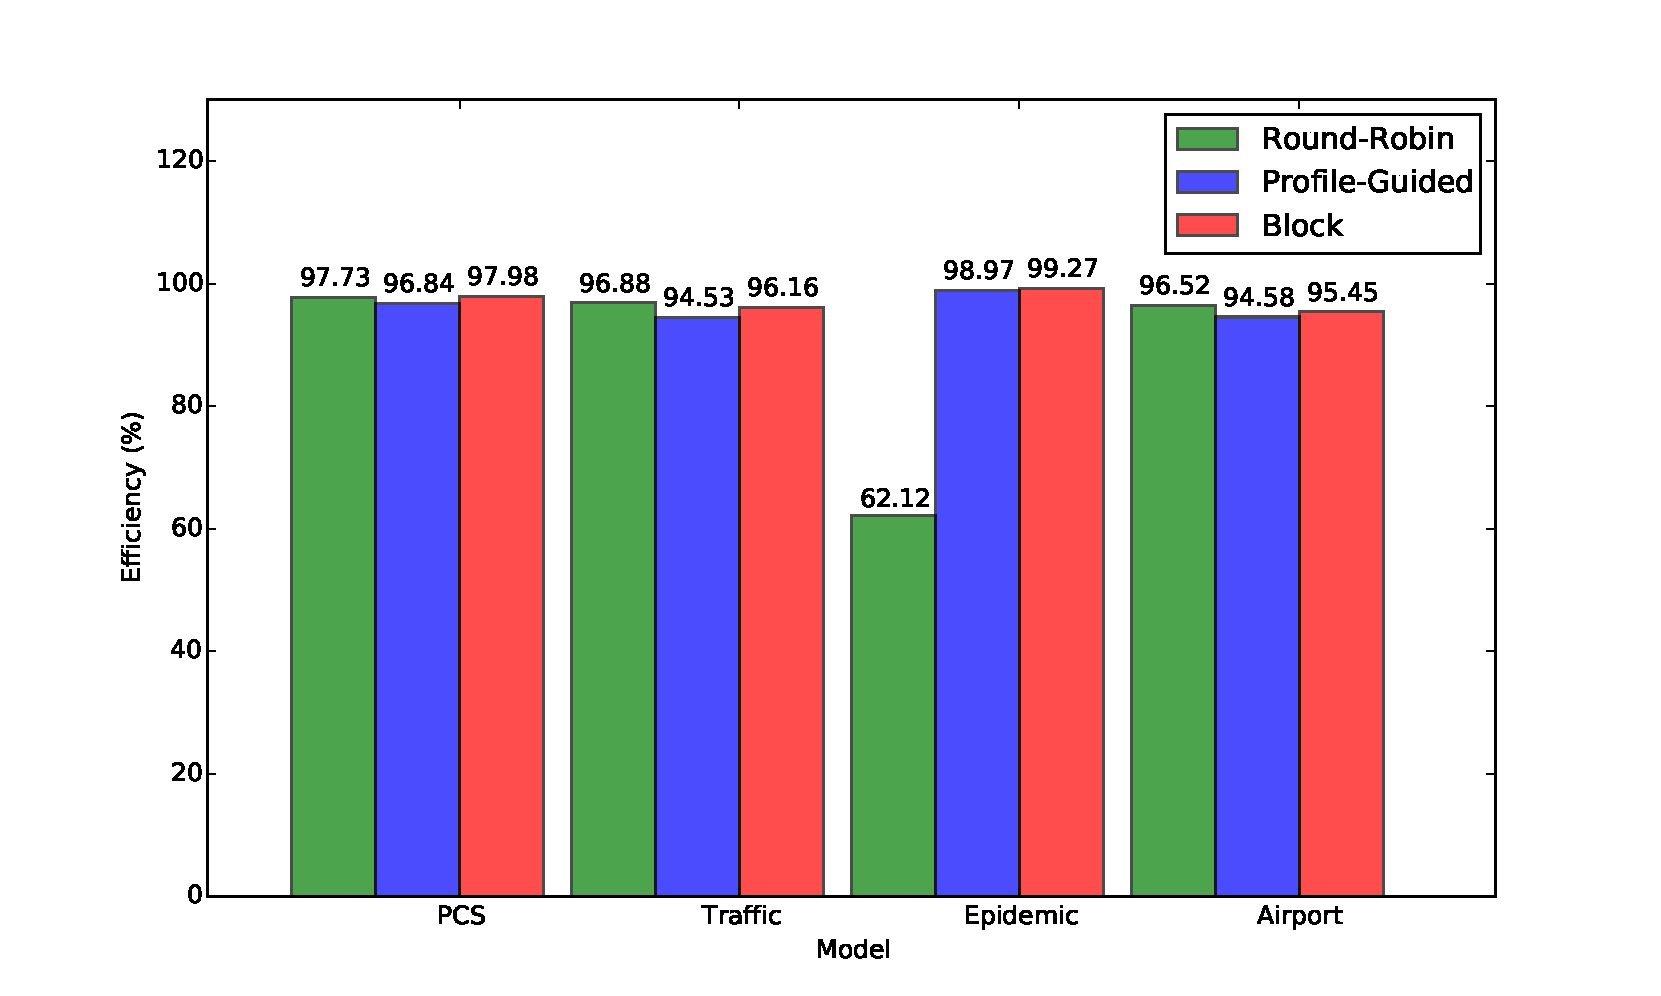
\includegraphics[width=\textwidth,keepaspectratio,quiet]{figs/partitioning_communication/partitioning_efficiency_1node.pdf} \\
      Efficiency \\
    \end{center}
  \end{minipage}
  \caption{LTSF Partitioning: Intel\textsuperscript{\textregistered} Xeon\textsuperscript{\textregistered} E5410 Processor}
  \label{ltsf_partitioning_beowulf}
\end{figure}

\begin{figure}
  \begin{minipage}{.5\textwidth}
    \begin{center}
      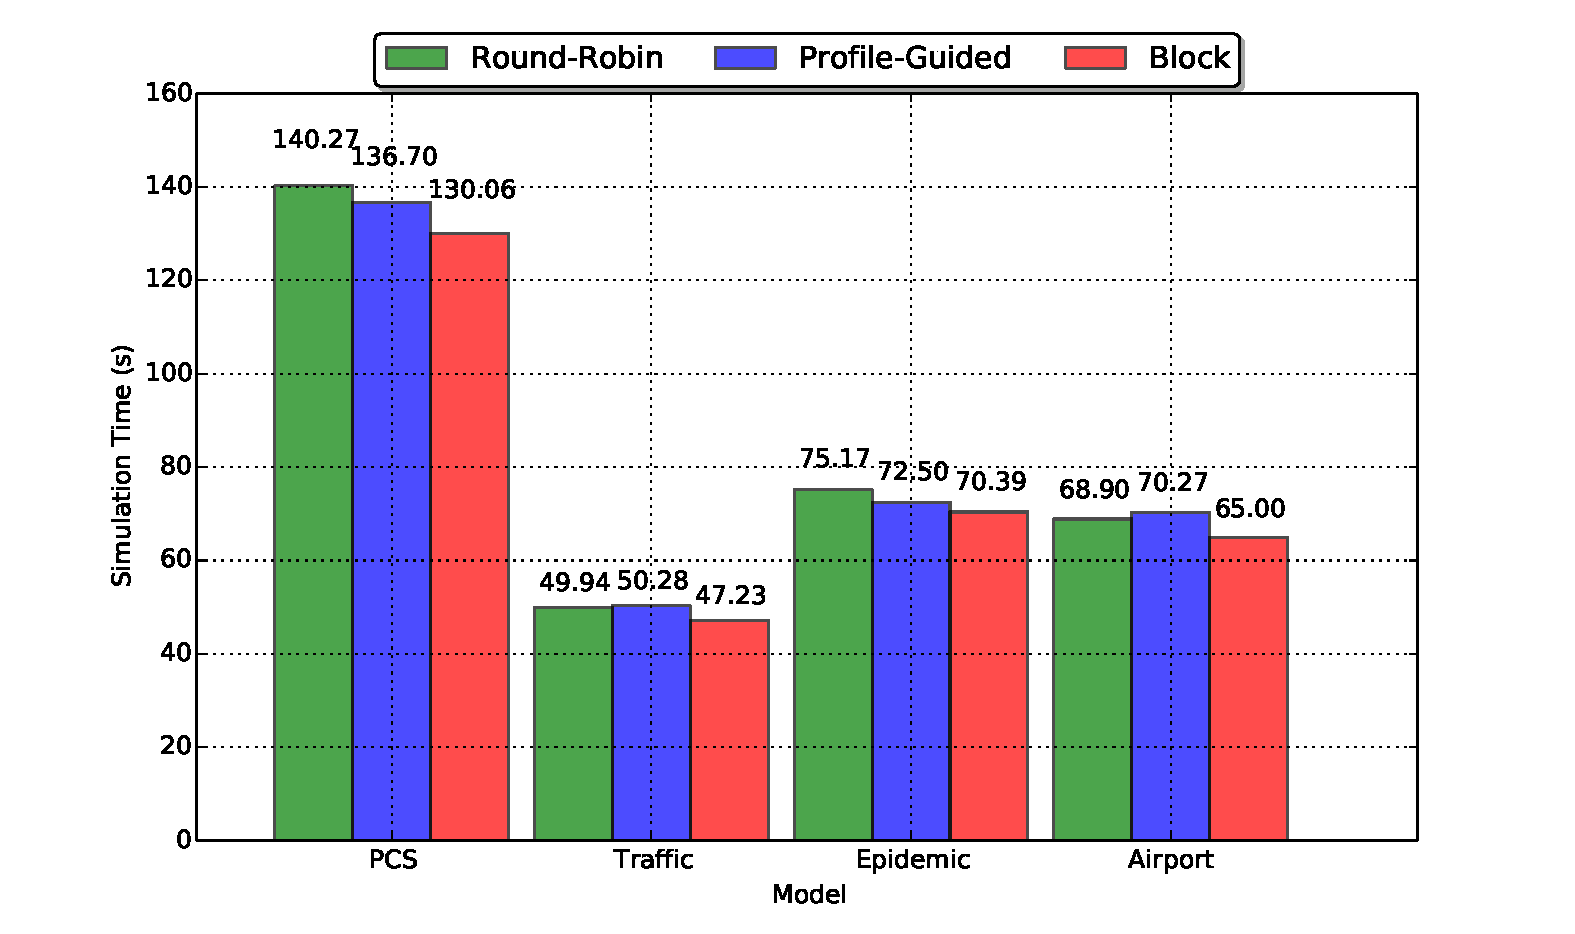
\includegraphics[width=\textwidth,keepaspectratio,quiet]{figs/pending_event_set/partitioning_time.pdf} \\
      Simulation Times (s) \\
    \end{center}
  \end{minipage}%
  \hfill
  \begin{minipage}{.5\textwidth}
    \begin{center}
      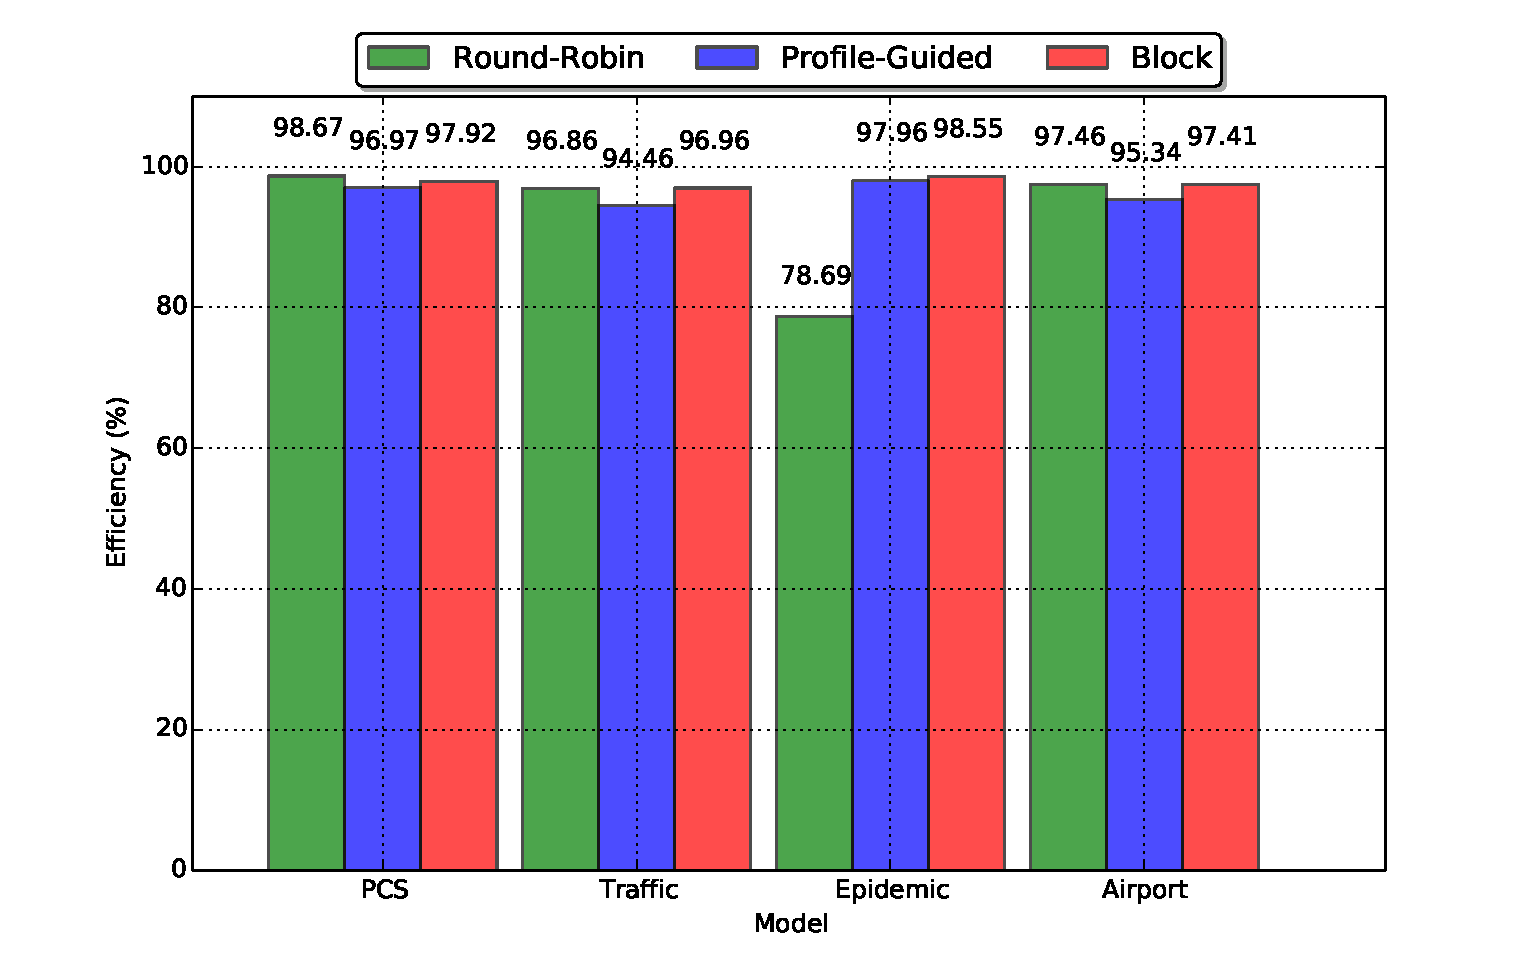
\includegraphics[width=\textwidth,keepaspectratio,quiet]{figs/pending_event_set/partitioning_efficiency.pdf} \\
      Efficiency \\
    \end{center}
  \end{minipage}
  \caption{LTSF Partitioning: Intel\textsuperscript{\textregistered} Xeon\textsuperscript{\textregistered} X5675 processor}
  \label{ltsf_partitioning_bc}
\end{figure}

Just as with the interprocess partitioning, the block partitioning scheme tends to give the best
average performance.  However, only the epidemic model has any significant difference in average
efficiency.  This can be explained by noting that the epidemic model has a very slow event rate
compared to any other model so the efficiency is easy to diminish when the number of rollbacks
increase.

Another interesting observation is that the round-robin partitioning is much worse on the
Intel\textsuperscript{\textregistered} Xeon\textsuperscript{\textregistered} E5410 for the PCS,
traffic, and airport models but not on the Intel\textsuperscript{\textregistered}
Xeon\textsuperscript{\textregistered} X5675.  This, however, is simply a matter of the simulation
model properties, and configurations of the model and kernel.  The LPs of these models are connected
as a grid of 100 x 100 LPs.  Since the number of LTSF queues is a factor of the grid dimensions, the
round-robin partitioning will still provide north-south locality.  The same is not true with 8 LTSF
queues so the simulations will be more unbalanced.

\subsection{State Saving Period}

Instead of saving the state of the LPs after every processed event processed, \textsc{warped2}
allows the user to choose a state saving period value, $N$, so that each LP only has its state saved
every $N$ events.  A larger value of $N$ reduces the amount of time taken to copy states and thus
speeds up forward computation.  The downside is that it also increases rollback time since not all
states are available to roll back to, making it necessary to process more events to get to the
necessary state in a process known as \emph{coast forwarding}.  The total time spent rolling back,
however, is small compared to the time taken for forward computation for moderate values of $N$.

Figure \ref{ssp_analysis_smp_performance} shows the event rates and average number of coast
forwarded events per rollback as the state saving period is increased for all models on a single SMP
machine.  The coast forward rate and rollback rate are also used to analyze state saving and are
related by:

$$ {Coast Forward Rate} = {Coast Forward Events \over Rollbacks} * {Rollback Rate}$$

\begin{figure}
  \begin{minipage}{.5\textwidth}
    \begin{center}
      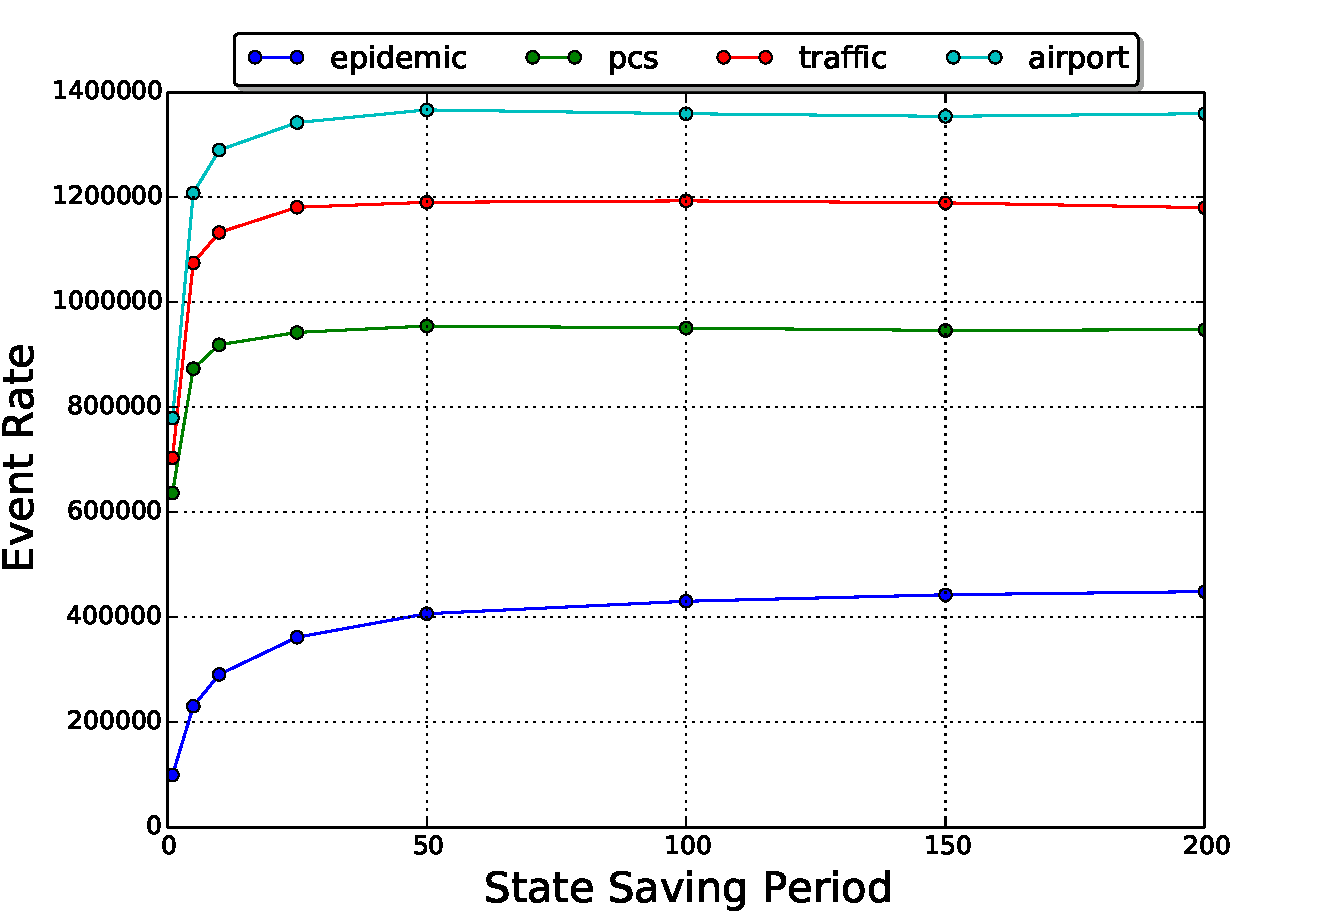
\includegraphics[width=\textwidth,keepaspectratio,quiet]{figs/state_saving/bc/eventrate.pdf} \\
      Event Rate \\
    \end{center}
  \end{minipage}%
  \hfill
  \begin{minipage}{.5\textwidth}
    \begin{center}
      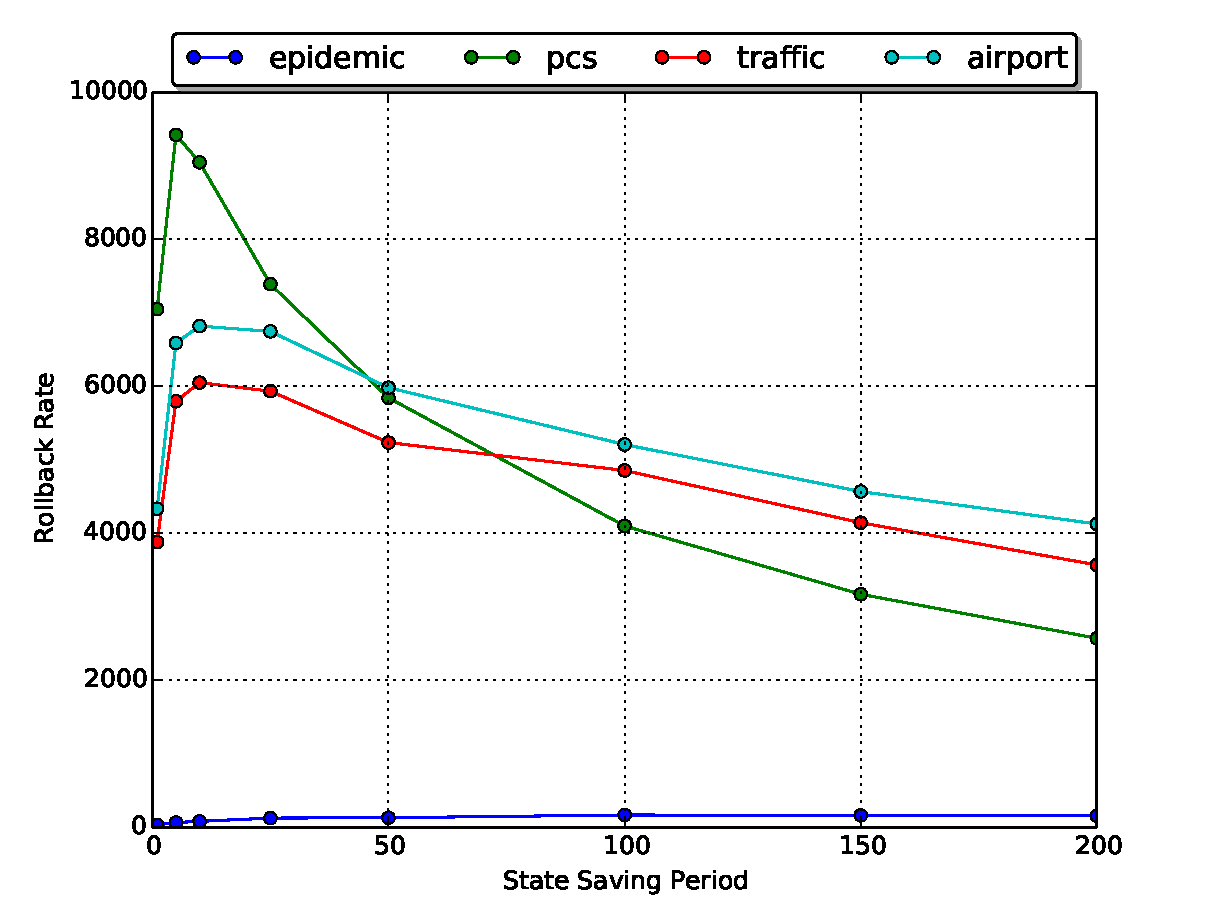
\includegraphics[width=\textwidth,keepaspectratio,quiet]{figs/state_saving/bc/rb_rate.pdf} \\
      $Rollback Rate$ \\
    \end{center}
  \end{minipage}
  \begin{minipage}{.5\textwidth}
    \begin{center}
    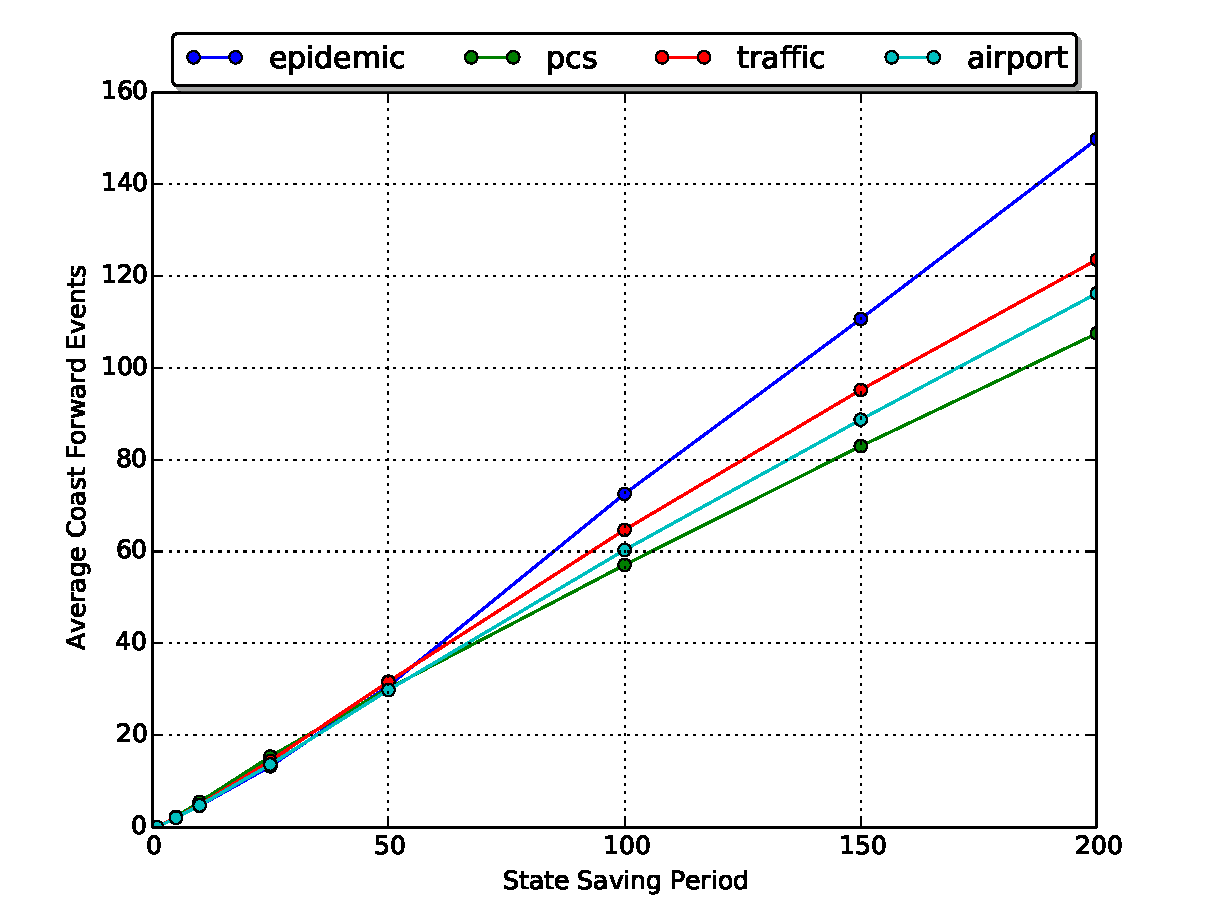
\includegraphics[width=\textwidth,keepaspectratio,quiet]{figs/state_saving/bc/average_cf.pdf} \\
    ${Coast Forward Events \over Rollbacks}$
    \end{center}
  \end{minipage}%
  \hfill
  \begin{minipage}{.5\textwidth}
    \begin{center}
    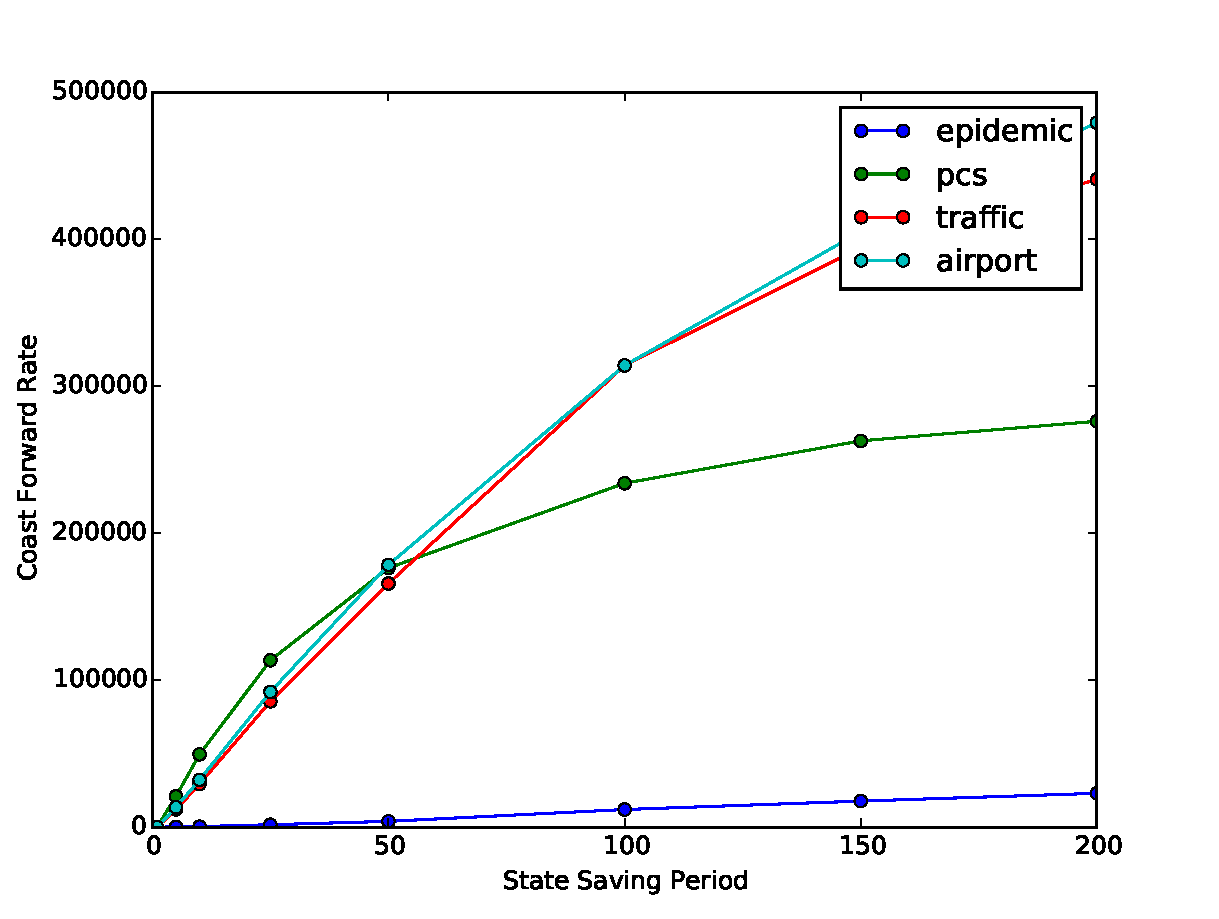
\includegraphics[width=\textwidth,keepaspectratio,quiet]{figs/state_saving/bc/cf_rate.pdf} \\
    $Coast Forward Rate$
    \end{center}
  \end{minipage}
  \caption{Periodic State Saving: Performance on SMP Machine}\label{ssp_analysis_smp_performance}
\end{figure}

For a single SMP machine, the speedup increases significantly for low state saving periods and
flattens out pretty quickly.  The initial speedup is a result of decreasing forward computation time
by removing extra copying.  As the state saving period increases though, the coast forward increases
to the point where it will cancel out the gains time from reduced copying.  An interesting result is
that even though the rollback rate increases for lower state saving periods, a speedup is still
observed.  The coast forwarded rate depends on both the rollback rate and the average number of
events coast forwarded per rollback.  The rollback rate decays exponentially but the average number
of coast forward events per rollback increases linearly.  Therefore the coast forward rate still
increases logarithmically as the state saving period increases since the average number of events
coast forwarded per rollback grows at faster rate than the rollback rate decreases.  Similar results
can be seen in Figure \ref{ssp_analysis_cluster} for a cluster.

\begin{figure}
  \begin{minipage}{.5\textwidth}
    \begin{center}
      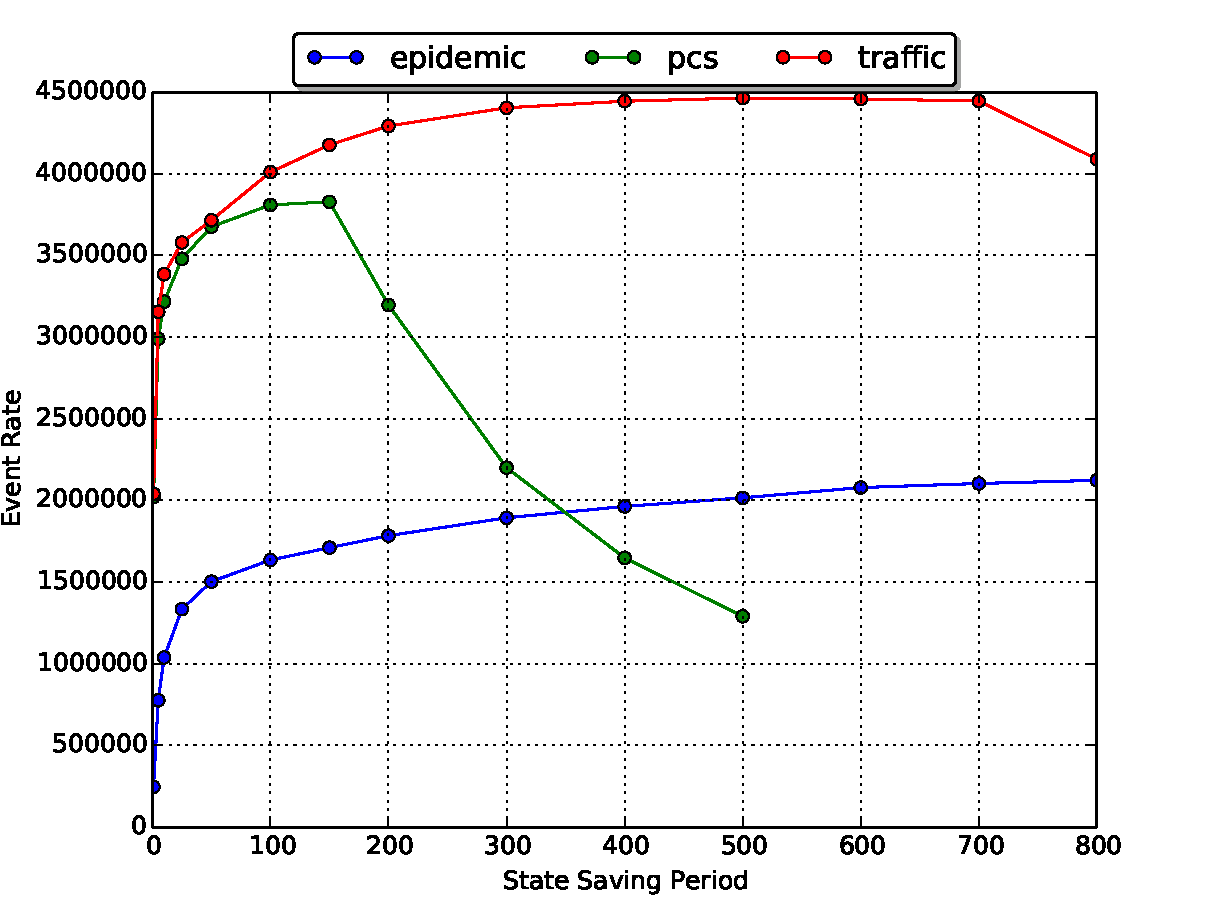
\includegraphics[width=\textwidth,keepaspectratio,quiet]{figs/state_saving/beowulf/eventrate.pdf} \\
      Event Rate \\
    \end{center}
  \end{minipage}%
  \hfill
  \begin{minipage}{.5\textwidth}
    \begin{center}
      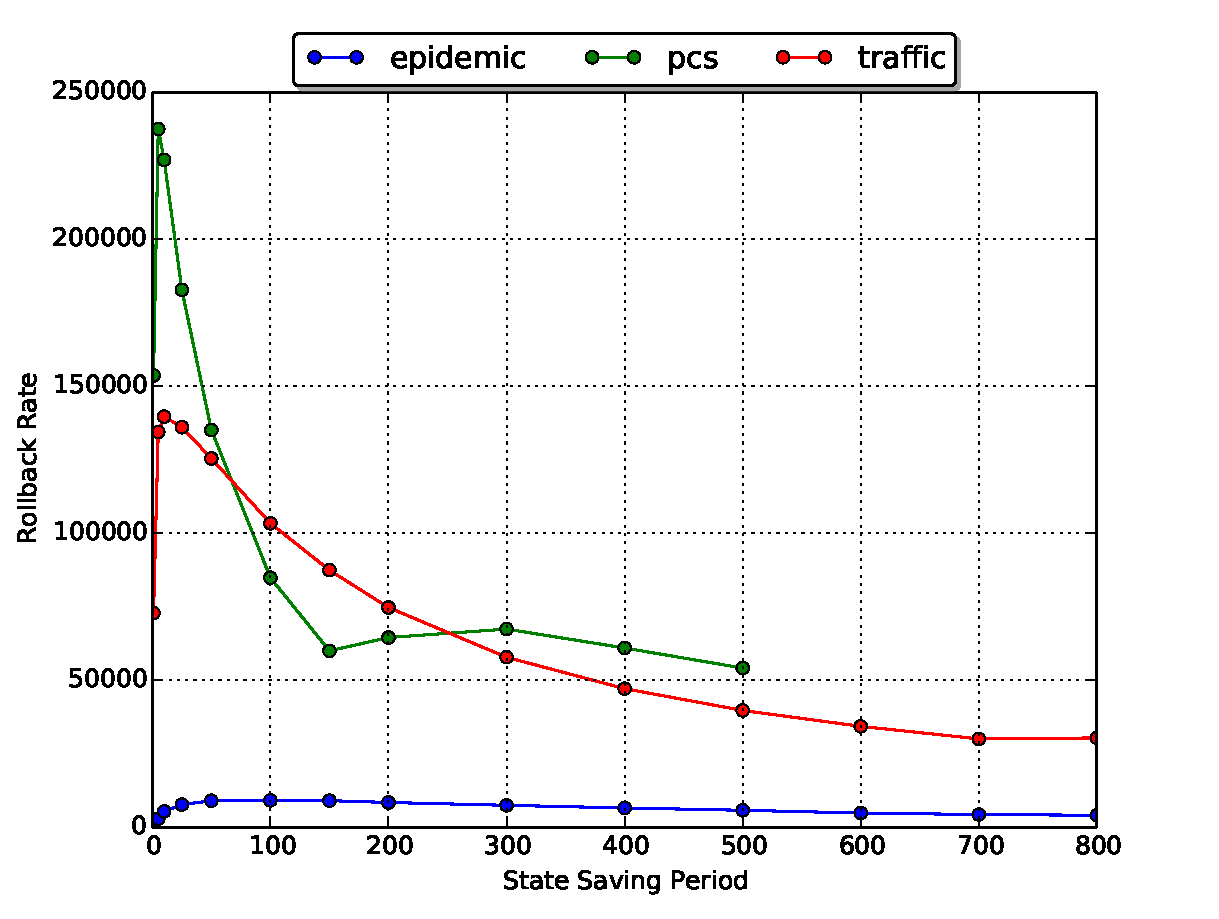
\includegraphics[width=\textwidth,keepaspectratio,quiet]{figs/state_saving/beowulf/rb_rate.pdf} \\
      $Rollback Rate$ \\
    \end{center}
  \end{minipage}
  \begin{minipage}{.5\textwidth}
    \begin{center}
    \includegraphics[width=\textwidth,keepaspectratio,quiet]{figs/state_saving/beowulf/average_cf.pdf} \\
    ${Coast Forward Events \over Rollbacks}$
    \end{center}
  \end{minipage}%
  \hfill
  \begin{minipage}{.5\textwidth}
    \begin{center}
    \includegraphics[width=\textwidth,keepaspectratio,quiet]{figs/state_saving/beowulf/cf_rate.pdf} \\
    $Coast Forward Rate$
    \end{center}
  \end{minipage}
  \caption{Periodic State Saving: Performance on Cluster}\label{ssp_analysis_cluster}
\end{figure}

There are few key observations that become apparent on a cluster that are not seen on a single SMP
machine.  The most apparent is that once the state saving period is increased large enough, a
noticeable jump in the rollback rate starts degrading performance.  This is easily explained by
looking at the magnitude of the rollback rates and coast forward rate for a cluster versus a single
SMP machine.  The cluster has a much larger coast forward rate due to an increased rollback rate
which is a result of an increased discrepancy in communication latency and event processing time.

\section{Protecting Access to LTSF Queues}

Worker threads must be able to access shared data structures without the possibility of race
conditions.  To deal with this, \textsc{warped2} uses mutexes to serialize worker thread access to
any section of code that accesses the LTSF queue.  This method, however can significantly slow down
access to the LTSF queues.  In the default configuration, blocking mutexes are used which means that
if a thread cannot acquire the lock, it will be put to sleep and rescheduled for execution at a
later time.  Blocking mutexes method can waist a lot of extra time if access to the critical section
is quicker than putting the thread to sleep and waking it up again.  All of the accesses to the LTSF
queues are quick in \textsc{warped2} so the locks should only held for a short period of time.

A \emph{spinlock} is a type of mutex that does not force threads to be rescheduled but
instead continue to attempt to aqcuire the lock over and over until it successfully acquires
the lock or the time slice of the thread expires.  The downside of spinlocks is that the CPU time
can be wasted, especially as the number of contending threads increase.  Furthermore, if the
number of total threads is larger than the number of available processors, spinlocks are
even worse because a thread can be involuntarily pre-empted while holding the lock and entire
time slices can be wasted.

\subsection{Spinlocks in \textsc{warped2}}

\textsc{warped2} allows the user to optionally build the kernel to use spinlocks instead of blocking
mutexes.  It is not set as the default because spinlocks do not work well in all cases such as with
a system that is running more threads than processors.  There are many ways to implement spinlocks
with all varying attributes and complexities.  Ticket locks were chosen for \textsc{warped2} because
they are simple to implement, provide fairness to all threads, and generally have good performance
for a small number of threads \cite{lockless-10}.  A short psuedocode algorithm to illustrate the
ticket lock acquisition and release procedures is shown below in algorithm \ref{ticket_lock}.

\begin{algorithm}
\DontPrintSemicolon
\SetKwFunction{fetchAndIncrement}{fetchAndIncrement}
\SetKwBlock{Acquire}{lock}{end}
\SetKwBlock{Release}{unlock}{end}

    \Acquire{
        $my\_number \gets \fetchAndIncrement{next\_number}$\;
        \lRepeat{$ticket = my\_number$}{}\;
    }\;

    \Release{
        $\fetchAndIncrement{ticket}$
    }

    \caption{Ticket Lock Procedures\cite{wiki:ticketlock-15}}\label{ticket_lock}
\end{algorithm}

To acquire the lock, each thread atomically increments a counter and takes the old value as a
``ticket'' to provide FIFO ordering.  Then when the central ticket count reaches the ticket number
of the waiting thread, access to the critical section is given.  To release the lock, the thread
simply increments the central ticket counter and allows the next thread to access the critical
section.  If there is no contention for the lock, the next number will be equal to the ticket number
and a thread can access the critical section immediately.

All previous experiments were run with the default blocking mutexes in which threads will yield the
processor when a lock is contended.  To reduce the average lock acquisition latency, the kernel can
be configured with spinlocks instead.  Figure \ref{spinlock_speedup} shows the speedup for all
models and varying number of LTSF queues.  As expected, the speedup is much greater with more
contention when there are more worker threads per LTSF queue.  It can also be seen that all models
except for epidemic have very similar speedups.  This is probably due to the high cost of saving
such a large complex state.  Contention becomes less of a concern if the event processing is slowed
down by other computation.

\begin{figure}
\centering
  \includegraphics[width=0.5\textwidth,quiet]{figs/pending_event_set/spinlock_speedup.pdf}
  \caption{Speedup with Spinlocks}\label{spinlock_speedup}
\end{figure}



\chapter{GVT and Termination Detection}\label{gvt_termination}

Algorithms that compute the Global Virtual Time (GVT) and detect termination conditions are both
examples of algorithms that can be solved by determining the global state of a distributed system
\cite{chandy-85,lai-87,mattern-89}.  The global state of a system is defined as the combination of
all the local states of the processes in the system and all messages in transit.  Global state
determination algorithms are also commonly used for deadlock detection, garbage collection,
debugging, and checkpointing for failure recovery in distributed systems.

\section{Global Snapshots}

\paragraph{Chandy and Lamport} \cite{chandy-85} described a basic global state algorithm by using
\emph{global snapshots} for distributed systems that use only FIFO channels for communication.  To
start the algorithm, an initiator process records its state and sends a control token out of all
outgoing channels.  When a process receives a control token, and it has not yet recorded its state,
the process records its state and sends more control tokens out of all its outgoing channels.  The
algorithm terminates at each process when it has received a token through all of its incoming
channels.

\paragraph{Lai and Yang} \cite{lai-87} describe an algorithm for non-FIFO systems that computes a
consistent cut by piggybacking a control bit onto basic messages.  The control bit is used to
indicate whether or not the sending process has recorded its state.  The processes can be explained
in terms of colors.  A process that has not recorded its state is colored white and a process that
has recorded its state is red.  White processes send white messages and red processes send red
messages.  The control bit in the messages indicates the color.  All processes are initially white
and turn red when a red message arrives.  When a red message arrives at a white process, the process
must record its state BEFORE actually receiving the message.  The snapshot only relies on basic
messages and no control tokens are used.  This algorithm has several drawbacks.  First, it assumes
that every process will eventually receive a red message and record its state which is not
guaranteed.  Second, to ensure transient messages are recorded, the processes must record all
incoming and outgoing messages and send them to other processes within the basic messages.  That way
the transient messages can be calculated by differences in incoming and outgoing messages.

\paragraph{Mattern} \cite{mattern-93} extended the algorithm by Lai and Yang by adding a separate
control token which is used to create two cuts by circulating the control token to every process
twice.  The control token is used to color the processes instead of the basic messages.  This
guarantees that every process will eventually record its state because the token is always
circulated.  Furthermore, processes do not have to keep track of sent and received messages.
Instead counters can be used to keep track of the differences in sent and received white messages at
each process.  The control token can then accumulate the counts.  When the white message counts
accumulate to zero when the token arrives back at the initiator process, it can be determined that
the snapshot is complete.  These counters can be \emph{vector counters} or \emph{scalar counters}.
Vector counters keep track of messages to/from each process individually whereas scalar counters
keep track of just a single count at each process.  When the algorithm is complete, only the
initiator process can produce a global snapshot so if all processes must use the snapshot, it must
be broadcast to the other processes.

\section{GVT}

Although GVT algorithms can be implemented with the basic global snapshot algorithms described
above, it is usually more efficient to build custom solutions on top of the basic algorithms.  In a
GVT algorithm, the local minimum clock of process is the local state and the basic messages are
events that are sent between processes.  This section first describes the key ideas that must be
considered when developing a GVT algorithm.  Then, a few of the classic GVT algorithms and modern
GVT algorithms that are commonly used in practice today are described.  Finally, the algorithm that
is implemented in \textsc{warped2} is described as well as the reasons for choosing the approach.

GVT algorithms can be synchronous or asynchronous.  In a synchronous GVT algorithm, since all other
computation will be blocked, event processing will be halted.  Synchronous GVT algorithms are
usually very simple to implement but halting the event processing can be costly.  On the other hand,
asynchronous GVT algorithms calculate GVT concurrently with event processing.  For this reason,
asynchronous GVT algorithms perform much better than synchronous GVT algorithms but are harder to
implement because special cases must be considered.

There are two special cases that must be considered in a GVT algorithms:

\begin{description}
    \item[Transient Message Problem:] is caused by messages(events) that have been sent by the
      sending process but not yet received by the receiving process.  If not carefully considered in
      a GVT algorithm, these \emph{transient messages} can be completely missed which could lead to
      an erroneous GVT calculation if they contain the minimum timestamp of all other events in the
      system.
    \item[Simultaneous Reporting Problem:] is caused because processes can report their local
      minimum clock at different points in real time.  Consideration must be taken into account to
      ensure that a process does not report its local minimum clock value and then receive an event
      from a process that has not yet reported its local minimum clock value, completely missing the
      event.
\end{description}

\noindent
There are many synchronous and asynchronous GVT algorithms that have been developed over the years
that all have some method of either solving these problems.

\subsection{Asynchronous GVT Algorithms}

\subsubsection{Message Passing Algorithms}

Most of the Time Warp systems in use today are based on message passing and classically GVT
algorithms have been designed for message passing systems.  In this section Samadi's and Mattern's
message passing algorithms \cite{samadi-85, mattern-93} are discussed and in the next section
Fujimoto's shared memory GVT algorithm \cite{fujimoto-94} is discussed as well as the Seven O'Clock
algorithm \cite{bauer-05} which is an extension of Fujimoto's shared memory algorithm extended
for distributed memory systems.

\paragraph{Samadi's Algorithm}\cite{samadi-85} in the most general form uses acknowledgements for
all events that have been received.  All processes must track all events that have been sent but
have not been acknowledged.  Furthermore, the received messages must also be tracked so that
acknowledgements can be sent.  All transient message can then be calculated from the tracked
messages.  A process initiates the GVT algorithm by broadcasting a start message to all processes.
After this start message is received by a process, it is marked(colored) and all acknowledgements
sent from a marked process are also marked(colored).  All processes then calculate their local
minimum by taking the minimum of the unacknowledged received events, the marked acknowledgments
sent, and the local simulation clock.  Marking the acknowledgements sent after the start of the GVT
calculation ensures that the simultaneous reporting problem will not occur.

\paragraph{Mattern's Algorithm} \cite{mattern-93} for GVT calculation is an extension on his general
snapshot algorithm that was described above.  The white message counts are used to determine whether
transient messages are still in the system.  They also serve as the basis for determining when the
snapshot is complete which occurs when the accumulated white message count of all processes is zero.
To ensure that the simultaneous reporting problem does not occur, red messages sent are recorded and
used in the local minimum value of the sending process.  The algorithm is initiated by sending a
control token to all processes in some defined order.  The token accumulates the white message
counters, local minimum clocks, and minimum red message timestamps.  When the accumulated count
reaches zero and the token is back at the initiator process, the GVT is approximated using the
minimum of the accumulated clocks and red message timestamps.

\subsubsection{Shared Memory Algorithms}

\paragraph{Fujimoto's Algorithm} \cite{fujimoto-94} is a fast GVT algorithm that exploits properties
of shared memory architectures.  In most shared memory architectures, processors cannot observe
memory operations in different orders.  For this reason, it is not possible to have transient
messages if a shared data structure is used to communicate between tasks running on different
processors.  Furthermore, a shared flag variable can be used to initiate the GVT algorithm.
However, it is still possible that the flag can be read at different times, so the simultaneous
reporting problem can still occur.  To solve the simultaneous reporting problem, two things must be
done. First, the start flag is checked after sending events and recorded if the sending task has not
yet reported its local minimum value and is eventually used when the reporting is done.  Second, the
start flag must be read into a temporary local variable before obtaining a new event to process.

\paragraph{Seven O'Clock Algorithm} \cite{bauer-05} is an extension of Fujimoto's algorithm for
distributed memory systems.  Although the algorithm can be used in message passing systems, the
algorithm does not require any messages and is still uses shared memory ideas.  The key idea in the
algorithm is that all processors in a distributed system all have a consistent view of wall clock time.
Hence, the processors can carry out an operation in an atomic manner without having to explicitly
interact.  The atomicity can be achieved by using cycle level counters which are available on most
modern architectures.  Unlike Fujimoto's algorithm though, transient messages can still be missed in
the calculation.  To solve that problem, each processor must wait a small time interval which is
calculated based on the worst round trip time for network transactions.

\subsection{Synchronous GVT Algorithms}

\paragraph{Global Reductions} provide a good way to do a synchronous minimum calculation which and
is a common way to implement a synchronous GVT algorithm.  ROSS implements a synchronous GVT
algorithm which uses global reductions to implement a variant of Mattern's algorithm\cite{holder-08}.
First, to prevent the transient message problem, a global reduction on
message counts of each process is performed until the total reaches zero.  Any events received after
the start of the algorithm are recorded and included with the local minimum of the receiving
process.  When the messages count reaches zero a global reduction is performed on the local minimum
timestamp of all processes which yields a GVT value for all processes.  This algorithm is efficient
when Time Warp simulation are run on large supercomputing platforms like the blue gene machine which
perform collective operations very quickly.

\subsection{GVT in \textsc{warped2}}

\textsc{warped2} implements both synchronous and asynchronous GVT algorithms.  For the asynchronous
GVT algorithm, Fujimoto's shared memory algorithm is used between worker threads and a variation of
Mattern's algorithm with scalar message counters is used between processes.  The synchronous
algorithm is based on the global reduction algorithm mentioned above but also includes a reduction
between worker threads as well as two thread synchronization barriers.

The details of how a GVT algorithm is integrated into the worker threads in \textsc{warped2} is
outlined below in algorithm \ref{gvt_workers} which shows the main event processing loop with an
emphasis on GVT contribution as well as the send routine and the remote event receive routine.  This
system of GVT integration is fairly ambiguous and should work for any combination of shared memory
and message passing GVT algorithms whether they are synchronous or asynchronous.

\begin{algorithm}
\DontPrintSemicolon
\SetKw{Continue}{continue}
\SetKw{In}{in}
\SetKwFunction{GetNextEvent}{getNextEvent}
\SetKwFunction{Report}{reportThreadMin}
\SetKwFunction{ReportSend}{reportThreadSendMin}
\SetKwFunction{ProcessEvent}{processEvent}
\SetKwFunction{SendEvent}{sendEvent}
\SetKwFunction{GVTSendUpdate}{GVTSendEventUpdate}
\SetKwFunction{GVTReceiveUpdate}{GVTReceiveEventUpdate}
\SetKwBlock{Process}{processEvents}{end}
\SetKwBlock{Send}{sendEvent}{end}
\SetKwBlock{Receive}{receiveRemoteEvent}{end}

    \Process{
        \While{termination not detected} {
            $localGVTFlag_i \gets localGVTFlag$

            $e \gets \GetNextEvent{}$\;
            $lp \gets$ receiver of $e$\;

            \If{$localGVTFlag_i$ and ($workerThread_i$ hasn't reported local min)}{
                \Report{$timestamp_e$}\;
            }

            \If{$e$ is straggler}{
                Rollback $lp$\;
                \Continue\;
            }

            $newEvents \gets \ProcessEvent{e}$\;
            
            \ForEach{$ne$ \In $newEvents$}{
                \SendEvent{$ne$}\;
            }
        }
    }\;

    \Receive{
        \GVTReceiveUpdate{$timestamp_e$, $color_e$}\;
        $lp \gets$ receiver of $ne$\;
        Insert into Unprocessed Queue for $lp$\;
    }\;

    \Send{
        \uIf{$ne$ is remote event}{
            $color \gets \GVTSendUpdate{ne}$\;
            Insert into Send Queue\;
        } \Else {
            $lp \gets$ receiver of $ne$\;
            Insert into Unprocessed Queue for $lp$\;
        }

        \If{$localGVTFlag_i$ and ($workerThread_i$ hasn't reported local min)}{
            \ReportSend{$timestamp_ne$}\;
        }
    }

    \caption{GVT: Worker Threads}\label{gvt_workers}
\end{algorithm}

The routines for \texttt{ReportThreadMin}, \texttt{GVTReceiveEventUpdate},
\texttt{GVTSendEventUpdate}, and \texttt{ReportThreadSendMin} are intentionally abstract since they
will vary with the exact GVT algorithm implementation.  In general though, the purpose of each
doesn't really change.  The purpose of each is:

\begin{description}
    \item[ReportThreadMin ] is used for the worker threads to report a minimum event timestamp which
      will usually be the current event since the LTSF queue orders events.
    \item[ReportThreadSendMin ] is used for the worker threads to report any events that are sent
      after the localGVTFlag has been set and it has not yet called \texttt{ReportThreadMin}.
    \item[GVTReceiveEventUpdate ] is used to update any message counters, send acknowledgements or
      record the timestamps of received events.
    \item[GVTSendEventUpdate ] is used to update any message counters, track sent messages, or get
      the current color of the process to tag events being sent.
\end{description}

\noindent
This system of GVT calculation will work as long as the localGVTFlag indicator is retrieved before
obtaining the next event and the sends are reported after sending an event.  The manager thread
controls the initiation and termination of the GVT algorithms and will vary greatly depending
on the exact implementation.

\subsubsection{Asynchronous}

The asynchronous GVT algorithm in \textsc{warped2} is based around a variant of Mattern's algorithm
\cite{mattern-93} for the message passing part.  In the \textsc{warped2} implementation, scalar
counters are used to keep track of whites message instead of vector counters.  That means that each
process keeps track of the number of sent messages minus the number of received messages to and from
all other process as a single count.  The reason that scalar counters are used over vector counters
is that vector counters require extra space and are only necessary if communication is stopped after
receiving a control token until all known transient messages that are bound for the receiving
process are received.  With scalar counters, this is not possible because all counts are combined
into a single counter.  However, with scalar counters it is possible that more than two rounds of
the control token will be necessary.  This is usually not a problem in practice though since two
rounds is usually sufficient.  Also, each process must maintain a counter for both white messages
\emph{and} red messages so that counters can be consistent between multiple runs of the algorithm.
The roles of the colors must also be switched between successive runs.

Another major different between the classic Mattern algorithm and the variant in \textsc{warped2} is
that the classic algorithm assumes that the timestamps of the white messages that are received will
be processed right away and counted in the minimum clock value when a token is received.  Since this
is not the general case in \textsc{warped2}, a running minimum of the white message timestamps
received is recorded and included in the minimum clock value when a token is sent to ensure that all
white messages are included in the final GVT value.

A GVT token will be sent by the manager thread when the local GVT calculation based on Fujimoto's
shared memory algorithm \cite{fujimoto-94} is completed.  The local GVT calculation will begin
either when a token is received or when the initiator process determines that is should start.  The
initiator process is the process with PID of 0 and the start of a new calculation is some fixed time
interval from the start of the previous calculation.

The asynchronous algorithm described above works well in cases where the remote communication is
relatively low but has been shown to be problematic under heavy remote communication.  The root of
the problem is that the GVT token must compete with remote events that must be sent and received.
Based on some observations that show large message counts, the bigger problem with being able to
complete receives quickly.  To get around this constraint, users can either increase the number LPs
or decrease the number of worker threads to reduce the network load.

\subsubsection{Synchronous}

The synchronous GVT algorithm is a simple extension of the reduction algorithm implemented in the
ROSS simulation kernel.  The biggest difference is that the manager thread must block the worker
threads from processing any more events.  Also, unlike the algorithm used in ROSS, the processes are
explicitly colored so that any events that are inserted into the remote send queue after the GVT
calculation is started are known to be included with the sending process's local minimum value.  The
algorithm executed by the manager thread is summarized in the pseudocode in Algorithm
\ref{gvt_manager_synchronous}.

\begin{algorithm}
\DontPrintSemicolon
\SetKw{Break}{break}
\SetKwFunction{SumAllreduce}{sumAllreduce}
\SetKwFunction{MinAllreduce}{minAllreduce}
\SetKwBlock{ProgressGVTs}{progressGVT}{end}

    \ProgressGVTs{
        $color \gets RED$\;
        $localGVTFlag \gets 1$\;
        $THREAD\_SYNCHRONIZATION\_BARRIER$\;\;

        \While{$true$}{
            Flush send queue\;
            Receive messages\;
            $\SumAllreduce{localMsgCount, globalMsgCount}$\;
            \lIf{$globalMsgCount = 0$}{\Break}
        }\;

        $localMin \gets recvMin$\;
        \ForEach{worker thread, i}{
            $localMin \gets \min{(localMin, \min{(localMin_i, sendMin_i)})}$\;
        }\;

        $\MinAllreduce{localMin, GVT}$\;\;

        $color \gets WHITE$\;
        $localGVTFlag \gets 0$\;
        $THREAD\_SYNCHRONIZATION\_BARRIER$\;
    }

    \caption{Synchronous GVT: Manager Thread}\label{gvt_manager_synchronous}
\end{algorithm}

When the worker threads report their local minimum, they must wait at \emph{two} thread barriers.
Both barriers are needed so that the manager thread can ensure that no more remote events are sent.
When every worker thread calls the first barrier, it indicates to the manager thread that it all
local minimums have been reported and it can continue.  The second barrier is an indicator to the
worker threads so they can be released and continue processing events.

The advantage of the synchronous GVT algorithm in \textsc{warped2} is that it is very robust and
works well even under very heavy remote communication.  Furthermore, it will be produce the exact
GVT unlike the asynchronous algorithm since event processing will not continue until it is complete
so the GVT cannot increase.

\section{Termination Detection}

Termination detection, like GVT, is a problem of determining the global state of the system.
Termination is a \emph{stable property} of a distributed system, meaning that once termination
conditions occur, the system will remain with termination conditions forever until further action is
taken.

A process in the system can be in one of two states at any time: \emph{active} or \emph{passive}.  A
process is considered active if some basic computation still remains and passive otherwise.  When
all processes in the system become passive and no messages are left in transit, then the system
should be terminated.  The purpose of the termination detection algorithm is to determine when this
occurs.  A passive process can become active with the arrival of an \emph{activation message}.  For
parallel discrete event simulation the basic computation is event processing and the activation
messages are events.  A termination detection algorithm for any parallel discrete event simulation
must satisfy the following properties:

\begin{description}
    \item[Safety Property:] Termination will not be detected if any unprocessed event is still
      present in system which includes all unprocessed events that have been received at each
      process and events still in transit.
    \item[Liveness Property:] Termination will be detected at some finite amount of time after all
      events have been processed.
\end{description}

\noindent
Just like GVT algorithms, termination detection algorithms can implemented with message passing or
shared memory communication.  Termination algorithms vary widely because different systems can
define termination conditions in such different ways.  Furthermore, termination usually does not
affect system performance as long it does not block event processing so correctness is more
important than optimization.  The rest of this section will only focus on the algorithms that are
implemented in \textsc{warped2}.

\subsection{Termination in \textsc{warped2}}

The termination detection algorithm in \textsc{warped2} is actually two independent algorithms, a
message passing algorithm and a shared memory algorithm, merged into a single algorithm.  In
contrast to the GVT algorithm, the shared memory algorithm is actually used to initiate the message
passing algorithm.

\subsubsection{Shared Memory algorithm}

The purpose of the shared memory algorithm is to determine when all of the worker threads in a
process become passive (inactive).  The algorithm is fairly straightforward and uses just a shared
counter variable to keep track of the number of active worker threads and a array to keep track of
the state of each worker thread.  Each worker thread updates their own state when they change and
atomically update the counter.  The manager thread periodically checks to see if the counter has
reached zero.  If the count has reached zero and the process is the master, then the interprocess
message passing algorithm is initiated.  The integration of the shared memory algorithm is
illustrated in algorithm \ref{termination_workers}.  To allow the GVT calculation to continue,
worker threads in a passive state must still report an infinite local minimum value.

\begin{algorithm}
\DontPrintSemicolon
\SetKw{Continue}{continue}
\SetKw{In}{in}
\SetKwFunction{Report}{ReportThreadMin}
\SetKwFunction{GetNextEvent}{getNextEvent}
\SetKwFunction{ProcessEvent}{processEvent}
\SetKwFunction{SendEvent}{sendEvent}
\SetKwBlock{Process}{processEvents}{end}
\SetKwBlock{Send}{sendEvent}{end}

    \Process{
        \While{termination not detected} {
            $localGVTFlag_i \gets localGVTFlag$\;
            $e \gets \GetNextEvent{}$\;
            \If{$e \neq nullEvent$} {
                \If{$state_i = PASSIVE$}{
                    $state_i = ACTIVE$\;
                    $activeCount \gets activeCount + 1$\;
                }
                \;
                $lp \gets$ receiver of $e$\;
                \If{$e$ is straggler}{
                    Rollback $lp$\;
                    \Continue\;
                }
                \;
                process event $e$\;
                send new events\;
            } \Else {
                \If{$state_i = ACTIVE$}{
                    $state_i = PASSIVE$\;
                    $activeCount \gets activeCount - 1$\;
                }
                \If{$localGVTFlag_i$ and ($workerThread_i$ hasn't reported local min)}{
                    \Report{$\infty$}\;
                }
            }
        }
    }
    \caption{Termination: Worker Threads}\label{termination_workers}
\end{algorithm}

The safety property is not necessarily achieved with this algorithm because it is possible that the
last active thread sends an event to another LP which will be processed by another thread.  Then if
the sending thread becomes inactive, all threads can be temporarily inactive and the manager thread
can falsely detect termination.  However, it is very unlikely that the sending thread will report
itself as passive before the receiving thread gets the event and reports itself as active.
Furthermore, the manager thread is forced to check the active thread counter at least twice with no
changes in any worker thread state.  The challenge with completely solving this problem is that it
is not known which thread will process the event since LPs are mapped to LTSF queue and not directly
to worker threads.

The liveness property is achieved because the manager thread periodically checks the active
worker thread count so the inactivity of all worker threads will eventually be discovered.

\subsubsection{Message Passing Algorithm}

The algorithm that is carried out among processes is an asynchronous message passing algorithm based
on Mattern's ``sticky flags'' algorithm \cite{mattern-91}.  Similar to the GVT algorithm, the token
is passed in a logical ring to increasing PIDs.  However, the initiator process of the algorithm can
change with each execution of the algorithm.  The initiator of each successive execution is the
first active process that the token reaches during the previous circulation.  For the first
circulation, the initiator is the process with the PID of 0.

Each process has two state indicators, one for the actual state and one for the \emph{sticky state}.
When the sticky state of all processes are simultaneously passive, then the simulation can terminate
safely.  The sticky state becomes active when the actual state becomes active but sticks to active
when the actual state becomes passive.  It can only change to passive on the arrival of a token
which forces the token to circulate two times with no process becoming active and ensures the safety
property.  Without this scheme, a process that has already forwarded the token because it was
passive could receive an activation message and then the sender of the activation message could
become passive before receiving the token and false termination could then be detected.

The algorithm is started when the initiator process becomes passive which is determined by the
shared memory algorithm.  When a process receives the token it becomes the initiator but loses its
roles as initiator when it sends the token.  That way, only a single process can be the initiator.
Furthermore, since the token always stops at an active process, the token is always guaranteed to
start again when it becomes passive which also guarantees the liveness property.  When the token is
received back at the initiator with a passive state, then termination is signaled to all processes.
The procedure is illustrated in Algorithm \ref{termination_token_receive}.

\begin{algorithm}
\DontPrintSemicolon
\SetKw{And}{ and }
\SetKwFunction{SendToken}{SendToken}
    $initiator \gets true$\;
    \If{$state_{sticky} = PASSIVE \And PID = minitiator$} {
        \If{$mstate = PASSIVE$ \And $mcount = 0$} {
            Signal termination\;
        }
    } \ElseIf{$state_{sticky} = PASSIVE$} {
        $initiator \gets false$\;
        \SendToken{$mstate, minitiator, mcount$}\;
    }
    $state_{sticky} \gets state_{actual}$\;
\caption{Termination Token Receive}\label{termination_token_receive}
\end{algorithm}

It should also be noted that this algorithm is only guaranteed to work if the message order is
preserved between any two processes or if it can be determined that no transient messages can exist.
For this reason, the termination algorithm also keeps message counters and accumulates the counters
from each process just like with the Mattern GVT algorithm.



\chapter{Memory Management}\label{memory_management}

This chapter will focus on main topics related to memory management in a Time Warp system and their
implementations in \textsc{warped2}.  The topics will include state saving, fossil collection and
memory allocation \cite{fujimoto-90,fujimoto-00}.  The memory requirements and performance for
different state saving, fossil collection, and memory allocation techniques can vary greatly.

\section{State Saving}

\subsection{State Saving Techniques}

\paragraph{Copy-state Saving} is the classic state saving technique that saves every past state of
every LP and requires that the all states are copied and saved into the state queues.  This method
requires a lot of extra memory and requires a lot of extra computation to copy the states and insert
them into the state queue.  For this reason, copy-state saving is usually used in conjunction with
other technique or not at all.

\paragraph{Periodic State Saving} is another state saving technique where the state of each LP is
saved only once every $N$ events, where $N$ is a number greater than one.  Periodic state saving can
significantly reduce the overhead of the time taken to copy the state of the LPs into the state
queue.  However, due to state history being lost, more processed event have to be saved so that the
state of LPs can be restored correctly.  These saved events must be reprocessed to restore the state
in a process known as \emph{coast forwarding}.  During coast forwarding the events are processed
normally but only to update the state.  The only difference is that no events are sent during the
coast forwarding phase.  The downside is that the rollback length is increased due to the loss in
state saving.  However, periodic state saving is a significant improvement over the base copy-state
staving approach since the reduced time in state saving far outweighs the extra rollback time for
increased rollback length.

\paragraph{Incremental State Saving} is a technique that aims to reduce the amount of memory needed
to store past states of the LPs.  Instead of saving entire snapshots of the past states, the
differences in specific state variables are saved.  This method requires that metadata describing
which variables are modified for each event.  Therefore, this approach works well as long as only a
small portion of the state variables change during the forward execution of events.

\paragraph{Reverse Computation} \cite{carothers-99a} is a modern approach to state state saving that
does not actually save any past states of the LPs.  Instead, the \emph{control state} of the forward
computation is saved as a set of bits that describe the forward control flow.  By saving the control
flow of the forward execution for each event, the state variables that are modified and how they are
modified are known and can be reversed.  This is the case at least if all state variables are
reversible without the need to know the histories of the variables.  Also, a reversible random
number generator is required.  The major problem with this approach is the necessity to understand
forward and reverse computation precisely in the implementation of the simulation model.

\subsection{State Saving in \textsc{warped2}}

\textsc{warped2} currently implements periodic state saving because it is simple to understand and
does not require that model developers know anything about it.  Furthermore, it can increase
performance and decrease memory requirements for any type of simulation model.

\section{Fossil Collection}

When the events and states in the processed queues, output queues, and state queues are no longer
needed, the memory that they consume is no longer needed and can either be freed or reused.  Fossil
collection is the process of reclaiming memory for future use \cite{fujimoto-90,fujimoto-00}.  There
are many methods of fossil collection that have been used in practice.

\subsection{Fossil Collection Techniques}

\paragraph{GVT-based Fossil Collection} is the traditional method of fossil collection.  Since
rollbacks cannot occur past the GVT, it can be used be used as a marker to indicate what can be
fossil collected.  Fossil collection is triggered after every GVT calculation and all memory is
explicitly freed so that it can be reallocated for future use.

\paragraph{On-the-fly Fossil Collection} is a method of fossil collection used in GTW which does not
use GVT as a starting point and memory is not explicitly freed.  Instead, after events are
processed, they are added to one of the per-processor free memory lists.  New events can then be
allocated from a list as long the first event in the list has a timestamp less than the GVT.  If it
does not then the current event being processed is either aborted until the GVT reaches a higher
value or the list is searched for a lower timestamp event.  This approach however, has been shown to
produce instability caused by imbalances in rollbacks which creates imbalances in the free lists,
and ultimately leads to a lot of aborted events or a long search time \cite{carothers-00}.

\paragraph{Optimistic Fossil Collection} \cite{young-98-dsc} is another method of fossil collection
which, like on-the-fly aims to reuse memory instead of explicitly freeing it.  However, optimistic
fossil collection is based on a statistical bound for rollbacks.  It is still possible that memory
that was fossil collected could still be used.  This situation is called an OFC fault.  Therefore,
methods such as global state checkpointing must also be implemented to recover from these faults.

\subsection{Fossil Collection in \textsc{warped2}}

Currently, \textsc{warped2} implements a GVT-based fossil collection.  The GVT is calculated by
the manager thread but there are two ways that fossil collection can be achieved in \textsc{warped2}.
The first way is to have the worker threads fossil collect one LP at a time as they process events.
The last fossil collect time can be recorded for each LP so that the worker threads can know when fossil
collection is needed by comparing the times to the current GVT.  The second way is to have the
manager thread fossil collect all LPs.  Once the GVT is calculated, all LPs can be fossil collected
all at once.

With manager thread fossil collection, the worker threads are relieved from unnecessary work
that can slow down event processing but extra locks will be needed to protect access to the
processed queue, output queue, and state queue for each LP.  Worker thread fossil collection
will be the more scalable approach for both the number of LPs and the number of processes since
the manager thread must perform other tasks such as GVT and interprocess communication.

Figure \ref{fc_times} shows how the event rates compare in a single SMP machine with 10 worker
threads, 10 LTSF Queues, a GVT period of 100ms, and a state saving period of 25 events.

\begin{figure}
  \centering
  \includegraphics[width=\textwidth,quiet]{figs/fossil_collection/event_rates.pdf}\\
  \caption{Performance Comparison for Fossil Collection Methods}\label{fc_times}
\end{figure}

The results show that on average, having the manager thread do fossil collection will yields a
slightly better event rate, but not significant.  It is uncertain what will happen when the manager
thread has more LPs to fossil collect or if it had remote messages to send and receive.  The time
taken to fossil collect with more LPs could interfere with sending and receiving remote messages or
with calculating the GVT.

One observation is that unstable behavior will occur with manager thread fossil collection
if the state saving period is set very low with model that have a large state size such as with
epidemic.  The GVT calculation tends get longer and longer as the simulation progresses.  This could
be due to fossil collection interfering with the GVT calculation which would further allow memory
to build up faster than it can be freed.  Each fossil collection period and GVT period will grow
and grow in a positive feedback loop until memory in the system runs out.

Ultimately, a worker thread approach was chosen so that the \textsc{warped2} will be able to safely
scale up simulations in terms of both the number of LPs and the number of nodes.  We feel that
adding better scalability outweighs the loss in the single node event rate, especially since scaling
up the number of nodes will still allow faster event rates anyway.

\section{Memory Allocation}

Parallel discrete event simulation systems must frequently allocate and free memory for events and
states.  This can be a huge overhead if used memory and free memory is not maintained in an
efficient way.  Furthermore, memory must be allocated to and deallocated from each process by the
operating system as needed which can be even more costly.

In a standard system, the application will never know when memory is allocated from the operating
system or returned to it because it is usually handled by runtime libraries for the programming
language that is used which provide an API for allocation/deallocation for each specific
process.  To completely remove any OS overheads, some Time Warp systems allocate a large fixed
sized memory space before the start of the simulation and use their own memory management
schemes.  In these Time Warp systems, the simulation kernel must provide a way for the simulation
models to allocate memory for events that need to be sent instead of calling the standard programming
language APIs.

Dynamic memory management in \textsc{warped2} is achieved through the standard C++ library
interface and does not pre-allocate any memory.  The simulation model is responsible for the
allocation of all states and events.  The kernel only receives pointers to the states and events
through callback functions and accesses them indirectly.  By doing this, we allow simulation model
developers to implement their own memory management schemes or override the default malloc with
allocators such as Tcmalloc \cite{tcmalloc}, Jemalloc \cite{evans-06}, Hoard \cite{berger-00},
and so on.

\subsection{Multithreaded Memory Allocators}

Memory allocators must be designed so that multithreaded applications can efficiently allocate
and free memory efficiently from multiple threads.  To achieve this goal, most allocators keep
separate thread local caches of reusable free memory and to avoid contention on a centralized
heap which must be protected from concurrent access.  Some examples of memory allocators that
use this approach are Tcmalloc \cite{tcmalloc}, Jemalloc \cite{evans-06}, Hoard \cite{berger-00},
SuperMalloc\cite{kuszmaul-15}, Ptmalloc2\cite{ptmalloc2}, and Ltalloc\cite{ltalloc}.

All of the earlier results reported in this thesis have been captured using TCMalloc.  This is due
to the higher efficiences we have observed with TCMalloc, especially over the GLIBC default, ptmalloc2.
In this next section, those results will be highlighted.

A comparison of the event rates for \texttt{ptmalloc2} which is the default allocator for GLIBC,
\texttt{jemalloc} and \texttt{tcmalloc} is shown in Figure \ref{allocator_analysis_eventrate}.

\begin{figure}
  \begin{minipage}{.5\textwidth}
    \begin{center}
      \includegraphics[width=\textwidth,keepaspectratio,quiet]{figs/memory_allocation/traffic_eventrate.pdf} \\
      Traffic \\
    \end{center}
  \end{minipage}%
  \hfill
  \begin{minipage}{.5\textwidth}
    \begin{center}
      \includegraphics[width=\textwidth,keepaspectratio,quiet]{figs/memory_allocation/pcs_eventrate.pdf} \\
      PCS \\
    \end{center}
  \end{minipage}
  \begin{minipage}{.5\textwidth}
    \begin{center}
      \includegraphics[width=\textwidth,keepaspectratio,quiet]{figs/memory_allocation/epidemic_eventrate.pdf} \\
      Epidemic \\
    \end{center}
  \end{minipage}%
  \begin{minipage}{.5\textwidth}
    \begin{center}
      \includegraphics[width=\textwidth,keepaspectratio,quiet]{figs/memory_allocation/airport_eventrate.pdf} \\
      Airport \\
    \end{center}
  \end{minipage}
  \caption{Memory Allocator Event Rate Comparison}\label{allocator_analysis_eventrate}
\end{figure}

Every other memory allocator is bettern than \texttt{ptmalloc2} in terms of speed and scalability.
For the airport model, it may appear that \texttt{ptmalloc2} almost performs as well as \texttt{tcmalloc}
but this is just a special case since aiport is a smaller model with less LPs and thus requires
less memory.  The more interesting observation is what happens when the number of worker threads
reaches six and the event rate drops.  However, it is just a result of the underlying architecture of the
Intel\textsuperscript{\textregistered} Xeon\textsuperscript{\textregistered} X5675.  As shown in
Table \ref{x86_platform} in Appendix \ref{x86_nodes_and_clusters}, it supports up to 12 simultaneous
threads on 6 cores with hyperthreading.  By adding a sixth worker thread which is the seventh thread counting the
manager thread, we may start seeing some bad cache effects such as false sharing, or inconsistent
task scheduling.  An imbalance can also be observed as a result of these cache effects by looking at
the efficiency as shown in Figure \ref{allocator_analysis_efficiency}.

\begin{figure}
  \begin{minipage}{.5\textwidth}
    \begin{center}
      \includegraphics[width=\textwidth,keepaspectratio,quiet]{figs/memory_allocation/traffic_efficiency.pdf} \\
      Traffic \\
    \end{center}
  \end{minipage}%
  \hfill
  \begin{minipage}{.5\textwidth}
    \begin{center}
      \includegraphics[width=\textwidth,keepaspectratio,quiet]{figs/memory_allocation/pcs_efficiency.pdf} \\
      PCS \\
    \end{center}
  \end{minipage}
  \begin{minipage}{.5\textwidth}
    \begin{center}
      \includegraphics[width=\textwidth,keepaspectratio,quiet]{figs/memory_allocation/epidemic_efficiency.pdf} \\
      Epidemic \\
    \end{center}
  \end{minipage}%
  \begin{minipage}{.5\textwidth}
    \begin{center}
      \includegraphics[width=\textwidth,keepaspectratio,quiet]{figs/memory_allocation/airport_efficiency.pdf} \\
      Airport \\
    \end{center}
  \end{minipage}
  \caption{Memory Allocator Efficiency Comparison}\label{allocator_analysis_efficiency}
\end{figure}

Figure \ref{allocator_analysis_efficiency} also illustrates how \texttt{ptmalloc2} can lead to
unstable behavior with a smaller number of threads.  The reason for this may come from the data
structures that are used by the allocators and how often that the OS is called to allocate more
memory from the system.  \texttt{Ptmalloc2} has memory blowup problems that stems from the
separation of the thread local free memory pools that cannot ever merge back with a central heap.
Another major difference between \texttt{ptmalloc2} and other memory allocators is that
\texttt{ptmalloc2} does not use spinlocks to protect access to the central heap whereas all others
do.

\section{Memory Tuning Parameters in \textsc{warped2}}

To allow \textsc{warped2} to run on machines that might have different memory constraints, some
parameters are available for fine tuning the memory footprint of the simulation.  The three main
parameters that make a difference with regard to memory are the number of LTSF queues, the state
saving period and the GVT period.  For this analysis, the Average Peak Memory will be defined as:

$$ Average Peak Memory = {\sum_{n=0}^{N-1} {mem[n]} \over N} $$

\noindent
where $mem[n]$ is the amount memory allocated just after the $n$\textsuperscript{th} GVT calculation
but before fossil collection and $N$ is the total number of GVT calculations.

\subsection{Number of LTSF Queues}

Increasing the number of LTSF Queues can speed up the simulation significantly by removing the
necessity to be shared among worker threads.  However, by increasing the number of LTSF queues, more
memory is required.  The plot in Figure \ref{ltsf_memory} illustrates this by showing the percent
increase in average peak memory.  For all data points, the LTSF queues were shared among 10 worker
threads.  The memory measurements are taken from the actual memory used by a \textsc{warped2}
process, and not the memory allocated by the OS for the process.

\begin{figure}
  \centering
  \includegraphics[width=0.6\textwidth,keepaspectratio,quiet]{figs/pending_event_set/ltsf_memory_increase.pdf}
  \caption{LTSF Queues: \% Increase in Average Peak Memory}\label{ltsf_memory}
\end{figure}

The reason for this increase in memory as more LTSF queues are used is due to spread out of the
critical path of the simulation which increases the odds that events will be received out of order
and cause a rollback.  Because of this, the GVT will progress more slowly and more previous states
and events will have to be saved.

\subsection{State Saving Period}

The state saving period is just as important for reducing memory requirements as it is for speeding
up event processing.  A larger state saving period means that fewer states must remain in memory but
also means that more processed events must be saved.  Therefore the amount of memory required will
depend on the relative sizes of states and events.  The percent memory reduction with an increasing
state saving period is shown in Figure \ref{ssp_analysis_smp_memory} for various simulation models.

\begin{figure}
  \begin{minipage}{.5\textwidth}
    \begin{center}
      \includegraphics[width=\textwidth,keepaspectratio,quiet]{figs/state_saving/bc/percent_memory_decrease.pdf} \\
      Single SMP Node \\
    \end{center}
  \end{minipage}%
  \hfill
  \begin{minipage}{.5\textwidth}
    \begin{center}
      \includegraphics[width=\textwidth,keepaspectratio,quiet]{figs/state_saving/beowulf/percent_memory_decrease.pdf} \\
      8 Node Cluster
    \end{center}
  \end{minipage}
  \caption{Periodic State Saving: \% Decrease in Average Peak Memory}\label{ssp_analysis_smp_memory}
\end{figure}

The best state saving period for memory reduction will be different for all models because it will
depend on the relative size of the events and states.  The period for the PCS, Traffic, and Airport
models appears to be the best around 25 but for the Epidemic model which has a large state to event
ratio will be much larger.

\subsection{GVT Period}

The GVT period is a time value given in milliseconds which dictates how often to start a new GVT
calculation.  A smaller GVT period means that fossil collection will be more efficient and the
memory consumption will stay lower.  However, the GVT period is only a lower bound since a new GVT
calculation cannot be started while a previous one is still in progress.  This has to be taken into
account especially when scaling up to a larger number of processes since a token must be circulated
to all processes at least least twice.

%% GVT Period
Figure \ref{fc_memory_analysis} shows the effect of an increasing GVT interval on average peak
memory and performance with fossil collection by the worker threads, and the same configurations
as the previous experiments.  The peak memory is the point in time right after GVT is calculated
since fossil collection is initiated by a GVT calculation.  As expected, the average peak memory
increases with an increased GVT period for all models.  The performance of the simulations, on
the other hand, is not affected by the GVT period at all except for extremely low values at ~1ms
which is as small as it can be and probably smaller than it should ever need to be used.  Even
with an extremely small period, the performance is only worsened by a very small amount.

\begin{figure}
  \begin{minipage}{.5\textwidth}
    \begin{center}
      \includegraphics[width=\textwidth,keepaspectratio,quiet]{figs/fossil_collection/memory_fcw.pdf} \\
      Memory (MB) \\
    \end{center}
  \end{minipage}%
  \hfill
  \begin{minipage}{.5\textwidth}
    \begin{center}
      \includegraphics[width=\textwidth,keepaspectratio,quiet]{figs/fossil_collection/time_fcw.pdf} \\
      Simulation Time (s) \\
    \end{center}
  \end{minipage}
  \caption{GVT Period: Memory and Performance Comparison}\label{fc_memory_analysis}
\end{figure}



\chapter[Conclusions \& Future Research]{Conclusions and Suggestions for Future Research}
\label{conclude}

\section{Summary of Findings}

To better allow the system to scale to a larger number of nodes, a separate manager thread which all
remote communication is funnelled to has been shown to be the best communication model.  The reason
is that the high contention for resources within the MPI library seem to be much more of a problem
than a small queueing delay.  In general, though, \emph{avoiding remote communication at all costs
  by partitioning effectively and aggregating messages reduces rollbacks and increases performance}.

For a single SMP node, \emph{increasing the number of LTSF queues to the same as the number of
  worker threads so that there is no sharing between the LTSF queues shows the best performance}.
Furthermore, partitioning the LPs to the LTSF queues using a block partitioning scheme seems to work
the best for all models that were tested.  Other compile time optimizations to further increase
performance such as replacing the default \texttt{ptmalloc2} allocator with \texttt{tcmalloc} or
\texttt{jemalloc} and replacing blocking mutexes with spinlocks has also been proven to effective. 

\section{Detailed Conclusions}

The limitations of \textsc{warped2} all seem to be centered around the necessity of synchronization
and communication.  For message passing between processes that are spread over nodes in a cluster,
optimizations that reduces remote communication will usually give better performance and for shared
memory communication between worker threads, optimizations that reduce synchronization give better
performance.  There is a tradeoff, however, when both forms of communication are used.  We found
that synchronizing worker thread access to the message passing library is more costly than an
increased latency from funnelling messages to a dedicated manager thread to handle all message
passing communication.

For a single SMP node, increasing the number of LTSF queues, LTSF queue partitioning, replacing
blocking mutexes with spinlocks, and replacing the default allocator all work to minimize the costs
associated with thread synchronization and all have been shown to increase performance to some
extent.  For a cluster, reducing communication overheads is achieved by partitioning and aggregating
messages by decreasing remote remote communication.  For models that partition very well, message
aggregation has no significant impact on performance.

There is also a tradeoff between scalability and performance when it comes to fossil collection.
For better scalability, a fossil collection method which is carried out by the worker threads is
more suitable so that remote communication can be completed with minimal queueing delay by the
manager thread.  Although this method slows down the maximum event rate for a single node, it will
actually allow a larger event rate to be achieved by scaling up.

\section{Suggestions for Future Work}

It is still unknown what will be observed as the simulations are scaled up to larger multi-core
processors and/or larger clusters and whether a strong scaling or a weak scaling approach should be
taken.  A strong scaling approach will increase remote communication but it will decrease the amount
of time taken to fossil collect essentially pushing more work to the manager thread.  On the other
hand, a weak scaling approach may end up pushing the bounds on memory requirements due to a
diminishing GVT granularity and could possibly lead to imbalances which will force us to rely more
on better partitioning and load balancing.

As the number of threads increases, memory allocations and deallocation occur more frequently and it
becomes harder to manage memory which tends to lead to increased memory fragmentation and
contention.  The increased memory fragmentation leads to more frequent memory allocation from the OS
which could also lead to more imbalance.

As the number of nodes is increased, the harder it becomes to calculate a good GVT estimate
efficiently.  With an asynchronous GVT algorithm, the time taken to calculate a GVT estimate
increases and becomes increasingly less accurate but with a synchronous GVT algorithm, the necessity
to stop all event processing kills performance.  An alternative fossil collection scheme that does
not rely on GVT such as optimistic fossil collection could be worth pursuing in the future.

\appendix

\chapter{Airport Model Implementation}\label{airport_model}

\section{Airport Model Header File}

\lstinputlisting[language = C++, caption = Airport Model Header File]{code/airport.hpp}

\section{Airport Model Source File}

\lstinputlisting[language = C++, caption = Airport Model Source File]{code/airport.cpp}

\chapter{x86 SMP Nodes and Cluster}\label{x86_nodes_and_clusters}

\begin{table}
    \centering
    \begin{tabular}{|| l | l | c | c ||}
    \hline
    & & Intel\textsuperscript{\textregistered} Xeon\textsuperscript{\textregistered} X5675 &
        Intel\textsuperscript{\textregistered} Xeon\textsuperscript{\textregistered} E5410 \\ [0.5ex]
        \hline\hline
        \multirow{8}{*}{Processor}
            & ISA           & x86\_64   & x86\_64   \\
            & \# Cores      & 6         & 8         \\
            & \# Threads    & 12        & 8         \\
            & \# Sockets    & 1         & 2         \\
            & Frequency     & 3.06 GHz  & 2.33 GHz  \\
            & L1 Data Cache & 32kB      & 32kB      \\
            & L1 Inst Cache & 32kB      & 32kB      \\
            & L2 Cache      & 256kB     & 6MB       \\
            & L3 Cache      & 12MB      & N/A       \\
        \hline
        \multirow{3}{*}{Runtime}
            & OS Kernel         & Linux 3.16.0-4-amd64          & 3.5.0-41-generic  \\
            & C Library         & Debian GLIBC 2.19-18+deb8u1   & Ubuntu EGLIBC 2.15-0ubuntu20.1 \\ 
            & Compiler          & GCC v4.9.2                    & GCC v4.8.5        \\
            & MPI               & MPICH v3.1                    & MPICH v1.5        \\
            & Malloc            & TCMalloc v2.4                 & TCMalloc v2.4     \\
        \hline
    \end{tabular}
    \caption{x86 Assessment Platforms}\label{x86_platform}
\end{table}

\chapter{Simulation Model Configurations}\label{model_configurations}

For all experimental analysis in the following sections, the simulation models will be configured
with the parameters shown in Figures \ref{model_params0} and \ref{model_params1} unless noted
otherwise.

\begin{figure}
    \begin{center}
        \begin{tabular}{|| c | l | c ||}
            \hline
            Model & Parameter & Value \\ [0.5ex]
            \hline\hline
            \multirow{7}{*}{PCS}
                & \# Cells X            & 100   \\
                & \# Cells Y            & 100   \\
                & Max Channels per Cell & 15    \\
                & Mean Call Interval    & 200   \\
                & Mean Call Duration    & 50    \\
                & Mean Move Interval    & 100   \\
                & \# Portables per Cell & 50    \\ [0.5ex]
            \hline\hline
            \multirow{4}{*}{Traffic}
                & \# Intersections X        & 100   \\
                & \# Intersections Y        & 100   \\
                & \# Cars per Intersection  & 25    \\
                & Mean Interval             & 400   \\ [0.5ex]
            \hline\hline
            \multirow{5}{*}{Airport}
                & \# Airports X             & 50    \\
                & \# Airports Y             & 50    \\
                & Mean Ground Time          & 50    \\
                & Mean Flight Time          & 200   \\
                & \# Airplanes per Airport  & 50    \\
            \hline
        \end{tabular}
        \caption{Model Parameters: PCS, Traffic, and Airport}\label{model_params0}
    \end{center}
\end{figure}

\begin{figure}
    \begin{center}
        \begin{tabular}{|| c | l | l | c ||}
            \hline
            Model & Parameter Type & Parameter & Value \\ [0.5ex]
            \hline\hline
            \multirow{26}{*}{Epidemic}
                & \multirow{2}{*}{Diffusion}    & K                         & 8     \\
                &                               & $\beta$                   & 0.1   \\ \cline{2-4}
                & \multirow{15}{*}{Disease}     & Transmissibility          & 0.12  \\
                &                               & Latent Dwell Time         & 200   \\
                &                               & Latent Infectivity        & 0     \\
                &                               & Incubating Dwell Time     & 100   \\
                &                               & Incubating Infectivity    & 0.3   \\
                &                               & Infectious Dwell Time     & 400   \\
                &                               & Infectious Infectivity    & 1.0   \\
                &                               & Asympt Dwell Time         & 200   \\
                &                               & Asympt Infectivity        & 0.5   \\
                &                               & Prob ULU                  & 0.2   \\
                &                               & Prob ULV                  & 0.9   \\
                &                               & Prob URV                  & 0.5   \\
                &                               & Prob UIV                  & 0.1   \\
                &                               & Prob UIU                  & 0.3   \\
                &                               & Location Refresh Interval & 50    \\ \cline{2-4}
                & \multirow{3}{*}{Region}       & \# Regions                & 1000  \\
                &                               & Min Locations per Region  & 10    \\
                &                               & Max Locations per Region  & 10    \\ \cline{2-4}
                & \multirow{6}{*}{Location}     & Min Persons per Location  & 100   \\
                &                               & Max Persons per Location  & 100   \\
                &                               & Min Travel Time to Hub    & 50    \\
                &                               & Max Travel Time to Hub    & 400   \\
                &                               & Min Loc Diffusion Interval& 200   \\
                &                               & Max Loc Diffusion Interval& 500   \\
            \hline
        \end{tabular}
        \caption{Model Parameters: Epidemic}\label{model_params1}
    \end{center}
\end{figure}


\bibliography{refs}
\bibliographystyle{ieeetr} \markright{ }

\end{document}
